\documentclass[twoside]{book}

% Packages required by doxygen
\usepackage{calc}
\usepackage{doxygen}
\usepackage{graphicx}
\usepackage[utf8]{inputenc}
\usepackage{makeidx}
\usepackage{multicol}
\usepackage{multirow}
\usepackage{textcomp}
\usepackage[table]{xcolor}

% Font selection
\usepackage[T1]{fontenc}
\usepackage{mathptmx}
\usepackage[scaled=.90]{helvet}
\usepackage{courier}
\usepackage{amssymb}
\usepackage{sectsty}
\renewcommand{\familydefault}{\sfdefault}
\allsectionsfont{%
  \fontseries{bc}\selectfont%
  \color{darkgray}%
}
\renewcommand{\DoxyLabelFont}{%
  \fontseries{bc}\selectfont%
  \color{darkgray}%
}

% Page & text layout
\usepackage{geometry}
\geometry{%
  a4paper,%
  top=2.5cm,%
  bottom=2.5cm,%
  left=2.5cm,%
  right=2.5cm%
}
\tolerance=750
\hfuzz=15pt
\hbadness=750
\setlength{\emergencystretch}{15pt}
\setlength{\parindent}{0cm}
\setlength{\parskip}{0.2cm}
\makeatletter
\renewcommand{\paragraph}{%
  \@startsection{paragraph}{4}{0ex}{-1.0ex}{1.0ex}{%
    \normalfont\normalsize\bfseries\SS@parafont%
  }%
}
\renewcommand{\subparagraph}{%
  \@startsection{subparagraph}{5}{0ex}{-1.0ex}{1.0ex}{%
    \normalfont\normalsize\bfseries\SS@subparafont%
  }%
}
\makeatother

% Headers & footers
\usepackage{fancyhdr}
\pagestyle{fancyplain}
\fancyhead[LE]{\fancyplain{}{\bfseries\thepage}}
\fancyhead[CE]{\fancyplain{}{}}
\fancyhead[RE]{\fancyplain{}{\bfseries\leftmark}}
\fancyhead[LO]{\fancyplain{}{\bfseries\rightmark}}
\fancyhead[CO]{\fancyplain{}{}}
\fancyhead[RO]{\fancyplain{}{\bfseries\thepage}}
\fancyfoot[LE]{\fancyplain{}{}}
\fancyfoot[CE]{\fancyplain{}{}}
\fancyfoot[RE]{\fancyplain{}{\bfseries\scriptsize Generated on Sun Feb 28 2016 12\-:56\-:47 for discreture by Doxygen }}
\fancyfoot[LO]{\fancyplain{}{\bfseries\scriptsize Generated on Sun Feb 28 2016 12\-:56\-:47 for discreture by Doxygen }}
\fancyfoot[CO]{\fancyplain{}{}}
\fancyfoot[RO]{\fancyplain{}{}}
\renewcommand{\footrulewidth}{0.4pt}
\renewcommand{\chaptermark}[1]{%
  \markboth{#1}{}%
}
\renewcommand{\sectionmark}[1]{%
  \markright{\thesection\ #1}%
}

% Indices & bibliography
\usepackage{natbib}
\usepackage[titles]{tocloft}
\setcounter{tocdepth}{3}
\setcounter{secnumdepth}{5}
\makeindex

% Hyperlinks (required, but should be loaded last)
\usepackage{ifpdf}
\ifpdf
  \usepackage[pdftex,pagebackref=true]{hyperref}
\else
  \usepackage[ps2pdf,pagebackref=true]{hyperref}
\fi
\hypersetup{%
  colorlinks=true,%
  linkcolor=blue,%
  citecolor=blue,%
  unicode%
}

% Custom commands
\newcommand{\clearemptydoublepage}{%
  \newpage{\pagestyle{empty}\cleardoublepage}%
}


%===== C O N T E N T S =====

\begin{document}

% Titlepage & ToC
\hypersetup{pageanchor=false}
\pagenumbering{roman}
\begin{titlepage}
\vspace*{7cm}
\begin{center}%
{\Large discreture \\[1ex]\large 1 }\\
\vspace*{1cm}
{\large Generated by Doxygen 1.8.5}\\
\vspace*{0.5cm}
{\small Sun Feb 28 2016 12:56:47}\\
\end{center}
\end{titlepage}
\clearemptydoublepage
\tableofcontents
\clearemptydoublepage
\pagenumbering{arabic}
\hypersetup{pageanchor=true}

%--- Begin generated contents ---
\chapter{Discreture}
\label{md__r_e_a_d_m_e}
\hypertarget{md__r_e_a_d_m_e}{}
This is a modern C++ 11 (and 14) library designed to facilitate combinatorial research by providing fast and easy iterators to a few combinatorial objects, such as combinations, permutations, partitions, and others. The idea is to have them resemble the S\-T\-L containers as much as possible, without actually storing the whole set of objects in memory.

Discreture is designed to follow the S\-T\-L containers as closely as possible, by providing the standard ways of iterating. In addition, many of the algorithm described in the standard $<$algorithm$>$ work as-\/is in these containers, but they should be treated as const containers.

\section*{Example use\-:}

```c++ \#include $<$iostream$>$ \#include \char`\"{}discreture.\-hpp\char`\"{} using namespace std; using namespace dscr; int main() \{ combinations X(5,3); for (const auto\& x \-: X) cout $<$$<$ x $<$$<$ endl; return 0; \} ``` The above code would produce the following output\-: \begin{DoxyVerb}[ 0 1 2 ]
[ 0 1 3 ]
[ 0 2 3 ]
[ 1 2 3 ]
[ 0 1 4 ]
[ 0 2 4 ]
[ 1 2 4 ]
[ 0 3 4 ]
[ 1 3 4 ]
[ 2 3 4 ]
\end{DoxyVerb}


Of course, you need to link with the discreture library\-: g++ -\/\-O3 -\/ldiscreture main.\-cpp

Some tests show discreture is usually faster when compiled with clang++ instead of g++.

\section*{Installation}

To download and install, run the following commands\-:

```sh git clone \href{https://github.com/mraggi/discreture.git}{\tt https\-://github.\-com/mraggi/discreture.\-git} cd discreture mkdir build cd build cmake .. make sudo make install \#optional ```

You can run tests like this\-: {\ttfamily ./testdiscreture}

\section*{Combinatorial Objects}

There are a few combinatorial objects, such as\-:
\begin{DoxyItemize}
\item Combinations
\item Permutations
\item Subsets
\item Multisets
\item Partitions
\item Dyck Paths
\item Range
\item Motzkin Paths
\end{DoxyItemize}

These all follow the same design principle\-: The templated class is calles basic\-\_\-\-S\-O\-M\-E\-T\-H\-I\-N\-G$<$class T$>$, and the most reasonable type for T is instantiated as S\-O\-M\-E\-T\-H\-I\-N\-G. For example, {\ttfamily combinations} is a typedef of {\ttfamily basic\-\_\-combinations$<$int$>$}, and {\ttfamily partitions} is a typedef of {\ttfamily basic\-\_\-partitions$<$int$>$}. 
\chapter{Todo List}
\label{todo}
\hypertarget{todo}{}

\begin{DoxyRefList}
\item[\label{todo__todo000001}%
\hypertarget{todo__todo000001}{}%
Member \hyperlink{classdscr_1_1basic__combinations_a3f536b237cc48cdf74a85de956201233}{dscr\-:\-:basic\-\_\-combinations$<$ Int\-Type $>$\-:\-:find\-\_\-all} (Partial\-Predicate pred)]Perhaps one should be able to iterate over all such permutations without constructing a vector of them!
\end{DoxyRefList}
\chapter{Namespace Index}
\section{Namespace List}
Here is a list of all documented namespaces with brief descriptions\-:\begin{DoxyCompactList}
\item\contentsline{section}{\hyperlink{namespacedscr}{dscr} \\*Namespace under which all the discreture library resides }{\pageref{namespacedscr}}{}
\end{DoxyCompactList}

\chapter{Hierarchical Index}
\section{Class Hierarchy}
This inheritance list is sorted roughly, but not completely, alphabetically\-:\begin{DoxyCompactList}
\item \contentsline{section}{dscr\-:\-:basic\-\_\-combinations$<$ Int\-Type $>$}{\pageref{classdscr_1_1basic__combinations}}{}
\item \contentsline{section}{dscr\-:\-:basic\-\_\-dyck\-\_\-paths$<$ Int\-Type $>$}{\pageref{classdscr_1_1basic__dyck__paths}}{}
\item \contentsline{section}{dscr\-:\-:basic\-\_\-motzkin\-\_\-paths$<$ Int\-Type $>$}{\pageref{classdscr_1_1basic__motzkin__paths}}{}
\item \contentsline{section}{dscr\-:\-:basic\-\_\-multisets$<$ Int\-Type $>$}{\pageref{classdscr_1_1basic__multisets}}{}
\item \contentsline{section}{dscr\-:\-:basic\-\_\-partitions$<$ Int\-Type $>$}{\pageref{classdscr_1_1basic__partitions}}{}
\item \contentsline{section}{dscr\-:\-:basic\-\_\-permutations$<$ Int\-Type $>$}{\pageref{classdscr_1_1basic__permutations}}{}
\item \contentsline{section}{dscr\-:\-:basic\-\_\-subsets$<$ Bool\-Type $>$}{\pageref{classdscr_1_1basic__subsets}}{}
\item iterator\begin{DoxyCompactList}
\item \contentsline{section}{dscr\-:\-:basic\-\_\-combinations$<$ Int\-Type $>$\-:\-:iterator}{\pageref{classdscr_1_1basic__combinations_1_1iterator}}{}
\item \contentsline{section}{dscr\-:\-:basic\-\_\-combinations$<$ Int\-Type $>$\-:\-:reverse\-\_\-iterator}{\pageref{classdscr_1_1basic__combinations_1_1reverse__iterator}}{}
\item \contentsline{section}{dscr\-:\-:basic\-\_\-dyck\-\_\-paths$<$ Int\-Type $>$\-:\-:iterator}{\pageref{classdscr_1_1basic__dyck__paths_1_1iterator}}{}
\item \contentsline{section}{dscr\-:\-:basic\-\_\-dyck\-\_\-paths$<$ Int\-Type $>$\-:\-:reverse\-\_\-iterator}{\pageref{classdscr_1_1basic__dyck__paths_1_1reverse__iterator}}{}
\item \contentsline{section}{dscr\-:\-:basic\-\_\-motzkin\-\_\-paths$<$ Int\-Type $>$\-:\-:iterator}{\pageref{classdscr_1_1basic__motzkin__paths_1_1iterator}}{}
\item \contentsline{section}{dscr\-:\-:basic\-\_\-motzkin\-\_\-paths$<$ Int\-Type $>$\-:\-:iterator}{\pageref{classdscr_1_1basic__motzkin__paths_1_1iterator}}{}
\item \contentsline{section}{dscr\-:\-:basic\-\_\-multisets$<$ Int\-Type $>$\-:\-:iterator}{\pageref{classdscr_1_1basic__multisets_1_1iterator}}{}
\item \contentsline{section}{dscr\-:\-:basic\-\_\-partitions$<$ Int\-Type $>$\-:\-:iterator}{\pageref{classdscr_1_1basic__partitions_1_1iterator}}{}
\item \contentsline{section}{dscr\-:\-:basic\-\_\-partitions$<$ Int\-Type $>$\-:\-:iterator}{\pageref{classdscr_1_1basic__partitions_1_1iterator}}{}
\item \contentsline{section}{dscr\-:\-:basic\-\_\-partitions$<$ Int\-Type $>$\-:\-:reverse\-\_\-iterator}{\pageref{classdscr_1_1basic__partitions_1_1reverse__iterator}}{}
\item \contentsline{section}{dscr\-:\-:basic\-\_\-permutations$<$ Int\-Type $>$\-:\-:iterator}{\pageref{classdscr_1_1basic__permutations_1_1iterator}}{}
\item \contentsline{section}{dscr\-:\-:basic\-\_\-permutations$<$ Int\-Type $>$\-:\-:reverse\-\_\-iterator}{\pageref{classdscr_1_1basic__permutations_1_1reverse__iterator}}{}
\item \contentsline{section}{dscr\-:\-:basic\-\_\-subsets$<$ Bool\-Type $>$\-:\-:iterator}{\pageref{classdscr_1_1basic__subsets_1_1iterator}}{}
\item \contentsline{section}{dscr\-:\-:basic\-\_\-subsets$<$ Bool\-Type $>$\-:\-:reverse\-\_\-iterator}{\pageref{classdscr_1_1basic__subsets_1_1reverse__iterator}}{}
\item \contentsline{section}{dscr\-:\-:range$<$ Int\-Type $>$\-:\-:iterator}{\pageref{classdscr_1_1range_1_1iterator}}{}
\end{DoxyCompactList}
\item \contentsline{section}{dscr\-:\-:range$<$ Int\-Type $>$}{\pageref{classdscr_1_1range}}{}
\item \contentsline{section}{dscr\-:\-:R\-Clock}{\pageref{classdscr_1_1_r_clock}}{}
\item \contentsline{section}{dscr\-:\-:Sequence}{\pageref{classdscr_1_1_sequence}}{}
\end{DoxyCompactList}

\chapter{Class Index}
\section{Class List}
Here are the classes, structs, unions and interfaces with brief descriptions\-:\begin{DoxyCompactList}
\item\contentsline{section}{\hyperlink{classdscr_1_1basic__combinations}{dscr\-::basic\-\_\-combinations$<$ Int\-Type $>$} \\*Class of all n choose k combinations of size k of the set \{0,1,...,n-\/1\} }{\pageref{classdscr_1_1basic__combinations}}{}
\item\contentsline{section}{\hyperlink{classdscr_1_1basic__dyck__paths}{dscr\-::basic\-\_\-dyck\-\_\-paths$<$ Int\-Type $>$} \\*Class for iterating through all dyck (dyck) paths }{\pageref{classdscr_1_1basic__dyck__paths}}{}
\item\contentsline{section}{\hyperlink{classdscr_1_1basic__motzkin__paths}{dscr\-::basic\-\_\-motzkin\-\_\-paths$<$ Int\-Type $>$} \\*Class for iterating through all motzkin paths }{\pageref{classdscr_1_1basic__motzkin__paths}}{}
\item\contentsline{section}{\hyperlink{classdscr_1_1basic__multisets}{dscr\-::basic\-\_\-multisets$<$ Int\-Type $>$} }{\pageref{classdscr_1_1basic__multisets}}{}
\item\contentsline{section}{\hyperlink{classdscr_1_1basic__partitions}{dscr\-::basic\-\_\-partitions$<$ Int\-Type $>$} \\*Class of partitions of the number n }{\pageref{classdscr_1_1basic__partitions}}{}
\item\contentsline{section}{\hyperlink{classdscr_1_1basic__permutations}{dscr\-::basic\-\_\-permutations$<$ Int\-Type $>$} \\*Class of all n! permutation of size n of the set \{0,1,...,n-\/1\} }{\pageref{classdscr_1_1basic__permutations}}{}
\item\contentsline{section}{\hyperlink{classdscr_1_1basic__subsets}{dscr\-::basic\-\_\-subsets$<$ Bool\-Type $>$} \\*Class of all 2$^\wedge$n subsets of the set \{0,1,...,n-\/1\}, expressed as incidence vectors }{\pageref{classdscr_1_1basic__subsets}}{}
\item\contentsline{section}{\hyperlink{classdscr_1_1basic__dyck__paths_1_1iterator}{dscr\-::basic\-\_\-dyck\-\_\-paths$<$ Int\-Type $>$\-::iterator} \\*Forward iterator class }{\pageref{classdscr_1_1basic__dyck__paths_1_1iterator}}{}
\item\contentsline{section}{\hyperlink{classdscr_1_1basic__combinations_1_1iterator}{dscr\-::basic\-\_\-combinations$<$ Int\-Type $>$\-::iterator} \\*Random access iterator class. It's much more efficient as a bidirectional iterator than purely random access }{\pageref{classdscr_1_1basic__combinations_1_1iterator}}{}
\item\contentsline{section}{\hyperlink{classdscr_1_1basic__motzkin__paths_1_1iterator}{dscr\-::basic\-\_\-motzkin\-\_\-paths$<$ Int\-Type $>$\-::iterator} \\*Forward iterator class }{\pageref{classdscr_1_1basic__motzkin__paths_1_1iterator}}{}
\item\contentsline{section}{\hyperlink{classdscr_1_1basic__multisets_1_1iterator}{dscr\-::basic\-\_\-multisets$<$ Int\-Type $>$\-::iterator} }{\pageref{classdscr_1_1basic__multisets_1_1iterator}}{}
\item\contentsline{section}{\hyperlink{classdscr_1_1basic__partitions_1_1iterator}{dscr\-::basic\-\_\-partitions$<$ Int\-Type $>$\-::iterator} \\*Forward iterator class }{\pageref{classdscr_1_1basic__partitions_1_1iterator}}{}
\item\contentsline{section}{\hyperlink{classdscr_1_1basic__permutations_1_1iterator}{dscr\-::basic\-\_\-permutations$<$ Int\-Type $>$\-::iterator} \\*Random access iterator class. It's much more efficient as a bidirectional iterator than purely random access }{\pageref{classdscr_1_1basic__permutations_1_1iterator}}{}
\item\contentsline{section}{\hyperlink{classdscr_1_1range_1_1iterator}{dscr\-::range$<$ Int\-Type $>$\-::iterator} \\*Random access iterator class }{\pageref{classdscr_1_1range_1_1iterator}}{}
\item\contentsline{section}{\hyperlink{classdscr_1_1basic__subsets_1_1iterator}{dscr\-::basic\-\_\-subsets$<$ Bool\-Type $>$\-::iterator} \\*Random access iterator class. It's much more efficient as a bidirectional iterator than purely random access }{\pageref{classdscr_1_1basic__subsets_1_1iterator}}{}
\item\contentsline{section}{\hyperlink{classdscr_1_1range}{dscr\-::range$<$ Int\-Type $>$} \\*Similar to python range(n) or range(n,m) or range(n,m,step) }{\pageref{classdscr_1_1range}}{}
\item\contentsline{section}{\hyperlink{classdscr_1_1_r_clock}{dscr\-::\-R\-Clock} }{\pageref{classdscr_1_1_r_clock}}{}
\item\contentsline{section}{\hyperlink{classdscr_1_1basic__permutations_1_1reverse__iterator}{dscr\-::basic\-\_\-permutations$<$ Int\-Type $>$\-::reverse\-\_\-iterator} \\*Reverse random access iterator class. It's much more efficient as a bidirectional iterator than purely random access }{\pageref{classdscr_1_1basic__permutations_1_1reverse__iterator}}{}
\item\contentsline{section}{\hyperlink{classdscr_1_1basic__partitions_1_1reverse__iterator}{dscr\-::basic\-\_\-partitions$<$ Int\-Type $>$\-::reverse\-\_\-iterator} \\*Forward Iterator class }{\pageref{classdscr_1_1basic__partitions_1_1reverse__iterator}}{}
\item\contentsline{section}{\hyperlink{classdscr_1_1basic__subsets_1_1reverse__iterator}{dscr\-::basic\-\_\-subsets$<$ Bool\-Type $>$\-::reverse\-\_\-iterator} \\*Reverse random access iterator class. It's much more efficient as a bidirectional iterator than purely random access }{\pageref{classdscr_1_1basic__subsets_1_1reverse__iterator}}{}
\item\contentsline{section}{\hyperlink{classdscr_1_1basic__combinations_1_1reverse__iterator}{dscr\-::basic\-\_\-combinations$<$ Int\-Type $>$\-::reverse\-\_\-iterator} \\*Reverse random access iterator class. It's much more efficient as a bidirectional iterator than purely random access }{\pageref{classdscr_1_1basic__combinations_1_1reverse__iterator}}{}
\item\contentsline{section}{\hyperlink{classdscr_1_1basic__dyck__paths_1_1reverse__iterator}{dscr\-::basic\-\_\-dyck\-\_\-paths$<$ Int\-Type $>$\-::reverse\-\_\-iterator} \\*Reverse random access iterator class. It's much more efficient as a bidirectional iterator than purely random access }{\pageref{classdscr_1_1basic__dyck__paths_1_1reverse__iterator}}{}
\item\contentsline{section}{\hyperlink{classdscr_1_1_sequence}{dscr\-::\-Sequence} \\*A class to help store known and constant sequences, such as the factorial sequence }{\pageref{classdscr_1_1_sequence}}{}
\end{DoxyCompactList}

\chapter{Namespace Documentation}
\hypertarget{namespacedscr}{\section{dscr Namespace Reference}
\label{namespacedscr}\index{dscr@{dscr}}
}


Namespace under which all the discreture library resides.  


\subsection*{Classes}
\begin{DoxyCompactItemize}
\item 
class \hyperlink{classdscr_1_1basic__combinations}{basic\-\_\-combinations}
\begin{DoxyCompactList}\small\item\em class of all n choose k combinations of size k of the set \{0,1,...,n-\/1\}. \end{DoxyCompactList}\item 
class \hyperlink{classdscr_1_1basic__dyck__paths}{basic\-\_\-dyck\-\_\-paths}
\begin{DoxyCompactList}\small\item\em Class for iterating through all dyck (dyck) paths. \end{DoxyCompactList}\item 
class \hyperlink{classdscr_1_1basic__motzkin__paths}{basic\-\_\-motzkin\-\_\-paths}
\begin{DoxyCompactList}\small\item\em Class for iterating through all motzkin paths. \end{DoxyCompactList}\item 
class \hyperlink{classdscr_1_1basic__multisets}{basic\-\_\-multisets}
\item 
class \hyperlink{classdscr_1_1basic__partitions}{basic\-\_\-partitions}
\begin{DoxyCompactList}\small\item\em class of partitions of the number n. \end{DoxyCompactList}\item 
class \hyperlink{classdscr_1_1basic__permutations}{basic\-\_\-permutations}
\begin{DoxyCompactList}\small\item\em class of all n! permutation of size n of the set \{0,1,...,n-\/1\}. \end{DoxyCompactList}\item 
class \hyperlink{classdscr_1_1range}{range}
\begin{DoxyCompactList}\small\item\em Similar to python range(n) or range(n,m) or range(n,m,step). \end{DoxyCompactList}\item 
class \hyperlink{classdscr_1_1_sequence}{Sequence}
\begin{DoxyCompactList}\small\item\em A class to help store known and constant sequences, such as the factorial sequence. \end{DoxyCompactList}\item 
class \hyperlink{classdscr_1_1basic__subsets}{basic\-\_\-subsets}
\begin{DoxyCompactList}\small\item\em class of all 2$^\wedge$n subsets of the set \{0,1,...,n-\/1\}, expressed as incidence vectors \end{DoxyCompactList}\item 
class \hyperlink{classdscr_1_1_r_clock}{R\-Clock}
\end{DoxyCompactItemize}
\subsection*{Typedefs}
\begin{DoxyCompactItemize}
\item 
\hypertarget{namespacedscr_a06240e64f61885a0941bcfdbc308e5f8}{typedef short int {\bfseries sint}}\label{namespacedscr_a06240e64f61885a0941bcfdbc308e5f8}

\item 
\hypertarget{namespacedscr_a09efd5f0b2b5280feccf180e28f5dc66}{typedef long int {\bfseries lint}}\label{namespacedscr_a09efd5f0b2b5280feccf180e28f5dc66}

\item 
\hypertarget{namespacedscr_aa8dc355094ce471c030fb686b4efe7e4}{typedef long long int {\bfseries llint}}\label{namespacedscr_aa8dc355094ce471c030fb686b4efe7e4}

\item 
\hypertarget{namespacedscr_aef959cc88cd30ba20e71db0e149466d9}{typedef unsigned char {\bfseries uchar}}\label{namespacedscr_aef959cc88cd30ba20e71db0e149466d9}

\item 
\hypertarget{namespacedscr_a243efaeabda17ed6d2dcf4b63b4775eb}{typedef short unsigned int {\bfseries suint}}\label{namespacedscr_a243efaeabda17ed6d2dcf4b63b4775eb}

\item 
\hypertarget{namespacedscr_ab52fa03f5aba3a9c9bdb325cd797db1a}{typedef unsigned int {\bfseries nuint}}\label{namespacedscr_ab52fa03f5aba3a9c9bdb325cd797db1a}

\item 
\hypertarget{namespacedscr_a595212783637c92c51ad3e441d5cf561}{typedef long unsigned int {\bfseries luint}}\label{namespacedscr_a595212783637c92c51ad3e441d5cf561}

\item 
\hypertarget{namespacedscr_ada2b22ae43e61090315d40fff902199c}{typedef long long unsigned int {\bfseries lluint}}\label{namespacedscr_ada2b22ae43e61090315d40fff902199c}

\item 
\hypertarget{namespacedscr_ab95769996af308a443de2ad34f6ce524}{using {\bfseries combinations} = \hyperlink{classdscr_1_1basic__combinations}{basic\-\_\-combinations}$<$ int $>$}\label{namespacedscr_ab95769996af308a443de2ad34f6ce524}

\item 
\hypertarget{namespacedscr_a54492d17eda1c9f25abe5f136f08e7ff}{using {\bfseries dyck\-\_\-paths} = \hyperlink{classdscr_1_1basic__dyck__paths}{basic\-\_\-dyck\-\_\-paths}$<$ int $>$}\label{namespacedscr_a54492d17eda1c9f25abe5f136f08e7ff}

\item 
\hypertarget{namespacedscr_a9a5f562c0e10ba4a56a9b415789517f7}{using {\bfseries motzkin\-\_\-paths} = \hyperlink{classdscr_1_1basic__motzkin__paths}{basic\-\_\-motzkin\-\_\-paths}$<$ int $>$}\label{namespacedscr_a9a5f562c0e10ba4a56a9b415789517f7}

\item 
\hypertarget{namespacedscr_a9fb85b7fa706721fa7ad18509bf1564d}{typedef \hyperlink{classdscr_1_1basic__multisets}{basic\-\_\-multisets}$<$ int $>$ {\bfseries multisets}}\label{namespacedscr_a9fb85b7fa706721fa7ad18509bf1564d}

\item 
\hypertarget{namespacedscr_a31f6bc4c39ebc17b98f20c4eeaede0a3}{using {\bfseries partitions} = \hyperlink{classdscr_1_1basic__partitions}{basic\-\_\-partitions}$<$ int $>$}\label{namespacedscr_a31f6bc4c39ebc17b98f20c4eeaede0a3}

\item 
\hypertarget{namespacedscr_a9e61754e725e663b0f40bbfff8bafcfc}{typedef \hyperlink{classdscr_1_1basic__permutations}{basic\-\_\-permutations}$<$ int $>$ {\bfseries permutations}}\label{namespacedscr_a9e61754e725e663b0f40bbfff8bafcfc}

\item 
\hypertarget{namespacedscr_aa55af7426ea06b63ae05871bda088651}{typedef \hyperlink{classdscr_1_1basic__subsets}{basic\-\_\-subsets}$<$ bool $>$ {\bfseries subsets}}\label{namespacedscr_aa55af7426ea06b63ae05871bda088651}

\item 
\hypertarget{namespacedscr_ab2f40020ed8d272641a762cc88e5f6d6}{typedef \hyperlink{classdscr_1_1basic__subsets}{basic\-\_\-subsets}\\*
$<$ uint\-\_\-fast8\-\_\-t $>$ {\bfseries subsets\-\_\-fast}}\label{namespacedscr_ab2f40020ed8d272641a762cc88e5f6d6}

\item 
\hypertarget{namespacedscr_a1b3465ad982bf9626244c6068ae9e2e8}{typedef \\*
std\-::chrono\-::time\-\_\-point\\*
$<$ std\-::chrono\-::high\-\_\-resolution\-\_\-clock $>$ {\bfseries clockt}}\label{namespacedscr_a1b3465ad982bf9626244c6068ae9e2e8}

\item 
\hypertarget{namespacedscr_aced4011fd0d63ce7e7ce407e22ee71bd}{typedef vector$<$ bool $>$ {\bfseries V\-B}}\label{namespacedscr_aced4011fd0d63ce7e7ce407e22ee71bd}

\item 
\hypertarget{namespacedscr_ae0f0fb88fab80d56ebe9016eaff4ddd6}{typedef vector$<$ char $>$ {\bfseries V\-C}}\label{namespacedscr_ae0f0fb88fab80d56ebe9016eaff4ddd6}

\item 
\hypertarget{namespacedscr_a9f83de5c0ae5f813ecf2b80e06ca0072}{typedef vector$<$ sint $>$ {\bfseries V\-S\-I}}\label{namespacedscr_a9f83de5c0ae5f813ecf2b80e06ca0072}

\item 
\hypertarget{namespacedscr_ad4b531e59db3224e61e03d2ed64f1f8c}{typedef vector$<$ int $>$ {\bfseries V\-I}}\label{namespacedscr_ad4b531e59db3224e61e03d2ed64f1f8c}

\item 
\hypertarget{namespacedscr_a04f7b172805cd5ec3f2228ecec7260c4}{typedef vector$<$ lint $>$ {\bfseries V\-L\-I}}\label{namespacedscr_a04f7b172805cd5ec3f2228ecec7260c4}

\item 
\hypertarget{namespacedscr_ad186a09f4a3efe696badb677de1a8365}{typedef vector$<$ nuint $>$ {\bfseries V\-U\-I}}\label{namespacedscr_ad186a09f4a3efe696badb677de1a8365}

\item 
\hypertarget{namespacedscr_aefa18549db9ff70008550d19cb52588e}{typedef vector$<$ suint $>$ {\bfseries V\-S\-U\-I}}\label{namespacedscr_aefa18549db9ff70008550d19cb52588e}

\item 
\hypertarget{namespacedscr_a0a5c9d612d13930c7d9a32f96f8731c3}{typedef vector$<$ size\-\_\-t $>$ {\bfseries V\-L\-U\-I}}\label{namespacedscr_a0a5c9d612d13930c7d9a32f96f8731c3}

\item 
\hypertarget{namespacedscr_aabb0a107267b748e76b93aff17287f17}{typedef vector$<$ uchar $>$ {\bfseries V\-U\-C}}\label{namespacedscr_aabb0a107267b748e76b93aff17287f17}

\item 
\hypertarget{namespacedscr_a22b0ceea58aa8825a7609b1c63a1200a}{typedef vector$<$ double $>$ {\bfseries V\-R}}\label{namespacedscr_a22b0ceea58aa8825a7609b1c63a1200a}

\end{DoxyCompactItemize}
\subsection*{Functions}
\begin{DoxyCompactItemize}
\item 
\hypertarget{namespacedscr_a8283bfa6a33a32d0a2e106d76ec74f98}{luint {\bfseries factorial} (luint n)}\label{namespacedscr_a8283bfa6a33a32d0a2e106d76ec74f98}

\item 
\hypertarget{namespacedscr_a201077a08596f9d5e388356658fd1e98}{luint {\bfseries binomial} (nuint n, nuint r)}\label{namespacedscr_a201077a08596f9d5e388356658fd1e98}

\item 
double \hyperlink{namespacedscr_a3e836c2a8d4d5653c8e16d64ad691804}{linear\-\_\-convert} (double x, double a, double b, double u, double v)
\begin{DoxyCompactList}\small\item\em This function of x is just the linear function from \mbox{[}a,b\mbox{]} to \mbox{[}u,v\mbox{]}. \end{DoxyCompactList}\item 
\hypertarget{namespacedscr_a2f6a607d7b428af7bb611b1727e01c9b}{long \hyperlink{namespacedscr_a2f6a607d7b428af7bb611b1727e01c9b}{abs} (long a)}\label{namespacedscr_a2f6a607d7b428af7bb611b1727e01c9b}

\begin{DoxyCompactList}\small\item\em For those who hate typing fabs, labs, llabs instead of abs. \end{DoxyCompactList}\item 
\hypertarget{namespacedscr_afd5dbf8ff7ccb33720d101010d0e5f6f}{long long {\bfseries abs} (long long a)}\label{namespacedscr_afd5dbf8ff7ccb33720d101010d0e5f6f}

\item 
\hypertarget{namespacedscr_a9e2112f4aad4f292d54e3533534c4acf}{{\footnotesize template$<$class Num\-Type $>$ }\\Num\-Type {\bfseries abs} (Num\-Type a)}\label{namespacedscr_a9e2112f4aad4f292d54e3533534c4acf}

\item 
{\footnotesize template$<$class Int\-Type $>$ }\\Int\-Type \hyperlink{namespacedscr_a3f6c67bf7abd8a7bd6a2cf78bd67eb7d}{modulo} (Int\-Type a, Int\-Type b)
\begin{DoxyCompactList}\small\item\em This is what operator \% should be but isn't (!). \end{DoxyCompactList}\item 
\hypertarget{namespacedscr_a529c386304de9d2a227fa85f614b51b6}{size\-\_\-t \hyperlink{namespacedscr_a529c386304de9d2a227fa85f614b51b6}{two\-D\-\_\-to\-\_\-one\-D} (nuint x, nuint y, nuint width, nuint height)}\label{namespacedscr_a529c386304de9d2a227fa85f614b51b6}

\begin{DoxyCompactList}\small\item\em Helper function to linearize tables. \end{DoxyCompactList}\item 
\hypertarget{namespacedscr_a531a0bd6f8c8b45ae074e52a3ed63ee6}{{\footnotesize template$<$class T $>$ }\\T \hyperlink{namespacedscr_a531a0bd6f8c8b45ae074e52a3ed63ee6}{Clamped} (T x, T a, T b)}\label{namespacedscr_a531a0bd6f8c8b45ae074e52a3ed63ee6}

\begin{DoxyCompactList}\small\item\em Clamps x to be in the interval \mbox{[}a,b\mbox{]}. \end{DoxyCompactList}\item 
{\footnotesize template$<$typename T $>$ }\\int \hyperlink{namespacedscr_a64a805545da240fdb87bee89d0f736de}{signof} (T val)
\begin{DoxyCompactList}\small\item\em Equivalent to x/$|$x$|$ when x != 0, and 0 when x = 0. \end{DoxyCompactList}\item 
\hypertarget{namespacedscr_ad52b1d4d7732aabc578e7891c3a5d8b6}{std\-::default\-\_\-random\-\_\-engine \& {\bfseries random\-\_\-engine} ()}\label{namespacedscr_ad52b1d4d7732aabc578e7891c3a5d8b6}

\item 
\hypertarget{namespacedscr_a1818965fe56958547d1384de8909f306}{bool {\bfseries probability\-\_\-of\-\_\-true} (double p)}\label{namespacedscr_a1818965fe56958547d1384de8909f306}

\item 
\hypertarget{namespacedscr_ac15072d09f6c00c9c6bca0db99728e50}{void {\bfseries randomize} ()}\label{namespacedscr_ac15072d09f6c00c9c6bca0db99728e50}

\item 
\hypertarget{namespacedscr_a1bafc342efcc23bf82da84771ce29f34}{double {\bfseries random\-\_\-real} (double from, double upto)}\label{namespacedscr_a1bafc342efcc23bf82da84771ce29f34}

\item 
\hypertarget{namespacedscr_ad2d6f27a4e630bfebd9451d009a63fed}{void {\bfseries set\-\_\-seed\-\_\-with\-\_\-time} ()}\label{namespacedscr_ad2d6f27a4e630bfebd9451d009a63fed}

\item 
\hypertarget{namespacedscr_a764d98337351775b8406f6ecaa270669}{{\footnotesize template$<$class Int\-Type $>$ }\\Int\-Type {\bfseries random\-\_\-int} (Int\-Type from, Int\-Type thru)}\label{namespacedscr_a764d98337351775b8406f6ecaa270669}

\item 
\hypertarget{namespacedscr_a6d213450a8792dd5a5cec9f0ea719c81}{double {\bfseries random\-\_\-real} ()}\label{namespacedscr_a6d213450a8792dd5a5cec9f0ea719c81}

\item 
\hypertarget{namespacedscr_a6c80df2cf9f85293d56c53822ae5d320}{{\footnotesize template$<$class Int\-Type $>$ }\\\hyperlink{classdscr_1_1range}{range}$<$ Int\-Type $>$\-::iterator {\bfseries operator+} (typename \hyperlink{classdscr_1_1range}{range}$<$ Int\-Type $>$\-::iterator it, long int n)}\label{namespacedscr_a6c80df2cf9f85293d56c53822ae5d320}

\item 
\hypertarget{namespacedscr_a0a852f8cf5bdda064cf23ff9b9465fd0}{{\footnotesize template$<$class Int\-Type $>$ }\\\hyperlink{classdscr_1_1range}{range}$<$ Int\-Type $>$\-::iterator {\bfseries operator-\/} (typename \hyperlink{classdscr_1_1range}{range}$<$ Int\-Type $>$\-::iterator it, long int n)}\label{namespacedscr_a0a852f8cf5bdda064cf23ff9b9465fd0}

\item 
\hypertarget{namespacedscr_add7fdb91f0c50ffff676219b2d94334f}{{\footnotesize template$<$class T $>$ }\\void {\bfseries overwrite} (vector$<$ T $>$ \&lhs, \hyperlink{classdscr_1_1range}{range}$<$ T $>$ rhs)}\label{namespacedscr_add7fdb91f0c50ffff676219b2d94334f}

\item 
lluint \hyperlink{namespacedscr_a496c3779c8c144b2fe598ab20373dc0b}{factorial} (suint n)
\begin{DoxyCompactList}\small\item\em n! \end{DoxyCompactList}\item 
lluint \hyperlink{namespacedscr_ab4cfc6d9fefa7536fc8914cf6f5e8236}{binomial} (lluint n, lluint r)
\begin{DoxyCompactList}\small\item\em The number of subsets of size r chosen from a set of size n. \end{DoxyCompactList}\item 
lluint \hyperlink{namespacedscr_a7f5a46c1492a9c8bebc8baccd41dac92}{catalan} (suint n)
\begin{DoxyCompactList}\small\item\em The n-\/th catalan number. \end{DoxyCompactList}\item 
lluint \hyperlink{namespacedscr_aad6881d978007dd2cb0a65d5cbc9f132}{motzkin} (suint n)
\begin{DoxyCompactList}\small\item\em The n-\/th motzkin number. \end{DoxyCompactList}\item 
\hypertarget{namespacedscr_a8f54dc0a97fb10ec22ee3d3531654072}{lluint {\bfseries partition\-\_\-number} (suint n)}\label{namespacedscr_a8f54dc0a97fb10ec22ee3d3531654072}

\item 
\hypertarget{namespacedscr_a5e8832d5ea31873a72dd44e95a24c17a}{double {\bfseries diffclock} (clock\-\_\-t a, clock\-\_\-t b)}\label{namespacedscr_a5e8832d5ea31873a72dd44e95a24c17a}

\item 
\hypertarget{namespacedscr_a84b32784caf9463edd1d48c169a0f387}{double {\bfseries diffclockt} (clockt a, clockt b)}\label{namespacedscr_a84b32784caf9463edd1d48c169a0f387}

\item 
\hypertarget{namespacedscr_a16b200e54d4dec25384519b87321c1bf}{double {\bfseries Time\-From\-Start} ()}\label{namespacedscr_a16b200e54d4dec25384519b87321c1bf}

\item 
\hypertarget{namespacedscr_abb430c7d91f899467ffada4bbe5ae153}{double {\bfseries Chronometer} ()}\label{namespacedscr_abb430c7d91f899467ffada4bbe5ae153}

\item 
\hypertarget{namespacedscr_a700bc3316a1f4f6e8c16256161b519db}{V\-B \hyperlink{namespacedscr_a700bc3316a1f4f6e8c16256161b519db}{operator\&} (const V\-B \&A, const V\-B \&B)}\label{namespacedscr_a700bc3316a1f4f6e8c16256161b519db}

\begin{DoxyCompactList}\small\item\em Bitwise and for vector$<$bool$>$ \end{DoxyCompactList}\item 
\hypertarget{namespacedscr_ac20e04e5f20654a2d7b298b8440ab8f6}{V\-B \hyperlink{namespacedscr_ac20e04e5f20654a2d7b298b8440ab8f6}{operator$|$} (const V\-B \&A, const V\-B \&B)}\label{namespacedscr_ac20e04e5f20654a2d7b298b8440ab8f6}

\begin{DoxyCompactList}\small\item\em Bitwise or for vector$<$bool$>$ \end{DoxyCompactList}\item 
\hypertarget{namespacedscr_aa8d9c3d1a253c42368b34749878a1815}{std\-::ostream \& {\bfseries operator$<$$<$} (std\-::ostream \&os, const V\-U\-I \&rhs)}\label{namespacedscr_aa8d9c3d1a253c42368b34749878a1815}

\item 
\hypertarget{namespacedscr_a90c88bd52f1b37a4fcc4d28625108b32}{std\-::ostream \& \hyperlink{namespacedscr_a90c88bd52f1b37a4fcc4d28625108b32}{operator$<$$<$} (std\-::ostream \&os, const V\-U\-C \&rhs)}\label{namespacedscr_a90c88bd52f1b37a4fcc4d28625108b32}

\begin{DoxyCompactList}\small\item\em Specialization for vector printouts for vector$<$unsigned char$>$ \end{DoxyCompactList}\item 
\hypertarget{namespacedscr_a5dd272e8e0a4ee93b0f4fb211b36034d}{std\-::ostream \& {\bfseries operator$<$$<$} (std\-::ostream \&os, const V\-S\-U\-I \&rhs)}\label{namespacedscr_a5dd272e8e0a4ee93b0f4fb211b36034d}

\item 
\hypertarget{namespacedscr_a31efb135420477c4c6d5b0db36e5a5d0}{std\-::ostream \& \hyperlink{namespacedscr_a31efb135420477c4c6d5b0db36e5a5d0}{operator$<$$<$} (std\-::ostream \&os, const V\-B \&rhs)}\label{namespacedscr_a31efb135420477c4c6d5b0db36e5a5d0}

\begin{DoxyCompactList}\small\item\em Specialization for vector printouts for vector$<$bool$>$ so that it doesn't print out spaces. \end{DoxyCompactList}\item 
\hypertarget{namespacedscr_a74bea9e0175ad78b1cbb23f8eb906952}{std\-::ostream \& {\bfseries operator$<$$<$} (std\-::ostream \&os, const vector$<$ V\-B $>$ \&rhs)}\label{namespacedscr_a74bea9e0175ad78b1cbb23f8eb906952}

\item 
\hypertarget{namespacedscr_ae7c245645c0f7db8f3393723ac8c0d4a}{{\footnotesize template$<$class T , class U $>$ }\\vector$<$ T $>$ \hyperlink{namespacedscr_ae7c245645c0f7db8f3393723ac8c0d4a}{Convert} (const vector$<$ U $>$ \&G)}\label{namespacedscr_ae7c245645c0f7db8f3393723ac8c0d4a}

\begin{DoxyCompactList}\small\item\em Converts a vector$<$\-U$>$ into a vector$<$\-T$>$, provided U can be converted to T. \end{DoxyCompactList}\item 
\hypertarget{namespacedscr_a73d52e0a9c090503923b7269cdc80ce3}{{\footnotesize template$<$class num\-Type $>$ }\\double \hyperlink{namespacedscr_a73d52e0a9c090503923b7269cdc80ce3}{Sum} (const vector$<$ num\-Type $>$ \&vi)}\label{namespacedscr_a73d52e0a9c090503923b7269cdc80ce3}

\begin{DoxyCompactList}\small\item\em Finds the sum of all elements of vector. Returns a double because it's easier. \end{DoxyCompactList}\item 
\hypertarget{namespacedscr_aff6070464310e76893d1e8dd2113e2c6}{{\footnotesize template$<$class T $>$ }\\std\-::ostream \& \hyperlink{namespacedscr_aff6070464310e76893d1e8dd2113e2c6}{operator$<$$<$} (std\-::ostream \&os, const vector$<$ T $>$ \&rhs)}\label{namespacedscr_aff6070464310e76893d1e8dd2113e2c6}

\begin{DoxyCompactList}\small\item\em prints out a space separated vector. \end{DoxyCompactList}\item 
\hypertarget{namespacedscr_ad048e1932f53867f8cd2f40d2482b4a8}{{\footnotesize template$<$class T $>$ }\\std\-::ostream \& \hyperlink{namespacedscr_ad048e1932f53867f8cd2f40d2482b4a8}{operator$<$$<$} (std\-::ostream \&os, const std\-::list$<$ T $>$ \&rhs)}\label{namespacedscr_ad048e1932f53867f8cd2f40d2482b4a8}

\begin{DoxyCompactList}\small\item\em prints out a space separated list. \end{DoxyCompactList}\item 
\hypertarget{namespacedscr_ad9d19b6c54c9fbf5ef4ae28216dcdb72}{{\footnotesize template$<$class T $>$ }\\T \hyperlink{namespacedscr_ad9d19b6c54c9fbf5ef4ae28216dcdb72}{min} (const vector$<$ T $>$ \&v)}\label{namespacedscr_ad9d19b6c54c9fbf5ef4ae28216dcdb72}

\begin{DoxyCompactList}\small\item\em Find the minimum value of a vector. \end{DoxyCompactList}\item 
\hypertarget{namespacedscr_ab38d8fcbf59878404231b13d2c04cdb4}{{\footnotesize template$<$class T $>$ }\\T \hyperlink{namespacedscr_ab38d8fcbf59878404231b13d2c04cdb4}{max} (const vector$<$ T $>$ \&v)}\label{namespacedscr_ab38d8fcbf59878404231b13d2c04cdb4}

\begin{DoxyCompactList}\small\item\em Find the max value of a vector. \end{DoxyCompactList}\item 
\hypertarget{namespacedscr_a9f1eee1474efcf0ae81d9a3480a7a69a}{{\footnotesize template$<$class T $>$ }\\size\-\_\-t \hyperlink{namespacedscr_a9f1eee1474efcf0ae81d9a3480a7a69a}{argmin} (const vector$<$ T $>$ \&v)}\label{namespacedscr_a9f1eee1474efcf0ae81d9a3480a7a69a}

\begin{DoxyCompactList}\small\item\em Find the minimum index of a vector. \end{DoxyCompactList}\item 
\hypertarget{namespacedscr_a5c516f2e0610b4e9dcdc2377d07a916d}{{\footnotesize template$<$class T $>$ }\\size\-\_\-t \hyperlink{namespacedscr_a5c516f2e0610b4e9dcdc2377d07a916d}{argmax} (const vector$<$ T $>$ \&v)}\label{namespacedscr_a5c516f2e0610b4e9dcdc2377d07a916d}

\begin{DoxyCompactList}\small\item\em Find the maximum index of a vector. \end{DoxyCompactList}\item 
\hypertarget{namespacedscr_aa8a19b74cd2eb1f7388df7fe10f61be1}{{\footnotesize template$<$class T $>$ }\\vector$<$ T $>$ \hyperlink{namespacedscr_aa8a19b74cd2eb1f7388df7fe10f61be1}{operator+} (const vector$<$ T $>$ \&U, const vector$<$ T $>$ \&V)}\label{namespacedscr_aa8a19b74cd2eb1f7388df7fe10f61be1}

\begin{DoxyCompactList}\small\item\em vector coordinate-\/wise addition. \end{DoxyCompactList}\item 
\hypertarget{namespacedscr_aa27f37543a31cc118635fd58fbdbb237}{{\footnotesize template$<$class T $>$ }\\void \hyperlink{namespacedscr_aa27f37543a31cc118635fd58fbdbb237}{operator+=} (vector$<$ T $>$ \&U, const vector$<$ T $>$ \&V)}\label{namespacedscr_aa27f37543a31cc118635fd58fbdbb237}

\begin{DoxyCompactList}\small\item\em inplace vector coordinate-\/wise addition. \end{DoxyCompactList}\item 
\hypertarget{namespacedscr_aab688a0190dfb8facaad935e7d38701f}{{\footnotesize template$<$class T , class Num\-Type $>$ }\\void \hyperlink{namespacedscr_aab688a0190dfb8facaad935e7d38701f}{operator/=} (vector$<$ T $>$ \&U, Num\-Type t)}\label{namespacedscr_aab688a0190dfb8facaad935e7d38701f}

\begin{DoxyCompactList}\small\item\em inplace vector coordinate-\/wise division by a number. \end{DoxyCompactList}\item 
\hypertarget{namespacedscr_a87be4f136e1bb7e7758c8fac4786e89b}{{\footnotesize template$<$class T , class Num\-Type $>$ }\\void \hyperlink{namespacedscr_a87be4f136e1bb7e7758c8fac4786e89b}{operator$\ast$=} (vector$<$ T $>$ \&U, Num\-Type t)}\label{namespacedscr_a87be4f136e1bb7e7758c8fac4786e89b}

\begin{DoxyCompactList}\small\item\em inplace vector coordinate-\/wise multiplication by a number. \end{DoxyCompactList}\item 
\hypertarget{namespacedscr_a020debab1c1e4d841375c272822810ed}{{\footnotesize template$<$class T , class Num\-Type $>$ }\\vector$<$ T $>$ \hyperlink{namespacedscr_a020debab1c1e4d841375c272822810ed}{operator$\ast$} (vector$<$ T $>$ U, Num\-Type t)}\label{namespacedscr_a020debab1c1e4d841375c272822810ed}

\begin{DoxyCompactList}\small\item\em coordinate-\/wise multiplication by a number. \end{DoxyCompactList}\item 
\hypertarget{namespacedscr_a84c29850f717af09f7a142d086d09238}{{\footnotesize template$<$class T , class Num\-Type $>$ }\\vector$<$ T $>$ \hyperlink{namespacedscr_a84c29850f717af09f7a142d086d09238}{operator/} (vector$<$ T $>$ U, Num\-Type t)}\label{namespacedscr_a84c29850f717af09f7a142d086d09238}

\begin{DoxyCompactList}\small\item\em coordinate-\/wise division by a number. \end{DoxyCompactList}\item 
\hypertarget{namespacedscr_a022da6f55d4e4597f40becc1c158d778}{{\footnotesize template$<$class T $>$ }\\vector$<$ T $>$ \hyperlink{namespacedscr_a022da6f55d4e4597f40becc1c158d778}{mincac} (const vector$<$ T $>$ \&U, const vector$<$ T $>$ \&V)}\label{namespacedscr_a022da6f55d4e4597f40becc1c158d778}

\begin{DoxyCompactList}\small\item\em returns a vector W such that for each coordinate i, W\mbox{[}i\mbox{]} = min(\-V\mbox{[}i\mbox{]},\-U\mbox{[}i\mbox{]}) \end{DoxyCompactList}\item 
\hypertarget{namespacedscr_a70ad760aedd4cee63bb7570b9cf00d28}{{\footnotesize template$<$class T $>$ }\\vector$<$ T $>$ \hyperlink{namespacedscr_a70ad760aedd4cee63bb7570b9cf00d28}{maxcac} (const vector$<$ T $>$ \&U, const vector$<$ T $>$ \&V)}\label{namespacedscr_a70ad760aedd4cee63bb7570b9cf00d28}

\begin{DoxyCompactList}\small\item\em returns a vector W such that for each coordinate i, W\mbox{[}i\mbox{]} = max(\-V\mbox{[}i\mbox{]},\-U\mbox{[}i\mbox{]}) \end{DoxyCompactList}\item 
{\footnotesize template$<$class T $>$ }\\bool \hyperlink{namespacedscr_a603e1efc3f1121963f862d9dfba0b92b}{operator$<$=} (const vector$<$ T $>$ \&A, const vector$<$ T $>$ \&B)
\begin{DoxyCompactList}\small\item\em Lexicographic compare vector A and B. \end{DoxyCompactList}\item 
{\footnotesize template$<$class T $>$ }\\bool \hyperlink{namespacedscr_ad703d23ef086cf53f8e4892b5bc7bc57}{operator==} (const vector$<$ T $>$ \&A, const vector$<$ T $>$ \&B)
\begin{DoxyCompactList}\small\item\em Equality comparison of vectors. \end{DoxyCompactList}\item 
\hypertarget{namespacedscr_aef42c5c5c9f2905ebba5000dca764ce9}{{\footnotesize template$<$class T $>$ }\\V\-B \hyperlink{namespacedscr_aef42c5c5c9f2905ebba5000dca764ce9}{Combination\-To\-Subset} (const vector$<$ T $>$ \&C, size\-\_\-t size)}\label{namespacedscr_aef42c5c5c9f2905ebba5000dca764ce9}

\begin{DoxyCompactList}\small\item\em Given a subset S, written in combination form (1,2,4), returns the same subset written in subset form (01101) \end{DoxyCompactList}\item 
{\footnotesize template$<$class vec\-T , class U\-Int\-Type $>$ }\\vec\-T \hyperlink{namespacedscr_ac469ac556161844eb9b67aa149f7a16c}{compose} (const vec\-T \&f, const vector$<$ U\-Int\-Type $>$ \&g)
\begin{DoxyCompactList}\small\item\em Function composition. \end{DoxyCompactList}\item 
\hypertarget{namespacedscr_ac7ac0504516e0e86b70ece9e06c84b43}{{\footnotesize template$<$class T $>$ }\\bool {\bfseries Are\-They\-All\-Different} (const vector$<$ T $>$ \&G)}\label{namespacedscr_ac7ac0504516e0e86b70ece9e06c84b43}

\end{DoxyCompactItemize}
\subsection*{Variables}
\begin{DoxyCompactItemize}
\item 
\hypertarget{namespacedscr_abb70dd0bf8568466d112d7917a273a33}{constexpr double {\bfseries pi} = 3.\-1415926535897932384626433832795}\label{namespacedscr_abb70dd0bf8568466d112d7917a273a33}

\item 
\hypertarget{namespacedscr_aaf087da9eb55ac39625208183c7d41fc}{constexpr double {\bfseries e} = 2.\-718281828459045}\label{namespacedscr_aaf087da9eb55ac39625208183c7d41fc}

\item 
\hypertarget{namespacedscr_a267f2e8cc4c29cad0a95cf32063e20bf}{constexpr double {\bfseries phi} = 1.\-618033988749895}\label{namespacedscr_a267f2e8cc4c29cad0a95cf32063e20bf}

\end{DoxyCompactItemize}


\subsection{Detailed Description}
Namespace under which all the discreture library resides. 

\subsection{Function Documentation}
\hypertarget{namespacedscr_ab4cfc6d9fefa7536fc8914cf6f5e8236}{\index{dscr@{dscr}!binomial@{binomial}}
\index{binomial@{binomial}!dscr@{dscr}}
\subsubsection[{binomial}]{\setlength{\rightskip}{0pt plus 5cm}lluint dscr\-::binomial (
\begin{DoxyParamCaption}
\item[{lluint}]{n, }
\item[{lluint}]{r}
\end{DoxyParamCaption}
)}}\label{namespacedscr_ab4cfc6d9fefa7536fc8914cf6f5e8236}


The number of subsets of size r chosen from a set of size n. 


\begin{DoxyParams}{Parameters}
{\em n} & is a (small) nonnegative integer \\
\hline
{\em r} & is a small integer between 0 and n (inclusive) \\
\hline
\end{DoxyParams}
\begin{DoxyReturn}{Returns}
n!/(r!$\ast$(n-\/r)!) 
\end{DoxyReturn}
\hypertarget{namespacedscr_a7f5a46c1492a9c8bebc8baccd41dac92}{\index{dscr@{dscr}!catalan@{catalan}}
\index{catalan@{catalan}!dscr@{dscr}}
\subsubsection[{catalan}]{\setlength{\rightskip}{0pt plus 5cm}lluint dscr\-::catalan (
\begin{DoxyParamCaption}
\item[{suint}]{n}
\end{DoxyParamCaption}
)}}\label{namespacedscr_a7f5a46c1492a9c8bebc8baccd41dac92}


The n-\/th catalan number. 


\begin{DoxyParams}{Parameters}
{\em n} & is a (small) nonnegative integer \\
\hline
\end{DoxyParams}
\begin{DoxyReturn}{Returns}
binomial(2n,n)/(n+1) 
\end{DoxyReturn}
\hypertarget{namespacedscr_ac469ac556161844eb9b67aa149f7a16c}{\index{dscr@{dscr}!compose@{compose}}
\index{compose@{compose}!dscr@{dscr}}
\subsubsection[{compose}]{\setlength{\rightskip}{0pt plus 5cm}template$<$class vec\-T , class U\-Int\-Type $>$ vec\-T dscr\-::compose (
\begin{DoxyParamCaption}
\item[{const vec\-T \&}]{f, }
\item[{const vector$<$ U\-Int\-Type $>$ \&}]{g}
\end{DoxyParamCaption}
)}}\label{namespacedscr_ac469ac556161844eb9b67aa149f7a16c}


Function composition. 

\begin{DoxyReturn}{Returns}
f o g 
\end{DoxyReturn}
\hypertarget{namespacedscr_a496c3779c8c144b2fe598ab20373dc0b}{\index{dscr@{dscr}!factorial@{factorial}}
\index{factorial@{factorial}!dscr@{dscr}}
\subsubsection[{factorial}]{\setlength{\rightskip}{0pt plus 5cm}lluint dscr\-::factorial (
\begin{DoxyParamCaption}
\item[{suint}]{n}
\end{DoxyParamCaption}
)}}\label{namespacedscr_a496c3779c8c144b2fe598ab20373dc0b}


n! 


\begin{DoxyParams}{Parameters}
{\em n} & is a (small) nonnegative integer. \\
\hline
\end{DoxyParams}
\begin{DoxyReturn}{Returns}
n! 
\end{DoxyReturn}
\hypertarget{namespacedscr_a3e836c2a8d4d5653c8e16d64ad691804}{\index{dscr@{dscr}!linear\-\_\-convert@{linear\-\_\-convert}}
\index{linear\-\_\-convert@{linear\-\_\-convert}!dscr@{dscr}}
\subsubsection[{linear\-\_\-convert}]{\setlength{\rightskip}{0pt plus 5cm}double dscr\-::linear\-\_\-convert (
\begin{DoxyParamCaption}
\item[{double}]{x, }
\item[{double}]{a, }
\item[{double}]{b, }
\item[{double}]{u, }
\item[{double}]{v}
\end{DoxyParamCaption}
)\hspace{0.3cm}{\ttfamily [inline]}}}\label{namespacedscr_a3e836c2a8d4d5653c8e16d64ad691804}


This function of x is just the linear function from \mbox{[}a,b\mbox{]} to \mbox{[}u,v\mbox{]}. 

\begin{DoxyReturn}{Returns}
f(x), where f\-:\mbox{[}a,b\mbox{]}-\/$>$\mbox{[}u,v\mbox{]} is the only linear, monotone, biyective function. 
\end{DoxyReturn}
\hypertarget{namespacedscr_a3f6c67bf7abd8a7bd6a2cf78bd67eb7d}{\index{dscr@{dscr}!modulo@{modulo}}
\index{modulo@{modulo}!dscr@{dscr}}
\subsubsection[{modulo}]{\setlength{\rightskip}{0pt plus 5cm}template$<$class Int\-Type $>$ Int\-Type dscr\-::modulo (
\begin{DoxyParamCaption}
\item[{Int\-Type}]{a, }
\item[{Int\-Type}]{b}
\end{DoxyParamCaption}
)\hspace{0.3cm}{\ttfamily [inline]}}}\label{namespacedscr_a3f6c67bf7abd8a7bd6a2cf78bd67eb7d}


This is what operator \% should be but isn't (!). 

C++ modulo operator \% is dumb for negative integers\-: (-\/7)\%3 returns -\/1, instead of 2. This fixes it. \begin{DoxyReturn}{Returns}
an integer in \mbox{[}0,b) 
\end{DoxyReturn}
\hypertarget{namespacedscr_aad6881d978007dd2cb0a65d5cbc9f132}{\index{dscr@{dscr}!motzkin@{motzkin}}
\index{motzkin@{motzkin}!dscr@{dscr}}
\subsubsection[{motzkin}]{\setlength{\rightskip}{0pt plus 5cm}lluint dscr\-::motzkin (
\begin{DoxyParamCaption}
\item[{suint}]{n}
\end{DoxyParamCaption}
)}}\label{namespacedscr_aad6881d978007dd2cb0a65d5cbc9f132}


The n-\/th motzkin number. 


\begin{DoxyParams}{Parameters}
{\em n} & is a (small) nonnegative integer \\
\hline
\end{DoxyParams}
\begin{DoxyReturn}{Returns}
M\-\_\-n 
\end{DoxyReturn}
\hypertarget{namespacedscr_a603e1efc3f1121963f862d9dfba0b92b}{\index{dscr@{dscr}!operator$<$=@{operator$<$=}}
\index{operator$<$=@{operator$<$=}!dscr@{dscr}}
\subsubsection[{operator$<$=}]{\setlength{\rightskip}{0pt plus 5cm}template$<$class T $>$ bool dscr\-::operator$<$= (
\begin{DoxyParamCaption}
\item[{const vector$<$ T $>$ \&}]{A, }
\item[{const vector$<$ T $>$ \&}]{B}
\end{DoxyParamCaption}
)}}\label{namespacedscr_a603e1efc3f1121963f862d9dfba0b92b}


Lexicographic compare vector A and B. 

\begin{DoxyReturn}{Returns}
A $<$= B in lexicographic order. 
\end{DoxyReturn}
\hypertarget{namespacedscr_ad703d23ef086cf53f8e4892b5bc7bc57}{\index{dscr@{dscr}!operator==@{operator==}}
\index{operator==@{operator==}!dscr@{dscr}}
\subsubsection[{operator==}]{\setlength{\rightskip}{0pt plus 5cm}template$<$class T $>$ bool dscr\-::operator== (
\begin{DoxyParamCaption}
\item[{const vector$<$ T $>$ \&}]{A, }
\item[{const vector$<$ T $>$ \&}]{B}
\end{DoxyParamCaption}
)}}\label{namespacedscr_ad703d23ef086cf53f8e4892b5bc7bc57}


Equality comparison of vectors. 

\begin{DoxyReturn}{Returns}
A $<$= B in lexicographic order. 
\end{DoxyReturn}
\hypertarget{namespacedscr_a64a805545da240fdb87bee89d0f736de}{\index{dscr@{dscr}!signof@{signof}}
\index{signof@{signof}!dscr@{dscr}}
\subsubsection[{signof}]{\setlength{\rightskip}{0pt plus 5cm}template$<$typename T $>$ int dscr\-::signof (
\begin{DoxyParamCaption}
\item[{T}]{val}
\end{DoxyParamCaption}
)}}\label{namespacedscr_a64a805545da240fdb87bee89d0f736de}


Equivalent to x/$|$x$|$ when x != 0, and 0 when x = 0. 

\begin{DoxyReturn}{Returns}
1 if val is positive, -\/1 if it's negative, and 0 if it's 0 
\end{DoxyReturn}

\chapter{Class Documentation}
\hypertarget{classdscr_1_1basic__combinations}{\section{dscr\-:\-:basic\-\_\-combinations$<$ Int\-Type $>$ Class Template Reference}
\label{classdscr_1_1basic__combinations}\index{dscr\-::basic\-\_\-combinations$<$ Int\-Type $>$@{dscr\-::basic\-\_\-combinations$<$ Int\-Type $>$}}
}


class of all n choose k combinations of size k of the set \{0,1,...,n-\/1\}.  




{\ttfamily \#include $<$Combinations.\-hpp$>$}

\subsection*{Classes}
\begin{DoxyCompactItemize}
\item 
class \hyperlink{classdscr_1_1basic__combinations_1_1iterator}{iterator}
\begin{DoxyCompactList}\small\item\em Random access iterator class. It's much more efficient as a bidirectional iterator than purely random access. \end{DoxyCompactList}\item 
class \hyperlink{classdscr_1_1basic__combinations_1_1reverse__iterator}{reverse\-\_\-iterator}
\begin{DoxyCompactList}\small\item\em Reverse random access iterator class. It's much more efficient as a bidirectional iterator than purely random access. \end{DoxyCompactList}\end{DoxyCompactItemize}
\subsection*{Public Types}
\begin{DoxyCompactItemize}
\item 
\hypertarget{classdscr_1_1basic__combinations_a1e2009c3ffa76ac7c4e18016abbd920d}{typedef long long int {\bfseries difference\-\_\-type}}\label{classdscr_1_1basic__combinations_a1e2009c3ffa76ac7c4e18016abbd920d}

\item 
\hypertarget{classdscr_1_1basic__combinations_a93972e9ce95005164c165c5ecfcb1b41}{typedef unsigned long long int {\bfseries size\-\_\-type}}\label{classdscr_1_1basic__combinations_a93972e9ce95005164c165c5ecfcb1b41}

\item 
\hypertarget{classdscr_1_1basic__combinations_a7fe2516646aab1845fe75b5b6e31e264}{typedef vector$<$ Int\-Type $>$ {\bfseries value\-\_\-type}}\label{classdscr_1_1basic__combinations_a7fe2516646aab1845fe75b5b6e31e264}

\item 
\hypertarget{classdscr_1_1basic__combinations_aad2a97982e0824740f2ac07a07c51863}{typedef vector$<$ Int\-Type $>$ {\bfseries combination}}\label{classdscr_1_1basic__combinations_aad2a97982e0824740f2ac07a07c51863}

\end{DoxyCompactItemize}
\subsection*{Public Member Functions}
\begin{DoxyCompactItemize}
\item 
\hyperlink{classdscr_1_1basic__combinations_a0a1c805efc25a065b1f64af7a9e526ca}{basic\-\_\-combinations} (Int\-Type n, Int\-Type k)
\begin{DoxyCompactList}\small\item\em Constructor. \end{DoxyCompactList}\item 
size\-\_\-type \hyperlink{classdscr_1_1basic__combinations_aad12129d764245f4fbae5d777d97228d}{size} () const 
\begin{DoxyCompactList}\small\item\em The total number of combinations. \end{DoxyCompactList}\item 
size\-\_\-type \hyperlink{classdscr_1_1basic__combinations_a3d36156a1aa2ba156696ce8a6569ce70}{get\-\_\-index} (const combination \&comb) const 
\begin{DoxyCompactList}\small\item\em Returns the I\-D of the iterator whose value is comb. That is, the index of combination comb in the lexicographic order. \end{DoxyCompactList}\item 
\hypertarget{classdscr_1_1basic__combinations_ab715609621f607ea0353bcda589e4f47}{Int\-Type {\bfseries get\-\_\-n} () const }\label{classdscr_1_1basic__combinations_ab715609621f607ea0353bcda589e4f47}

\item 
\hypertarget{classdscr_1_1basic__combinations_a7a57a2f9b82d1d8bf7205ba1672e97ca}{Int\-Type {\bfseries get\-\_\-k} () const }\label{classdscr_1_1basic__combinations_a7a57a2f9b82d1d8bf7205ba1672e97ca}

\item 
\hypertarget{classdscr_1_1basic__combinations_adcf9e7e0c890ecfdbe7b9982fba4b104}{\hyperlink{classdscr_1_1basic__combinations_1_1iterator}{iterator} {\bfseries get\-\_\-iterator} (const combination \&comb)}\label{classdscr_1_1basic__combinations_adcf9e7e0c890ecfdbe7b9982fba4b104}

\item 
\hypertarget{classdscr_1_1basic__combinations_ae08cabc1dfbce46ec31b495a02c60286}{const \hyperlink{classdscr_1_1basic__combinations_1_1iterator}{iterator} \& {\bfseries begin} () const }\label{classdscr_1_1basic__combinations_ae08cabc1dfbce46ec31b495a02c60286}

\item 
\hypertarget{classdscr_1_1basic__combinations_a363123791c4628aac82efd5f07258aa4}{const \hyperlink{classdscr_1_1basic__combinations_1_1iterator}{iterator} \& {\bfseries end} () const }\label{classdscr_1_1basic__combinations_a363123791c4628aac82efd5f07258aa4}

\item 
\hypertarget{classdscr_1_1basic__combinations_a702fb964db92de71732119a2931f9660}{const \hyperlink{classdscr_1_1basic__combinations_1_1reverse__iterator}{reverse\-\_\-iterator} \& {\bfseries rbegin} () const }\label{classdscr_1_1basic__combinations_a702fb964db92de71732119a2931f9660}

\item 
\hypertarget{classdscr_1_1basic__combinations_a686ea9a981e7119b04e944649bd92d5d}{const \hyperlink{classdscr_1_1basic__combinations_1_1reverse__iterator}{reverse\-\_\-iterator} \& {\bfseries rend} () const }\label{classdscr_1_1basic__combinations_a686ea9a981e7119b04e944649bd92d5d}

\item 
combination \hyperlink{classdscr_1_1basic__combinations_a6e064851e71942f39ada8e5d669df441}{operator\mbox{[}$\,$\mbox{]}} (size\-\_\-type m) const 
\begin{DoxyCompactList}\small\item\em Access to the m-\/th combination (slow for iteration) \end{DoxyCompactList}\item 
{\footnotesize template$<$class Partial\-Predicate $>$ }\\\hyperlink{classdscr_1_1basic__combinations_1_1iterator}{iterator} \hyperlink{classdscr_1_1basic__combinations_ae14b7a1e2f723a7697402d69e8bb1095}{find\-\_\-if} (Partial\-Predicate pred)
\begin{DoxyCompactList}\small\item\em This is an efficient way to construct a combination of size k which fully satisfies a predicate. \end{DoxyCompactList}\item 
{\footnotesize template$<$class Partial\-Predicate $>$ }\\vector$<$ combination $>$ \hyperlink{classdscr_1_1basic__combinations_a3f536b237cc48cdf74a85de956201233}{find\-\_\-all} (Partial\-Predicate pred)
\begin{DoxyCompactList}\small\item\em This is an efficient way to construct all combination of size k which fully satisfy a predicate. \end{DoxyCompactList}\end{DoxyCompactItemize}
\subsection*{Static Public Member Functions}
\begin{DoxyCompactItemize}
\item 
\hypertarget{classdscr_1_1basic__combinations_ab82571265bfa7eb54d5f003932a2cb51}{static Int\-Type {\bfseries next\-\_\-combination} (combination \&data, Int\-Type hint=0)}\label{classdscr_1_1basic__combinations_ab82571265bfa7eb54d5f003932a2cb51}

\item 
\hypertarget{classdscr_1_1basic__combinations_ad120a0ed8dd6b229d75d1f7d6f830fca}{static void {\bfseries prev\-\_\-combination} (combination \&data)}\label{classdscr_1_1basic__combinations_ad120a0ed8dd6b229d75d1f7d6f830fca}

\item 
\hypertarget{classdscr_1_1basic__combinations_ab7f0bd474342742eba6ff522bf8589ee}{static void {\bfseries construct\-\_\-combination} (combination \&data, size\-\_\-type m)}\label{classdscr_1_1basic__combinations_ab7f0bd474342742eba6ff522bf8589ee}

\item 
static bool \hyperlink{classdscr_1_1basic__combinations_aa02c3a340a08313d851bca27aa571ba0}{compare} (const combination \&lhs, const combination \&rhs)
\begin{DoxyCompactList}\small\item\em Combination comparison \char`\"{}less than\char`\"{} operator. Assumes lhs and rhs have the same size. \end{DoxyCompactList}\end{DoxyCompactItemize}


\subsection{Detailed Description}
\subsubsection*{template$<$class Int\-Type$>$class dscr\-::basic\-\_\-combinations$<$ Int\-Type $>$}

class of all n choose k combinations of size k of the set \{0,1,...,n-\/1\}. 


\begin{DoxyParams}{Parameters}
{\em Int\-Type} & should be an integral type with enough space to store n and k. It can be signed or unsigned. \\
\hline
{\em n} & the size of the set \\
\hline
{\em k} & the size of the combination (subset). Should be an integer such that n choose k is not bigger than the largest unsigned long int there is. For example, typically 50 choose 25 is already larger than the largest long unsigned int. \subsection*{Example\-:}\\
\hline
\end{DoxyParams}
\begin{DoxyVerb}combinations X(6,3);
for (const auto& x : X)
    cout << x << " ";
\end{DoxyVerb}


Prints out\-: \begin{DoxyVerb}[ 0 1 2 ] [ 0 1 3 ] [ 0 2 3 ] [ 1 2 3 ] [ 0 1 4 ] [ 0 2 4 ] [ 1 2 4 ] [ 0 3 4 ] [ 1 3 4 ] [ 2 3 4 ] [ 0 1 5 ] [ 0 2 5 ] [ 1 2 5 ] [ 0 3 5 ] [ 1 3 5 ] [ 2 3 5 ] [ 0 4 5 ] [ 1 4 5 ] [ 2 4 5 ] [ 3 4 5 ]
\end{DoxyVerb}


\subsection*{Example 2\-:}

\begin{DoxyVerb}basic_combinations<short int> X(5,1);
for (const auto& x : X)
    cout << x << " ";
Prints out:
    [0] [1] [2] [3] [4]
\end{DoxyVerb}


\subsection*{Example 3\-:}

\begin{DoxyVerb}string A = "helloworld";
combinations X(A.size(),2);
for (const auto& x : X)
{
    auto b = compose(A,x);
    cout << b << "-";
}

Prints out:
    he-hl-el-hl-el-ll-ho-eo-lo-lo-hw-ew-lw-lw-ow-ho-eo-lo-lo-oo-wo-hr-er-lr-lr-or-wr-or-hl-el-ll-ll-ol-wl-ol-rl-hd-ed-ld-ld-od-wd-od-rd-ld-\end{DoxyVerb}
 

\subsection{Constructor \& Destructor Documentation}
\hypertarget{classdscr_1_1basic__combinations_a0a1c805efc25a065b1f64af7a9e526ca}{\index{dscr\-::basic\-\_\-combinations@{dscr\-::basic\-\_\-combinations}!basic\-\_\-combinations@{basic\-\_\-combinations}}
\index{basic\-\_\-combinations@{basic\-\_\-combinations}!dscr::basic_combinations@{dscr\-::basic\-\_\-combinations}}
\subsubsection[{basic\-\_\-combinations}]{\setlength{\rightskip}{0pt plus 5cm}template$<$class Int\-Type $>$ {\bf dscr\-::basic\-\_\-combinations}$<$ Int\-Type $>$\-::{\bf basic\-\_\-combinations} (
\begin{DoxyParamCaption}
\item[{Int\-Type}]{n, }
\item[{Int\-Type}]{k}
\end{DoxyParamCaption}
)\hspace{0.3cm}{\ttfamily [inline]}}}\label{classdscr_1_1basic__combinations_a0a1c805efc25a065b1f64af7a9e526ca}


Constructor. 


\begin{DoxyParams}{Parameters}
{\em n} & is an integer $>$= 0 \\
\hline
{\em k} & is an integer with 0 $<$= k $<$= n \\
\hline
\end{DoxyParams}


\subsection{Member Function Documentation}
\hypertarget{classdscr_1_1basic__combinations_aa02c3a340a08313d851bca27aa571ba0}{\index{dscr\-::basic\-\_\-combinations@{dscr\-::basic\-\_\-combinations}!compare@{compare}}
\index{compare@{compare}!dscr::basic_combinations@{dscr\-::basic\-\_\-combinations}}
\subsubsection[{compare}]{\setlength{\rightskip}{0pt plus 5cm}template$<$class Int\-Type $>$ static bool {\bf dscr\-::basic\-\_\-combinations}$<$ Int\-Type $>$\-::compare (
\begin{DoxyParamCaption}
\item[{const combination \&}]{lhs, }
\item[{const combination \&}]{rhs}
\end{DoxyParamCaption}
)\hspace{0.3cm}{\ttfamily [inline]}, {\ttfamily [static]}}}\label{classdscr_1_1basic__combinations_aa02c3a340a08313d851bca27aa571ba0}


Combination comparison \char`\"{}less than\char`\"{} operator. Assumes lhs and rhs have the same size. 

\begin{DoxyReturn}{Returns}
true if lhs would appear before rhs in the normal iteration order, false otherwise 
\end{DoxyReturn}
\hypertarget{classdscr_1_1basic__combinations_a3f536b237cc48cdf74a85de956201233}{\index{dscr\-::basic\-\_\-combinations@{dscr\-::basic\-\_\-combinations}!find\-\_\-all@{find\-\_\-all}}
\index{find\-\_\-all@{find\-\_\-all}!dscr::basic_combinations@{dscr\-::basic\-\_\-combinations}}
\subsubsection[{find\-\_\-all}]{\setlength{\rightskip}{0pt plus 5cm}template$<$class Int\-Type $>$ template$<$class Partial\-Predicate $>$ vector$<$combination$>$ {\bf dscr\-::basic\-\_\-combinations}$<$ Int\-Type $>$\-::find\-\_\-all (
\begin{DoxyParamCaption}
\item[{Partial\-Predicate}]{pred}
\end{DoxyParamCaption}
)\hspace{0.3cm}{\ttfamily [inline]}}}\label{classdscr_1_1basic__combinations_a3f536b237cc48cdf74a85de956201233}


This is an efficient way to construct all combination of size k which fully satisfy a predicate. 

This function is similar to find\-\_\-if, but it returns a vector with all combinations which satisfy pred,

\subsection*{Example\-:}

\begin{DoxyVerb}combinations X(12,6);
auto vall = X.find_all([](const vector<int>& comb) -> bool
{
    for (int i = 0; i < comb.size()-1; ++i)
    {
        if (comb[i]+1 == comb[i+1])
            return false;
    }
    return true;
});
for (const auto& v : vall)
    cout << v << endl;
\end{DoxyVerb}


Prints out\-: \mbox{[} 0 2 4 6 8 \mbox{]} \mbox{[} 0 2 4 6 9 \mbox{]} \mbox{[} 0 2 4 7 9 \mbox{]} \mbox{[} 0 2 5 7 9 \mbox{]} \mbox{[} 0 3 5 7 9 \mbox{]} \mbox{[} 1 3 5 7 9 \mbox{]} which are all combinations which don't contain two consecutive elements


\begin{DoxyParams}{Parameters}
{\em Pred} & should be what we call a {\itshape partial predicate}\-: It takes a combination as a parameter and returns either true or false.\\
\hline
\end{DoxyParams}
\begin{DoxyReturn}{Returns}
An vector$<$combination$>$ filled will all permutations which fully satisfy the predicate.
\end{DoxyReturn}
\begin{DoxyRefDesc}{Todo}
\item[\hyperlink{todo__todo000001}{Todo}]Perhaps one should be able to iterate over all such permutations without constructing a vector of them!\end{DoxyRefDesc}
\hypertarget{classdscr_1_1basic__combinations_ae14b7a1e2f723a7697402d69e8bb1095}{\index{dscr\-::basic\-\_\-combinations@{dscr\-::basic\-\_\-combinations}!find\-\_\-if@{find\-\_\-if}}
\index{find\-\_\-if@{find\-\_\-if}!dscr::basic_combinations@{dscr\-::basic\-\_\-combinations}}
\subsubsection[{find\-\_\-if}]{\setlength{\rightskip}{0pt plus 5cm}template$<$class Int\-Type $>$ template$<$class Partial\-Predicate $>$ {\bf iterator} {\bf dscr\-::basic\-\_\-combinations}$<$ Int\-Type $>$\-::find\-\_\-if (
\begin{DoxyParamCaption}
\item[{Partial\-Predicate}]{pred}
\end{DoxyParamCaption}
)\hspace{0.3cm}{\ttfamily [inline]}}}\label{classdscr_1_1basic__combinations_ae14b7a1e2f723a7697402d69e8bb1095}


This is an efficient way to construct a combination of size k which fully satisfies a predicate. 

This function is conceptually equivalent to std\-::find\-\_\-if(begin(), end(), Pred), but much faster if the predicate can be evaluated on a partial combination (so as to prune the search tree)

\subsection*{Example\-:}

\begin{DoxyVerb}combinations X(40,6);
auto it = X.find_if([](const vector<int>& comb) -> bool
{
    for (int i = 0; i < comb.size()-1; ++i)
    {
        if (2*comb[i] + 1 > comb[i+1])
            return false;
    }
    return true;
});
cout << *it << endl;
\end{DoxyVerb}


Prints out\-: \mbox{[} 0 1 3 7 15 31 \mbox{]}


\begin{DoxyParams}{Parameters}
{\em Pred} & should be what we call a {\itshape partial predicate}\-: It takes a combination as a parameter and returns either true or false.\\
\hline
\end{DoxyParams}
\begin{DoxyReturn}{Returns}
An interator to a combination which fully satisfies the predicate. 
\end{DoxyReturn}
\hypertarget{classdscr_1_1basic__combinations_a3d36156a1aa2ba156696ce8a6569ce70}{\index{dscr\-::basic\-\_\-combinations@{dscr\-::basic\-\_\-combinations}!get\-\_\-index@{get\-\_\-index}}
\index{get\-\_\-index@{get\-\_\-index}!dscr::basic_combinations@{dscr\-::basic\-\_\-combinations}}
\subsubsection[{get\-\_\-index}]{\setlength{\rightskip}{0pt plus 5cm}template$<$class Int\-Type $>$ size\-\_\-type {\bf dscr\-::basic\-\_\-combinations}$<$ Int\-Type $>$\-::get\-\_\-index (
\begin{DoxyParamCaption}
\item[{const combination \&}]{comb}
\end{DoxyParamCaption}
) const\hspace{0.3cm}{\ttfamily [inline]}}}\label{classdscr_1_1basic__combinations_a3d36156a1aa2ba156696ce8a6569ce70}


Returns the I\-D of the iterator whose value is comb. That is, the index of combination comb in the lexicographic order. 

Inverse of operator\mbox{[}\mbox{]}. If combination x is the m-\/th combination, then get\-\_\-index(x) is m. If one has a combinations\-::iterator, then the member function I\-D() should return the same value. \begin{DoxyReturn}{Returns}
the index of combination comb, as if \hyperlink{classdscr_1_1basic__combinations}{basic\-\_\-combinations} was a proper data structure 
\end{DoxyReturn}
\begin{DoxyNote}{Note}
This constructs the proper index from scratch. If an iterator is already known, calling I\-D on the iterator is much more efficient. 
\end{DoxyNote}
\hypertarget{classdscr_1_1basic__combinations_a6e064851e71942f39ada8e5d669df441}{\index{dscr\-::basic\-\_\-combinations@{dscr\-::basic\-\_\-combinations}!operator\mbox{[}$\,$\mbox{]}@{operator[]}}
\index{operator\mbox{[}$\,$\mbox{]}@{operator[]}!dscr::basic_combinations@{dscr\-::basic\-\_\-combinations}}
\subsubsection[{operator[]}]{\setlength{\rightskip}{0pt plus 5cm}template$<$class Int\-Type $>$ combination {\bf dscr\-::basic\-\_\-combinations}$<$ Int\-Type $>$\-::operator\mbox{[}$\,$\mbox{]} (
\begin{DoxyParamCaption}
\item[{size\-\_\-type}]{m}
\end{DoxyParamCaption}
) const\hspace{0.3cm}{\ttfamily [inline]}}}\label{classdscr_1_1basic__combinations_a6e064851e71942f39ada8e5d669df441}


Access to the m-\/th combination (slow for iteration) 

This is equivalent to calling $\ast$(begin()+m) 
\begin{DoxyParams}{Parameters}
{\em m} & should be an integer between 0 and \hyperlink{classdscr_1_1basic__combinations_aad12129d764245f4fbae5d777d97228d}{size()}. Undefined behavior otherwise. \\
\hline
\end{DoxyParams}
\begin{DoxyReturn}{Returns}
The m-\/th combination, as defined in the order of iteration (lexicographic) 
\end{DoxyReturn}
\hypertarget{classdscr_1_1basic__combinations_aad12129d764245f4fbae5d777d97228d}{\index{dscr\-::basic\-\_\-combinations@{dscr\-::basic\-\_\-combinations}!size@{size}}
\index{size@{size}!dscr::basic_combinations@{dscr\-::basic\-\_\-combinations}}
\subsubsection[{size}]{\setlength{\rightskip}{0pt plus 5cm}template$<$class Int\-Type $>$ size\-\_\-type {\bf dscr\-::basic\-\_\-combinations}$<$ Int\-Type $>$\-::size (
\begin{DoxyParamCaption}
{}
\end{DoxyParamCaption}
) const\hspace{0.3cm}{\ttfamily [inline]}}}\label{classdscr_1_1basic__combinations_aad12129d764245f4fbae5d777d97228d}


The total number of combinations. 

\begin{DoxyReturn}{Returns}
binomial(n,r) 
\end{DoxyReturn}


The documentation for this class was generated from the following file\-:\begin{DoxyCompactItemize}
\item 
Combinations.\-hpp\end{DoxyCompactItemize}

\hypertarget{classdscr_1_1basic__dyck__paths}{\section{dscr\-:\-:basic\-\_\-dyck\-\_\-paths$<$ Int\-Type $>$ Class Template Reference}
\label{classdscr_1_1basic__dyck__paths}\index{dscr\-::basic\-\_\-dyck\-\_\-paths$<$ Int\-Type $>$@{dscr\-::basic\-\_\-dyck\-\_\-paths$<$ Int\-Type $>$}}
}


Class for iterating through all dyck (dyck) paths.  




{\ttfamily \#include $<$Dyck\-Paths.\-hpp$>$}

\subsection*{Classes}
\begin{DoxyCompactItemize}
\item 
class \hyperlink{classdscr_1_1basic__dyck__paths_1_1iterator}{iterator}
\begin{DoxyCompactList}\small\item\em Forward iterator class. \end{DoxyCompactList}\item 
class \hyperlink{classdscr_1_1basic__dyck__paths_1_1reverse__iterator}{reverse\-\_\-iterator}
\begin{DoxyCompactList}\small\item\em Reverse random access iterator class. It's much more efficient as a bidirectional iterator than purely random access. \end{DoxyCompactList}\end{DoxyCompactItemize}
\subsection*{Public Types}
\begin{DoxyCompactItemize}
\item 
\hypertarget{classdscr_1_1basic__dyck__paths_a78579b9bf35ad66ed433a1c6626737fe}{typedef long long int {\bfseries difference\-\_\-type}}\label{classdscr_1_1basic__dyck__paths_a78579b9bf35ad66ed433a1c6626737fe}

\item 
\hypertarget{classdscr_1_1basic__dyck__paths_acff15f063518857bc38cd0fc350d9f7d}{typedef unsigned long long int {\bfseries size\-\_\-type}}\label{classdscr_1_1basic__dyck__paths_acff15f063518857bc38cd0fc350d9f7d}

\item 
\hypertarget{classdscr_1_1basic__dyck__paths_ae89ede1b729adabcf3dc23ddafb8803e}{typedef vector$<$ Int\-Type $>$ {\bfseries value\-\_\-type}}\label{classdscr_1_1basic__dyck__paths_ae89ede1b729adabcf3dc23ddafb8803e}

\item 
\hypertarget{classdscr_1_1basic__dyck__paths_af6ab61a948f35e728665aae8b7a49e38}{typedef vector$<$ Int\-Type $>$ {\bfseries dyck\-\_\-path}}\label{classdscr_1_1basic__dyck__paths_af6ab61a948f35e728665aae8b7a49e38}

\end{DoxyCompactItemize}
\subsection*{Public Member Functions}
\begin{DoxyCompactItemize}
\item 
\hyperlink{classdscr_1_1basic__dyck__paths_a378aa930a51fc478f4d638dbc33bc74b}{basic\-\_\-dyck\-\_\-paths} (Int\-Type n)
\begin{DoxyCompactList}\small\item\em Constructor. \end{DoxyCompactList}\item 
size\-\_\-type \hyperlink{classdscr_1_1basic__dyck__paths_ac812c41dbc1a474cfa6916a8d5385791}{size} () const 
\begin{DoxyCompactList}\small\item\em The total number of dyck\-\_\-paths. \end{DoxyCompactList}\item 
\hypertarget{classdscr_1_1basic__dyck__paths_a1d5b92a70a66f7ba36de79ce43020a5d}{Int\-Type {\bfseries get\-\_\-n} () const }\label{classdscr_1_1basic__dyck__paths_a1d5b92a70a66f7ba36de79ce43020a5d}

\item 
\hypertarget{classdscr_1_1basic__dyck__paths_a4821d1acc2381c1d18aacd9324807b93}{const \hyperlink{classdscr_1_1basic__dyck__paths_1_1iterator}{iterator} \& {\bfseries begin} () const }\label{classdscr_1_1basic__dyck__paths_a4821d1acc2381c1d18aacd9324807b93}

\item 
\hypertarget{classdscr_1_1basic__dyck__paths_ab49cc4d36a9e2be3c6341553c8e38639}{const \hyperlink{classdscr_1_1basic__dyck__paths_1_1iterator}{iterator} \& {\bfseries end} () const }\label{classdscr_1_1basic__dyck__paths_ab49cc4d36a9e2be3c6341553c8e38639}

\item 
\hypertarget{classdscr_1_1basic__dyck__paths_a141994390082c25c36c083b6caedbced}{const \hyperlink{classdscr_1_1basic__dyck__paths_1_1reverse__iterator}{reverse\-\_\-iterator} \& {\bfseries rbegin} () const }\label{classdscr_1_1basic__dyck__paths_a141994390082c25c36c083b6caedbced}

\item 
\hypertarget{classdscr_1_1basic__dyck__paths_ac9dd3c2b69ea42ced855705e8aec9190}{const \hyperlink{classdscr_1_1basic__dyck__paths_1_1reverse__iterator}{reverse\-\_\-iterator} \& {\bfseries rend} () const }\label{classdscr_1_1basic__dyck__paths_ac9dd3c2b69ea42ced855705e8aec9190}

\end{DoxyCompactItemize}
\subsection*{Static Public Member Functions}
\begin{DoxyCompactItemize}
\item 
\hypertarget{classdscr_1_1basic__dyck__paths_acd173bddbec02810c7b264ed89519eb4}{static void {\bfseries next\-\_\-dyck\-\_\-path} (dyck\-\_\-path \&data)}\label{classdscr_1_1basic__dyck__paths_acd173bddbec02810c7b264ed89519eb4}

\item 
\hypertarget{classdscr_1_1basic__dyck__paths_a360e7440077829b7a9f63733dbb41dfe}{static void {\bfseries prev\-\_\-dyck\-\_\-path} (dyck\-\_\-path \&data, Int\-Type n)}\label{classdscr_1_1basic__dyck__paths_a360e7440077829b7a9f63733dbb41dfe}

\item 
\hypertarget{classdscr_1_1basic__dyck__paths_a68c71b07e1e1375f9175f77213bf1c8f}{static std\-::string {\bfseries to\-\_\-string} (const dyck\-\_\-path \&data, const string \&delim=\char`\"{}()\char`\"{})}\label{classdscr_1_1basic__dyck__paths_a68c71b07e1e1375f9175f77213bf1c8f}

\end{DoxyCompactItemize}


\subsection{Detailed Description}
\subsubsection*{template$<$class Int\-Type$>$class dscr\-::basic\-\_\-dyck\-\_\-paths$<$ Int\-Type $>$}

Class for iterating through all dyck (dyck) paths. 


\begin{DoxyParams}{Parameters}
{\em Int\-Type} & must be a S\-I\-G\-N\-E\-D integer type.\\
\hline
\end{DoxyParams}
Dyck paths, also called Catalan Paths, are paths that go from $(0,0)$ to $(0,2n)$, which never go below the $ y=0$ line, in which each step is from $(x,y)$ to either $(x+1,y+1)$ or $(x+1,y-1)$ \#\-Example Usage\-: \begin{DoxyVerb}dyck_paths X(3)
for (const auto& x : X)
    cout << x << endl;
\end{DoxyVerb}
 Prints out\-: \mbox{[} 1 1 1 -\/1 -\/1 -\/1 \mbox{]} \mbox{[} 1 1 -\/1 1 -\/1 -\/1 \mbox{]} \mbox{[} 1 -\/1 1 1 -\/1 -\/1 \mbox{]} \mbox{[} 1 1 -\/1 -\/1 1 -\/1 \mbox{]} \mbox{[} 1 -\/1 1 -\/1 1 -\/1 \mbox{]}

\subsection*{Example\-: Parenthesis}

\begin{DoxyVerb}dyck_paths X(3)
for (const auto& x : X)
    cout << dyck_paths::to_string(x, "()") << endl;
\end{DoxyVerb}


Prints out\-: ((())) (()()) ()(()) (())() ()()() 

\subsection{Constructor \& Destructor Documentation}
\hypertarget{classdscr_1_1basic__dyck__paths_a378aa930a51fc478f4d638dbc33bc74b}{\index{dscr\-::basic\-\_\-dyck\-\_\-paths@{dscr\-::basic\-\_\-dyck\-\_\-paths}!basic\-\_\-dyck\-\_\-paths@{basic\-\_\-dyck\-\_\-paths}}
\index{basic\-\_\-dyck\-\_\-paths@{basic\-\_\-dyck\-\_\-paths}!dscr::basic_dyck_paths@{dscr\-::basic\-\_\-dyck\-\_\-paths}}
\subsubsection[{basic\-\_\-dyck\-\_\-paths}]{\setlength{\rightskip}{0pt plus 5cm}template$<$class Int\-Type $>$ {\bf dscr\-::basic\-\_\-dyck\-\_\-paths}$<$ Int\-Type $>$\-::{\bf basic\-\_\-dyck\-\_\-paths} (
\begin{DoxyParamCaption}
\item[{Int\-Type}]{n}
\end{DoxyParamCaption}
)\hspace{0.3cm}{\ttfamily [inline]}}}\label{classdscr_1_1basic__dyck__paths_a378aa930a51fc478f4d638dbc33bc74b}


Constructor. 


\begin{DoxyParams}{Parameters}
{\em n} & is an integer $>$= 0 \\
\hline
\end{DoxyParams}


\subsection{Member Function Documentation}
\hypertarget{classdscr_1_1basic__dyck__paths_ac812c41dbc1a474cfa6916a8d5385791}{\index{dscr\-::basic\-\_\-dyck\-\_\-paths@{dscr\-::basic\-\_\-dyck\-\_\-paths}!size@{size}}
\index{size@{size}!dscr::basic_dyck_paths@{dscr\-::basic\-\_\-dyck\-\_\-paths}}
\subsubsection[{size}]{\setlength{\rightskip}{0pt plus 5cm}template$<$class Int\-Type $>$ size\-\_\-type {\bf dscr\-::basic\-\_\-dyck\-\_\-paths}$<$ Int\-Type $>$\-::size (
\begin{DoxyParamCaption}
{}
\end{DoxyParamCaption}
) const\hspace{0.3cm}{\ttfamily [inline]}}}\label{classdscr_1_1basic__dyck__paths_ac812c41dbc1a474cfa6916a8d5385791}


The total number of dyck\-\_\-paths. 

\begin{DoxyReturn}{Returns}
binomial(2n,n)/(n+1) 
\end{DoxyReturn}


The documentation for this class was generated from the following file\-:\begin{DoxyCompactItemize}
\item 
Dyck\-Paths.\-hpp\end{DoxyCompactItemize}

\hypertarget{classdscr_1_1basic__motzkin__paths}{\section{dscr\-:\-:basic\-\_\-motzkin\-\_\-paths$<$ Int\-Type $>$ Class Template Reference}
\label{classdscr_1_1basic__motzkin__paths}\index{dscr\-::basic\-\_\-motzkin\-\_\-paths$<$ Int\-Type $>$@{dscr\-::basic\-\_\-motzkin\-\_\-paths$<$ Int\-Type $>$}}
}


Class for iterating through all motzkin paths.  




{\ttfamily \#include $<$Motzkin.\-hpp$>$}

\subsection*{Classes}
\begin{DoxyCompactItemize}
\item 
class \hyperlink{classdscr_1_1basic__motzkin__paths_1_1iterator}{iterator}
\begin{DoxyCompactList}\small\item\em Forward iterator class. \end{DoxyCompactList}\end{DoxyCompactItemize}
\subsection*{Public Types}
\begin{DoxyCompactItemize}
\item 
\hypertarget{classdscr_1_1basic__motzkin__paths_a9402d615400ae3a6f0118ffd697b4b1e}{typedef long long int {\bfseries difference\-\_\-type}}\label{classdscr_1_1basic__motzkin__paths_a9402d615400ae3a6f0118ffd697b4b1e}

\item 
\hypertarget{classdscr_1_1basic__motzkin__paths_aed08930df85303a0579b29f517915c74}{typedef unsigned long long int {\bfseries size\-\_\-type}}\label{classdscr_1_1basic__motzkin__paths_aed08930df85303a0579b29f517915c74}

\item 
\hypertarget{classdscr_1_1basic__motzkin__paths_a840f3a00a0d533dfd0043452bf9e8f77}{typedef vector$<$ Int\-Type $>$ {\bfseries value\-\_\-type}}\label{classdscr_1_1basic__motzkin__paths_a840f3a00a0d533dfd0043452bf9e8f77}

\item 
\hypertarget{classdscr_1_1basic__motzkin__paths_a38b8fc3d7906eb86327e15dd3d696f6e}{typedef vector$<$ Int\-Type $>$ {\bfseries motzkin\-\_\-path}}\label{classdscr_1_1basic__motzkin__paths_a38b8fc3d7906eb86327e15dd3d696f6e}

\item 
\hypertarget{classdscr_1_1basic__motzkin__paths_af658d0d3796a9bc3b1a2ed14b03e22dd}{typedef \hyperlink{classdscr_1_1basic__combinations}{basic\-\_\-combinations}\\*
$<$ Int\-Type $>$\-::\hyperlink{classdscr_1_1basic__motzkin__paths_1_1iterator}{iterator} {\bfseries comb\-\_\-i}}\label{classdscr_1_1basic__motzkin__paths_af658d0d3796a9bc3b1a2ed14b03e22dd}

\item 
\hypertarget{classdscr_1_1basic__motzkin__paths_a06cf82036bda9e09dcb3ca6e41a812bb}{typedef \hyperlink{classdscr_1_1basic__dyck__paths}{basic\-\_\-dyck\-\_\-paths}\\*
$<$ Int\-Type $>$\-::\hyperlink{classdscr_1_1basic__motzkin__paths_1_1iterator}{iterator} {\bfseries dyck\-\_\-i}}\label{classdscr_1_1basic__motzkin__paths_a06cf82036bda9e09dcb3ca6e41a812bb}

\end{DoxyCompactItemize}
\subsection*{Public Member Functions}
\begin{DoxyCompactItemize}
\item 
\hyperlink{classdscr_1_1basic__motzkin__paths_a987a2d177105de1c2df2e973093ff53b}{basic\-\_\-motzkin\-\_\-paths} (Int\-Type n)
\begin{DoxyCompactList}\small\item\em Constructor. \end{DoxyCompactList}\item 
size\-\_\-type \hyperlink{classdscr_1_1basic__motzkin__paths_a51f3f118d5aaa81c079d827639d3557a}{size} () const 
\begin{DoxyCompactList}\small\item\em The total number of motzkin\-\_\-paths. \end{DoxyCompactList}\item 
\hypertarget{classdscr_1_1basic__motzkin__paths_a2cde9832f0496cf7e7fb2f75e490cc73}{Int\-Type {\bfseries get\-\_\-n} () const }\label{classdscr_1_1basic__motzkin__paths_a2cde9832f0496cf7e7fb2f75e490cc73}

\item 
\hypertarget{classdscr_1_1basic__motzkin__paths_a31f16bb69beacb46f8eb146bfe92fed5}{const \hyperlink{classdscr_1_1basic__motzkin__paths_1_1iterator}{iterator} \& {\bfseries begin} () const }\label{classdscr_1_1basic__motzkin__paths_a31f16bb69beacb46f8eb146bfe92fed5}

\item 
\hypertarget{classdscr_1_1basic__motzkin__paths_a78d85f017334a36994a2016571f72411}{const \hyperlink{classdscr_1_1basic__motzkin__paths_1_1iterator}{iterator} \& {\bfseries end} () const }\label{classdscr_1_1basic__motzkin__paths_a78d85f017334a36994a2016571f72411}

\end{DoxyCompactItemize}
\subsection*{Static Public Member Functions}
\begin{DoxyCompactItemize}
\item 
\hypertarget{classdscr_1_1basic__motzkin__paths_ad94c386b02725a4c402bc34bc26f1067}{static std\-::string {\bfseries to\-\_\-string} (const motzkin\-\_\-path \&data, const string \&delim=\char`\"{}(-\/)\char`\"{})}\label{classdscr_1_1basic__motzkin__paths_ad94c386b02725a4c402bc34bc26f1067}

\end{DoxyCompactItemize}


\subsection{Detailed Description}
\subsubsection*{template$<$class Int\-Type$>$class dscr\-::basic\-\_\-motzkin\-\_\-paths$<$ Int\-Type $>$}

Class for iterating through all motzkin paths. 


\begin{DoxyParams}{Parameters}
{\em Int\-Type} & must be a S\-I\-G\-N\-E\-D integer type.\\
\hline
\end{DoxyParams}
Motzkin paths are paths that go from $(0,0)$ to $(0,2n)$, which never go below the $ y=0$ line, in which each step is from $(x,y)$ to either $(x+1,y+1)$ or $(x+1,y-1)$ or $(x+1,y)$ \#\-Example Usage\-: \begin{DoxyVerb}motzkin_paths X(4)
for (const auto& x : X)
    cout << x << endl;
\end{DoxyVerb}
 Prints out\-: \mbox{[} 0 0 0 0 \mbox{]} \mbox{[} 1 -\/1 0 0 \mbox{]} \mbox{[} 1 0 -\/1 0 \mbox{]} \mbox{[} 0 1 -\/1 0 \mbox{]} \mbox{[} 1 0 0 -\/1 \mbox{]} \mbox{[} 0 1 0 -\/1 \mbox{]} \mbox{[} 0 0 1 -\/1 \mbox{]} \mbox{[} 1 1 -\/1 -\/1 \mbox{]} \mbox{[} 1 -\/1 1 -\/1 \mbox{]}

\subsection*{Example\-: Parenthesis}

\begin{DoxyVerb}motzkin_paths X(4)
for (const auto& x : X)
    cout << motzkin_paths::to_string(x, "(-)") << endl;
\end{DoxyVerb}


\subsubsection*{Prints out\-: }

()-- (-\/)-\/ -\/()-\/ (--) -\/(-\/) --() (()) ()() 

\subsection{Constructor \& Destructor Documentation}
\hypertarget{classdscr_1_1basic__motzkin__paths_a987a2d177105de1c2df2e973093ff53b}{\index{dscr\-::basic\-\_\-motzkin\-\_\-paths@{dscr\-::basic\-\_\-motzkin\-\_\-paths}!basic\-\_\-motzkin\-\_\-paths@{basic\-\_\-motzkin\-\_\-paths}}
\index{basic\-\_\-motzkin\-\_\-paths@{basic\-\_\-motzkin\-\_\-paths}!dscr::basic_motzkin_paths@{dscr\-::basic\-\_\-motzkin\-\_\-paths}}
\subsubsection[{basic\-\_\-motzkin\-\_\-paths}]{\setlength{\rightskip}{0pt plus 5cm}template$<$class Int\-Type $>$ {\bf dscr\-::basic\-\_\-motzkin\-\_\-paths}$<$ Int\-Type $>$\-::{\bf basic\-\_\-motzkin\-\_\-paths} (
\begin{DoxyParamCaption}
\item[{Int\-Type}]{n}
\end{DoxyParamCaption}
)\hspace{0.3cm}{\ttfamily [inline]}}}\label{classdscr_1_1basic__motzkin__paths_a987a2d177105de1c2df2e973093ff53b}


Constructor. 


\begin{DoxyParams}{Parameters}
{\em n} & is an integer $>$= 0 \\
\hline
\end{DoxyParams}


\subsection{Member Function Documentation}
\hypertarget{classdscr_1_1basic__motzkin__paths_a51f3f118d5aaa81c079d827639d3557a}{\index{dscr\-::basic\-\_\-motzkin\-\_\-paths@{dscr\-::basic\-\_\-motzkin\-\_\-paths}!size@{size}}
\index{size@{size}!dscr::basic_motzkin_paths@{dscr\-::basic\-\_\-motzkin\-\_\-paths}}
\subsubsection[{size}]{\setlength{\rightskip}{0pt plus 5cm}template$<$class Int\-Type $>$ size\-\_\-type {\bf dscr\-::basic\-\_\-motzkin\-\_\-paths}$<$ Int\-Type $>$\-::size (
\begin{DoxyParamCaption}
{}
\end{DoxyParamCaption}
) const\hspace{0.3cm}{\ttfamily [inline]}}}\label{classdscr_1_1basic__motzkin__paths_a51f3f118d5aaa81c079d827639d3557a}


The total number of motzkin\-\_\-paths. 

\begin{DoxyReturn}{Returns}
M\-\_\-n 
\end{DoxyReturn}


The documentation for this class was generated from the following file\-:\begin{DoxyCompactItemize}
\item 
Motzkin.\-hpp\end{DoxyCompactItemize}

\hypertarget{classdscr_1_1basic__multisets}{\section{dscr\-:\-:basic\-\_\-multisets$<$ Int\-Type $>$ Class Template Reference}
\label{classdscr_1_1basic__multisets}\index{dscr\-::basic\-\_\-multisets$<$ Int\-Type $>$@{dscr\-::basic\-\_\-multisets$<$ Int\-Type $>$}}
}
\subsection*{Classes}
\begin{DoxyCompactItemize}
\item 
class \hyperlink{classdscr_1_1basic__multisets_1_1iterator}{iterator}
\end{DoxyCompactItemize}
\subsection*{Public Types}
\begin{DoxyCompactItemize}
\item 
\hypertarget{classdscr_1_1basic__multisets_aaed168928e104d3c824a5e53c46feb36}{typedef long long int {\bfseries difference\-\_\-type}}\label{classdscr_1_1basic__multisets_aaed168928e104d3c824a5e53c46feb36}

\item 
\hypertarget{classdscr_1_1basic__multisets_a15698d5727002a0613c62128d81e6e10}{typedef unsigned long long int {\bfseries size\-\_\-type}}\label{classdscr_1_1basic__multisets_a15698d5727002a0613c62128d81e6e10}

\item 
\hypertarget{classdscr_1_1basic__multisets_a74a8a1c61251518f96e49a9f76d8eb39}{typedef vector$<$ Int\-Type $>$ {\bfseries value\-\_\-type}}\label{classdscr_1_1basic__multisets_a74a8a1c61251518f96e49a9f76d8eb39}

\item 
\hypertarget{classdscr_1_1basic__multisets_a4bb849f53fccdfb25f9a1b3c96f2be40}{typedef vector$<$ Int\-Type $>$ {\bfseries multiset}}\label{classdscr_1_1basic__multisets_a4bb849f53fccdfb25f9a1b3c96f2be40}

\end{DoxyCompactItemize}
\subsection*{Public Member Functions}
\begin{DoxyCompactItemize}
\item 
\hyperlink{classdscr_1_1basic__multisets_a04d8aad30183c8f20d1c2f0df721583a}{basic\-\_\-multisets} (const vector$<$ Int\-Type $>$ \&set)
\begin{DoxyCompactList}\small\item\em class of all submultiset of a given set, expressed as incidence vectors with multiplicities \end{DoxyCompactList}\item 
\hypertarget{classdscr_1_1basic__multisets_a8fc0156e8677da25d4c19f7e5249ad59}{{\bfseries basic\-\_\-multisets} (Int\-Type size, Int\-Type n=1)}\label{classdscr_1_1basic__multisets_a8fc0156e8677da25d4c19f7e5249ad59}

\item 
\hypertarget{classdscr_1_1basic__multisets_acb0db719b6e994837739d13c9347aa17}{size\-\_\-type {\bfseries size} () const }\label{classdscr_1_1basic__multisets_acb0db719b6e994837739d13c9347aa17}

\item 
\hypertarget{classdscr_1_1basic__multisets_a52a8a7602eabd773122b1e5e6f5c8d0b}{const \hyperlink{classdscr_1_1basic__multisets_1_1iterator}{iterator} \& {\bfseries begin} () const }\label{classdscr_1_1basic__multisets_a52a8a7602eabd773122b1e5e6f5c8d0b}

\item 
\hypertarget{classdscr_1_1basic__multisets_a58e83067e60196a980e588a1077142c8}{const \hyperlink{classdscr_1_1basic__multisets_1_1iterator}{iterator} \& {\bfseries end} () const }\label{classdscr_1_1basic__multisets_a58e83067e60196a980e588a1077142c8}

\end{DoxyCompactItemize}


\subsection{Constructor \& Destructor Documentation}
\hypertarget{classdscr_1_1basic__multisets_a04d8aad30183c8f20d1c2f0df721583a}{\index{dscr\-::basic\-\_\-multisets@{dscr\-::basic\-\_\-multisets}!basic\-\_\-multisets@{basic\-\_\-multisets}}
\index{basic\-\_\-multisets@{basic\-\_\-multisets}!dscr::basic_multisets@{dscr\-::basic\-\_\-multisets}}
\subsubsection[{basic\-\_\-multisets}]{\setlength{\rightskip}{0pt plus 5cm}template$<$class Int\-Type $>$ {\bf dscr\-::basic\-\_\-multisets}$<$ Int\-Type $>$\-::{\bf basic\-\_\-multisets} (
\begin{DoxyParamCaption}
\item[{const vector$<$ Int\-Type $>$ \&}]{set}
\end{DoxyParamCaption}
)\hspace{0.3cm}{\ttfamily [inline]}}}\label{classdscr_1_1basic__multisets_a04d8aad30183c8f20d1c2f0df721583a}


class of all submultiset of a given set, expressed as incidence vectors with multiplicities 


\begin{DoxyParams}{Parameters}
{\em Int\-Type} & can be an int, uint, etc. It can be signed or unsigned (the negatives are not used) \subsection*{Example\-:}\\
\hline
\end{DoxyParams}
\begin{DoxyVerb}multisets X({1,0,3,1});
for (const auto& x : X)
    cout << x << " ";
\end{DoxyVerb}


Prints out\-: \begin{DoxyVerb}[ 0 0 0 0 ]
[ 1 0 0 0 ]
[ 0 0 1 0 ]
[ 1 0 1 0 ]
[ 0 0 2 0 ]
[ 1 0 2 0 ]
[ 0 0 3 0 ]
[ 1 0 3 0 ]
[ 0 0 0 1 ]
[ 1 0 0 1 ]
[ 0 0 1 1 ]
[ 1 0 1 1 ]
[ 0 0 2 1 ]
[ 1 0 2 1 ]
[ 0 0 3 1 ]
[ 1 0 3 1 ]
\end{DoxyVerb}


T\-O\-D\-O\-: Make it a random-\/access class and more like the others. It's not hard. 

The documentation for this class was generated from the following file\-:\begin{DoxyCompactItemize}
\item 
Multisets.\-hpp\end{DoxyCompactItemize}

\hypertarget{classdscr_1_1basic__partitions}{\section{dscr\-:\-:basic\-\_\-partitions$<$ Int\-Type $>$ Class Template Reference}
\label{classdscr_1_1basic__partitions}\index{dscr\-::basic\-\_\-partitions$<$ Int\-Type $>$@{dscr\-::basic\-\_\-partitions$<$ Int\-Type $>$}}
}


class of partitions of the number n.  




{\ttfamily \#include $<$Partitions.\-hpp$>$}

\subsection*{Classes}
\begin{DoxyCompactItemize}
\item 
class \hyperlink{classdscr_1_1basic__partitions_1_1iterator}{iterator}
\begin{DoxyCompactList}\small\item\em Forward iterator class. \end{DoxyCompactList}\item 
class \hyperlink{classdscr_1_1basic__partitions_1_1reverse__iterator}{reverse\-\_\-iterator}
\begin{DoxyCompactList}\small\item\em Forward Iterator class. \end{DoxyCompactList}\end{DoxyCompactItemize}
\subsection*{Public Types}
\begin{DoxyCompactItemize}
\item 
\hypertarget{classdscr_1_1basic__partitions_ac5a16891433faee1cc5bf8317f42e7a1}{typedef long long int {\bfseries difference\-\_\-type}}\label{classdscr_1_1basic__partitions_ac5a16891433faee1cc5bf8317f42e7a1}

\item 
\hypertarget{classdscr_1_1basic__partitions_abf69209952351a1d1049fd4080a64fc8}{typedef unsigned long long int {\bfseries size\-\_\-type}}\label{classdscr_1_1basic__partitions_abf69209952351a1d1049fd4080a64fc8}

\item 
\hypertarget{classdscr_1_1basic__partitions_a755211f06e8a96287a7ceb7237075745}{typedef vector$<$ Int\-Type $>$ {\bfseries value\-\_\-type}}\label{classdscr_1_1basic__partitions_a755211f06e8a96287a7ceb7237075745}

\item 
\hypertarget{classdscr_1_1basic__partitions_af204e246963c3cb010238a89db766ed2}{typedef vector$<$ Int\-Type $>$ {\bfseries partition}}\label{classdscr_1_1basic__partitions_af204e246963c3cb010238a89db766ed2}

\end{DoxyCompactItemize}
\subsection*{Public Member Functions}
\begin{DoxyCompactItemize}
\item 
\hyperlink{classdscr_1_1basic__partitions_aa1bdcf6666b8b022a10c802aaeb4e71a}{basic\-\_\-partitions} (Int\-Type n)
\begin{DoxyCompactList}\small\item\em Constructor. \end{DoxyCompactList}\item 
size\-\_\-type \hyperlink{classdscr_1_1basic__partitions_a3704e667fcafed71d91a75012183f6dc}{size} () const 
\begin{DoxyCompactList}\small\item\em The total number of partitions. \end{DoxyCompactList}\item 
\hypertarget{classdscr_1_1basic__partitions_a16ad5a5a3befa80b635a3d3572619cd4}{Int\-Type {\bfseries get\-\_\-n} () const }\label{classdscr_1_1basic__partitions_a16ad5a5a3befa80b635a3d3572619cd4}

\item 
\hypertarget{classdscr_1_1basic__partitions_ab28b04cb9c2905c1de921a51f1d427b3}{const \hyperlink{classdscr_1_1basic__partitions_1_1iterator}{iterator} \& {\bfseries begin} () const }\label{classdscr_1_1basic__partitions_ab28b04cb9c2905c1de921a51f1d427b3}

\item 
\hypertarget{classdscr_1_1basic__partitions_a8e5a436ba43707b0b269df0d264f8a81}{const \hyperlink{classdscr_1_1basic__partitions_1_1iterator}{iterator} \& {\bfseries end} () const }\label{classdscr_1_1basic__partitions_a8e5a436ba43707b0b269df0d264f8a81}

\item 
\hypertarget{classdscr_1_1basic__partitions_ac493587418c428f935b9ce33f5894536}{const \hyperlink{classdscr_1_1basic__partitions_1_1reverse__iterator}{reverse\-\_\-iterator} \& {\bfseries rbegin} () const }\label{classdscr_1_1basic__partitions_ac493587418c428f935b9ce33f5894536}

\item 
\hypertarget{classdscr_1_1basic__partitions_ac6d96b6e04827561635b8ac9c5339843}{const \hyperlink{classdscr_1_1basic__partitions_1_1reverse__iterator}{reverse\-\_\-iterator} \& {\bfseries rend} () const }\label{classdscr_1_1basic__partitions_ac6d96b6e04827561635b8ac9c5339843}

\end{DoxyCompactItemize}
\subsection*{Static Public Member Functions}
\begin{DoxyCompactItemize}
\item 
\hypertarget{classdscr_1_1basic__partitions_a44f2fa1a88b532ccb353fb690604e06a}{static void {\bfseries next\-\_\-partition} (partition \&data, Int\-Type n)}\label{classdscr_1_1basic__partitions_a44f2fa1a88b532ccb353fb690604e06a}

\item 
\hypertarget{classdscr_1_1basic__partitions_aac2c8cd7f779665d3b33000cb223135e}{static void {\bfseries prev\-\_\-partition} (partition \&data, Int\-Type n)}\label{classdscr_1_1basic__partitions_aac2c8cd7f779665d3b33000cb223135e}

\item 
\hypertarget{classdscr_1_1basic__partitions_a6d167454ab3580a5acfee00c024232d3}{static partition {\bfseries conjugate} (const partition \&P)}\label{classdscr_1_1basic__partitions_a6d167454ab3580a5acfee00c024232d3}

\end{DoxyCompactItemize}


\subsection{Detailed Description}
\subsubsection*{template$<$class Int\-Type$>$class dscr\-::basic\-\_\-partitions$<$ Int\-Type $>$}

class of partitions of the number n. 


\begin{DoxyParams}{Parameters}
{\em Int\-Type} & should be an integral type with enough space to store n and k. It can be signed or unsigned. \subsection*{Example\-:}\\
\hline
\end{DoxyParams}
\begin{DoxyVerb}partitions X(6);
for (auto& x : X)
    cout << x << " ";
\end{DoxyVerb}


Prints out\-: \begin{DoxyVerb}[ 1 1 1 1 1 1 ] [ 2 1 1 1 1 ] [ 3 1 1 1 ] [ 2 2 1 1 ] [ 4 1 1 ] [ 3 2 1 ] [ 2 2 2 ] [ 5 1 ] [ 4 2 ] [ 3 3 ] [ 6 ] \end{DoxyVerb}
 

\subsection{Constructor \& Destructor Documentation}
\hypertarget{classdscr_1_1basic__partitions_aa1bdcf6666b8b022a10c802aaeb4e71a}{\index{dscr\-::basic\-\_\-partitions@{dscr\-::basic\-\_\-partitions}!basic\-\_\-partitions@{basic\-\_\-partitions}}
\index{basic\-\_\-partitions@{basic\-\_\-partitions}!dscr::basic_partitions@{dscr\-::basic\-\_\-partitions}}
\subsubsection[{basic\-\_\-partitions}]{\setlength{\rightskip}{0pt plus 5cm}template$<$class Int\-Type $>$ {\bf dscr\-::basic\-\_\-partitions}$<$ Int\-Type $>$\-::{\bf basic\-\_\-partitions} (
\begin{DoxyParamCaption}
\item[{Int\-Type}]{n}
\end{DoxyParamCaption}
)\hspace{0.3cm}{\ttfamily [inline]}}}\label{classdscr_1_1basic__partitions_aa1bdcf6666b8b022a10c802aaeb4e71a}


Constructor. 


\begin{DoxyParams}{Parameters}
{\em n} & is an integer $>$= 0 \\
\hline
\end{DoxyParams}


\subsection{Member Function Documentation}
\hypertarget{classdscr_1_1basic__partitions_a3704e667fcafed71d91a75012183f6dc}{\index{dscr\-::basic\-\_\-partitions@{dscr\-::basic\-\_\-partitions}!size@{size}}
\index{size@{size}!dscr::basic_partitions@{dscr\-::basic\-\_\-partitions}}
\subsubsection[{size}]{\setlength{\rightskip}{0pt plus 5cm}template$<$class Int\-Type $>$ size\-\_\-type {\bf dscr\-::basic\-\_\-partitions}$<$ Int\-Type $>$\-::size (
\begin{DoxyParamCaption}
{}
\end{DoxyParamCaption}
) const\hspace{0.3cm}{\ttfamily [inline]}}}\label{classdscr_1_1basic__partitions_a3704e667fcafed71d91a75012183f6dc}


The total number of partitions. 

\begin{DoxyReturn}{Returns}
p\-\_\-n 
\end{DoxyReturn}


The documentation for this class was generated from the following file\-:\begin{DoxyCompactItemize}
\item 
Partitions.\-hpp\end{DoxyCompactItemize}

\hypertarget{classdscr_1_1basic__permutations}{\section{dscr\-:\-:basic\-\_\-permutations$<$ Int\-Type $>$ Class Template Reference}
\label{classdscr_1_1basic__permutations}\index{dscr\-::basic\-\_\-permutations$<$ Int\-Type $>$@{dscr\-::basic\-\_\-permutations$<$ Int\-Type $>$}}
}


class of all n! permutation of size n of the set \{0,1,...,n-\/1\}.  




{\ttfamily \#include $<$Permutations.\-hpp$>$}

\subsection*{Classes}
\begin{DoxyCompactItemize}
\item 
class \hyperlink{classdscr_1_1basic__permutations_1_1iterator}{iterator}
\begin{DoxyCompactList}\small\item\em Random access iterator class. It's much more efficient as a bidirectional iterator than purely random access. \end{DoxyCompactList}\item 
class \hyperlink{classdscr_1_1basic__permutations_1_1reverse__iterator}{reverse\-\_\-iterator}
\begin{DoxyCompactList}\small\item\em Reverse random access iterator class. It's much more efficient as a bidirectional iterator than purely random access. \end{DoxyCompactList}\end{DoxyCompactItemize}
\subsection*{Public Types}
\begin{DoxyCompactItemize}
\item 
\hypertarget{classdscr_1_1basic__permutations_ae44b374bf15b6a7feabf3545cf022a65}{typedef long long int {\bfseries difference\-\_\-type}}\label{classdscr_1_1basic__permutations_ae44b374bf15b6a7feabf3545cf022a65}

\item 
\hypertarget{classdscr_1_1basic__permutations_ae85ee313c2f3b80625419877155175dd}{typedef unsigned long long int {\bfseries size\-\_\-type}}\label{classdscr_1_1basic__permutations_ae85ee313c2f3b80625419877155175dd}

\item 
\hypertarget{classdscr_1_1basic__permutations_ae0e9936b6638ba3ee2599cf58d47e6e9}{typedef vector$<$ Int\-Type $>$ {\bfseries value\-\_\-type}}\label{classdscr_1_1basic__permutations_ae0e9936b6638ba3ee2599cf58d47e6e9}

\item 
\hypertarget{classdscr_1_1basic__permutations_ab809907a9e41f5f3b21a34ff476e7547}{typedef vector$<$ Int\-Type $>$ {\bfseries permutation}}\label{classdscr_1_1basic__permutations_ab809907a9e41f5f3b21a34ff476e7547}

\end{DoxyCompactItemize}
\subsection*{Public Member Functions}
\begin{DoxyCompactItemize}
\item 
\hyperlink{classdscr_1_1basic__permutations_af32a55eb7b8374b977a85af224fed68b}{basic\-\_\-permutations} (Int\-Type n)
\begin{DoxyCompactList}\small\item\em Constructor. \end{DoxyCompactList}\item 
size\-\_\-type \hyperlink{classdscr_1_1basic__permutations_a3708aa7e2fafd45c5c40c0470f8562a0}{size} () const 
\begin{DoxyCompactList}\small\item\em The total number of permutations. \end{DoxyCompactList}\item 
permutation \hyperlink{classdscr_1_1basic__permutations_ae99f68b50be24565cd38dbd0040d5cd9}{identity} () const 
\begin{DoxyCompactList}\small\item\em Returns the identity permutation\-: \mbox{[}1, 2, 3, ... , (n-\/1)\mbox{]}. \end{DoxyCompactList}\item 
\hypertarget{classdscr_1_1basic__permutations_abe586c609d61d40e6167923d0a208986}{permutation \hyperlink{classdscr_1_1basic__permutations_abe586c609d61d40e6167923d0a208986}{random} () const }\label{classdscr_1_1basic__permutations_abe586c609d61d40e6167923d0a208986}

\begin{DoxyCompactList}\small\item\em Constructs a random permutation of \{0,1,2,...,n-\/1\}. \end{DoxyCompactList}\item 
size\-\_\-type \hyperlink{classdscr_1_1basic__permutations_a334c7b5ba69d40907247e37524b1b243}{get\-\_\-index} (const permutation \&perm, size\-\_\-t start=0)
\begin{DoxyCompactList}\small\item\em Returns the I\-D of the iterator whose value is perm. That is, the index of permutation perm in the lexicographic order. \end{DoxyCompactList}\item 
\hypertarget{classdscr_1_1basic__permutations_a03951d52ff98e62219c92d3d6c786452}{const \hyperlink{classdscr_1_1basic__permutations_1_1iterator}{iterator} \& {\bfseries begin} () const }\label{classdscr_1_1basic__permutations_a03951d52ff98e62219c92d3d6c786452}

\item 
\hypertarget{classdscr_1_1basic__permutations_a8a376fa280a8bbfadc686bafe13af06e}{const \hyperlink{classdscr_1_1basic__permutations_1_1iterator}{iterator} \& {\bfseries end} () const }\label{classdscr_1_1basic__permutations_a8a376fa280a8bbfadc686bafe13af06e}

\item 
\hypertarget{classdscr_1_1basic__permutations_a6f15148494c5246a6252462a1b6c618b}{const \hyperlink{classdscr_1_1basic__permutations_1_1reverse__iterator}{reverse\-\_\-iterator} \& {\bfseries rbegin} () const }\label{classdscr_1_1basic__permutations_a6f15148494c5246a6252462a1b6c618b}

\item 
\hypertarget{classdscr_1_1basic__permutations_a6dbc50bc7416d7f9b317cd9f2d64335e}{const \hyperlink{classdscr_1_1basic__permutations_1_1reverse__iterator}{reverse\-\_\-iterator} \& {\bfseries rend} () const }\label{classdscr_1_1basic__permutations_a6dbc50bc7416d7f9b317cd9f2d64335e}

\item 
permutation \hyperlink{classdscr_1_1basic__permutations_a2167e2de096866868c0b539f01ad4d79}{operator\mbox{[}$\,$\mbox{]}} (size\-\_\-type m) const 
\begin{DoxyCompactList}\small\item\em Access to the m-\/th permutation (slow for iteration) \end{DoxyCompactList}\end{DoxyCompactItemize}
\subsection*{Static Public Member Functions}
\begin{DoxyCompactItemize}
\item 
\hypertarget{classdscr_1_1basic__permutations_a988cde34f39cc9e935882d211551f315}{static void {\bfseries construct\-\_\-permutation} (permutation \&data, size\-\_\-type m)}\label{classdscr_1_1basic__permutations_a988cde34f39cc9e935882d211551f315}

\end{DoxyCompactItemize}


\subsection{Detailed Description}
\subsubsection*{template$<$class Int\-Type$>$class dscr\-::basic\-\_\-permutations$<$ Int\-Type $>$}

class of all n! permutation of size n of the set \{0,1,...,n-\/1\}. 


\begin{DoxyParams}{Parameters}
{\em Int\-Type} & should be an integral type with enough space to store n and k. It can be signed or unsigned. \\
\hline
{\em n} & should be an integer $<$= 20, since 20! already exceeds the numeric limits of a long unsigned int C++ \subsection*{Example\-:}\\
\hline
\end{DoxyParams}
\begin{DoxyVerb}permutations X(3);
for (const auto& x : X)
    cout << x << " ";

Prints out:
    [ 0 1 2 ] [ 0 2 1 ] [ 1 0 2 ] [ 1 2 0 ] [ 2 0 1 ] [ 2 1 0 ] 
\end{DoxyVerb}


\subsection*{Example 3\-:}

\begin{DoxyVerb}string A = "abc";
permutations X(A.size());
for (const auto& x : X)
{
    auto b = compose(A,x);
    cout << b << "-";
}
\end{DoxyVerb}


Prints out\-: abc-\/acb-\/bac-\/bca-\/cab-\/cba-\/ 

\subsection{Constructor \& Destructor Documentation}
\hypertarget{classdscr_1_1basic__permutations_af32a55eb7b8374b977a85af224fed68b}{\index{dscr\-::basic\-\_\-permutations@{dscr\-::basic\-\_\-permutations}!basic\-\_\-permutations@{basic\-\_\-permutations}}
\index{basic\-\_\-permutations@{basic\-\_\-permutations}!dscr::basic_permutations@{dscr\-::basic\-\_\-permutations}}
\subsubsection[{basic\-\_\-permutations}]{\setlength{\rightskip}{0pt plus 5cm}template$<$class Int\-Type $>$ {\bf dscr\-::basic\-\_\-permutations}$<$ Int\-Type $>$\-::{\bf basic\-\_\-permutations} (
\begin{DoxyParamCaption}
\item[{Int\-Type}]{n}
\end{DoxyParamCaption}
)\hspace{0.3cm}{\ttfamily [inline]}}}\label{classdscr_1_1basic__permutations_af32a55eb7b8374b977a85af224fed68b}


Constructor. 


\begin{DoxyParams}{Parameters}
{\em n} & is an integer $>$= 0 \\
\hline
\end{DoxyParams}


\subsection{Member Function Documentation}
\hypertarget{classdscr_1_1basic__permutations_a334c7b5ba69d40907247e37524b1b243}{\index{dscr\-::basic\-\_\-permutations@{dscr\-::basic\-\_\-permutations}!get\-\_\-index@{get\-\_\-index}}
\index{get\-\_\-index@{get\-\_\-index}!dscr::basic_permutations@{dscr\-::basic\-\_\-permutations}}
\subsubsection[{get\-\_\-index}]{\setlength{\rightskip}{0pt plus 5cm}template$<$class Int\-Type $>$ size\-\_\-type {\bf dscr\-::basic\-\_\-permutations}$<$ Int\-Type $>$\-::get\-\_\-index (
\begin{DoxyParamCaption}
\item[{const permutation \&}]{perm, }
\item[{size\-\_\-t}]{start = {\ttfamily 0}}
\end{DoxyParamCaption}
)\hspace{0.3cm}{\ttfamily [inline]}}}\label{classdscr_1_1basic__permutations_a334c7b5ba69d40907247e37524b1b243}


Returns the I\-D of the iterator whose value is perm. That is, the index of permutation perm in the lexicographic order. 

Inverse of operator\mbox{[}\mbox{]}. If permutation x is the m-\/th permutation, then get\-\_\-index(x) is m. If one has a permutations\-::iterator, then the member function I\-D() should return the same value. \begin{DoxyReturn}{Returns}
the index of permutation comb, as if \hyperlink{classdscr_1_1basic__permutations}{basic\-\_\-permutations} was a proper data structure 
\end{DoxyReturn}
\begin{DoxyNote}{Note}
This constructs the proper index from scratch. If an iterator is already known, calling I\-D() on the iterator is much more efficient. 
\end{DoxyNote}
\hypertarget{classdscr_1_1basic__permutations_ae99f68b50be24565cd38dbd0040d5cd9}{\index{dscr\-::basic\-\_\-permutations@{dscr\-::basic\-\_\-permutations}!identity@{identity}}
\index{identity@{identity}!dscr::basic_permutations@{dscr\-::basic\-\_\-permutations}}
\subsubsection[{identity}]{\setlength{\rightskip}{0pt plus 5cm}template$<$class Int\-Type $>$ permutation {\bf dscr\-::basic\-\_\-permutations}$<$ Int\-Type $>$\-::identity (
\begin{DoxyParamCaption}
{}
\end{DoxyParamCaption}
) const\hspace{0.3cm}{\ttfamily [inline]}}}\label{classdscr_1_1basic__permutations_ae99f68b50be24565cd38dbd0040d5cd9}


Returns the identity permutation\-: \mbox{[}1, 2, 3, ... , (n-\/1)\mbox{]}. 


\begin{DoxyParams}{Parameters}
{\em n} & is an integer $>$= 0 \\
\hline
\end{DoxyParams}
\hypertarget{classdscr_1_1basic__permutations_a2167e2de096866868c0b539f01ad4d79}{\index{dscr\-::basic\-\_\-permutations@{dscr\-::basic\-\_\-permutations}!operator\mbox{[}$\,$\mbox{]}@{operator[]}}
\index{operator\mbox{[}$\,$\mbox{]}@{operator[]}!dscr::basic_permutations@{dscr\-::basic\-\_\-permutations}}
\subsubsection[{operator[]}]{\setlength{\rightskip}{0pt plus 5cm}template$<$class Int\-Type $>$ permutation {\bf dscr\-::basic\-\_\-permutations}$<$ Int\-Type $>$\-::operator\mbox{[}$\,$\mbox{]} (
\begin{DoxyParamCaption}
\item[{size\-\_\-type}]{m}
\end{DoxyParamCaption}
) const\hspace{0.3cm}{\ttfamily [inline]}}}\label{classdscr_1_1basic__permutations_a2167e2de096866868c0b539f01ad4d79}


Access to the m-\/th permutation (slow for iteration) 

This is equivalent to calling $\ast$(begin()+m) 
\begin{DoxyParams}{Parameters}
{\em m} & should be an integer between 0 and \hyperlink{classdscr_1_1basic__permutations_a3708aa7e2fafd45c5c40c0470f8562a0}{size()}. Undefined behavior otherwise. \\
\hline
\end{DoxyParams}
\begin{DoxyReturn}{Returns}
The m-\/th permutation, as defined in the order of iteration (lexicographic) 
\end{DoxyReturn}
\hypertarget{classdscr_1_1basic__permutations_a3708aa7e2fafd45c5c40c0470f8562a0}{\index{dscr\-::basic\-\_\-permutations@{dscr\-::basic\-\_\-permutations}!size@{size}}
\index{size@{size}!dscr::basic_permutations@{dscr\-::basic\-\_\-permutations}}
\subsubsection[{size}]{\setlength{\rightskip}{0pt plus 5cm}template$<$class Int\-Type $>$ size\-\_\-type {\bf dscr\-::basic\-\_\-permutations}$<$ Int\-Type $>$\-::size (
\begin{DoxyParamCaption}
{}
\end{DoxyParamCaption}
) const\hspace{0.3cm}{\ttfamily [inline]}}}\label{classdscr_1_1basic__permutations_a3708aa7e2fafd45c5c40c0470f8562a0}


The total number of permutations. 

\begin{DoxyReturn}{Returns}
n! 
\end{DoxyReturn}


The documentation for this class was generated from the following file\-:\begin{DoxyCompactItemize}
\item 
Permutations.\-hpp\end{DoxyCompactItemize}

\hypertarget{classdscr_1_1basic__subsets}{\section{dscr\-:\-:basic\-\_\-subsets$<$ Bool\-Type $>$ Class Template Reference}
\label{classdscr_1_1basic__subsets}\index{dscr\-::basic\-\_\-subsets$<$ Bool\-Type $>$@{dscr\-::basic\-\_\-subsets$<$ Bool\-Type $>$}}
}


class of all 2$^\wedge$n subsets of the set \{0,1,...,n-\/1\}, expressed as incidence vectors  




{\ttfamily \#include $<$Subsets.\-hpp$>$}

\subsection*{Classes}
\begin{DoxyCompactItemize}
\item 
class \hyperlink{classdscr_1_1basic__subsets_1_1iterator}{iterator}
\begin{DoxyCompactList}\small\item\em Random access iterator class. It's much more efficient as a bidirectional iterator than purely random access. \end{DoxyCompactList}\item 
class \hyperlink{classdscr_1_1basic__subsets_1_1reverse__iterator}{reverse\-\_\-iterator}
\begin{DoxyCompactList}\small\item\em Reverse random access iterator class. It's much more efficient as a bidirectional iterator than purely random access. \end{DoxyCompactList}\end{DoxyCompactItemize}
\subsection*{Public Types}
\begin{DoxyCompactItemize}
\item 
\hypertarget{classdscr_1_1basic__subsets_ac915aaf8c4cff2691fcd5b2f90f316bc}{typedef long long int {\bfseries difference\-\_\-type}}\label{classdscr_1_1basic__subsets_ac915aaf8c4cff2691fcd5b2f90f316bc}

\item 
\hypertarget{classdscr_1_1basic__subsets_a787ca48fa5a84c9032e69e8b4917c6da}{typedef unsigned long long int {\bfseries size\-\_\-type}}\label{classdscr_1_1basic__subsets_a787ca48fa5a84c9032e69e8b4917c6da}

\item 
\hypertarget{classdscr_1_1basic__subsets_afe3b164a403a8d6f8bdac3abe263450f}{typedef vector$<$ Bool\-Type $>$ {\bfseries value\-\_\-type}}\label{classdscr_1_1basic__subsets_afe3b164a403a8d6f8bdac3abe263450f}

\item 
\hypertarget{classdscr_1_1basic__subsets_a79ebdac5d0cdf2c5b81c1477d533b945}{typedef vector$<$ Bool\-Type $>$ {\bfseries subset}}\label{classdscr_1_1basic__subsets_a79ebdac5d0cdf2c5b81c1477d533b945}

\end{DoxyCompactItemize}
\subsection*{Public Member Functions}
\begin{DoxyCompactItemize}
\item 
\hyperlink{classdscr_1_1basic__subsets_aa128a82ad4a53aed7eb95b92720da221}{basic\-\_\-subsets} (size\-\_\-t n)
\begin{DoxyCompactList}\small\item\em Constructor. \end{DoxyCompactList}\item 
size\-\_\-type \hyperlink{classdscr_1_1basic__subsets_a084df4f877fa914fba387855c294038c}{size} () const 
\begin{DoxyCompactList}\small\item\em The total number of subsets. \end{DoxyCompactList}\item 
size\-\_\-type \hyperlink{classdscr_1_1basic__subsets_a4307cedb0c0a50bfdc1e0862bfb2fde6}{get\-\_\-index} (const subset \&set) const 
\begin{DoxyCompactList}\small\item\em Returns the I\-D of the iterator whose value is set. That is, the index of subset sub in the lexicographic order. \end{DoxyCompactList}\item 
\hypertarget{classdscr_1_1basic__subsets_aebf57871842b0be8b3bdb1f10997f8cd}{const \hyperlink{classdscr_1_1basic__subsets_1_1iterator}{iterator} \& {\bfseries begin} () const }\label{classdscr_1_1basic__subsets_aebf57871842b0be8b3bdb1f10997f8cd}

\item 
\hypertarget{classdscr_1_1basic__subsets_af7b36cdeefd4ee7dd116e97d0497938a}{const \hyperlink{classdscr_1_1basic__subsets_1_1iterator}{iterator} \& {\bfseries end} () const }\label{classdscr_1_1basic__subsets_af7b36cdeefd4ee7dd116e97d0497938a}

\item 
\hypertarget{classdscr_1_1basic__subsets_a56bb0392fedd232d845cd1baff5a77e3}{const \hyperlink{classdscr_1_1basic__subsets_1_1reverse__iterator}{reverse\-\_\-iterator} \& {\bfseries rbegin} () const }\label{classdscr_1_1basic__subsets_a56bb0392fedd232d845cd1baff5a77e3}

\item 
\hypertarget{classdscr_1_1basic__subsets_aaae5345c08e1c20ba900310325195c97}{const \hyperlink{classdscr_1_1basic__subsets_1_1reverse__iterator}{reverse\-\_\-iterator} \& {\bfseries rend} () const }\label{classdscr_1_1basic__subsets_aaae5345c08e1c20ba900310325195c97}

\item 
subset \hyperlink{classdscr_1_1basic__subsets_a5e9931e3569106ece77d4e8ef9a07055}{operator\mbox{[}$\,$\mbox{]}} (size\-\_\-type m) const 
\begin{DoxyCompactList}\small\item\em Access to the m-\/th subset (slow for iteration) \end{DoxyCompactList}\end{DoxyCompactItemize}
\subsection*{Static Public Member Functions}
\begin{DoxyCompactItemize}
\item 
\hypertarget{classdscr_1_1basic__subsets_af58700a65e7222bc50b8956e0ca373b1}{static void {\bfseries next\-\_\-subset} (subset \&data)}\label{classdscr_1_1basic__subsets_af58700a65e7222bc50b8956e0ca373b1}

\item 
\hypertarget{classdscr_1_1basic__subsets_ae1bf6e2e6a74616eb33ca5a8720464ba}{static void {\bfseries prev\-\_\-subset} (subset \&data)}\label{classdscr_1_1basic__subsets_ae1bf6e2e6a74616eb33ca5a8720464ba}

\item 
\hypertarget{classdscr_1_1basic__subsets_a27188e5ec24c6628482d374e1f19c137}{static void {\bfseries construct\-\_\-subset} (subset \&data, size\-\_\-type m)}\label{classdscr_1_1basic__subsets_a27188e5ec24c6628482d374e1f19c137}

\end{DoxyCompactItemize}


\subsection{Detailed Description}
\subsubsection*{template$<$class Bool\-Type$>$class dscr\-::basic\-\_\-subsets$<$ Bool\-Type $>$}

class of all 2$^\wedge$n subsets of the set \{0,1,...,n-\/1\}, expressed as incidence vectors 


\begin{DoxyParams}{Parameters}
{\em Bool\-Type} & is at least a bool, but it can be an int, uint, etc. It can be signed or unsigned. \subsection*{Example\-:}\\
\hline
\end{DoxyParams}
\begin{DoxyVerb}subsets X(4);
for (const auto& x : X)
    cout << x << " ";
\end{DoxyVerb}


Prints out\-: \begin{DoxyVerb}[0000] [1000] [0100] [1100] [0010] [1010] [0110] [1110] [0001] [1001] [0101] [1101] [0011] [1011] [0111] [1111]\end{DoxyVerb}
 

\subsection{Constructor \& Destructor Documentation}
\hypertarget{classdscr_1_1basic__subsets_aa128a82ad4a53aed7eb95b92720da221}{\index{dscr\-::basic\-\_\-subsets@{dscr\-::basic\-\_\-subsets}!basic\-\_\-subsets@{basic\-\_\-subsets}}
\index{basic\-\_\-subsets@{basic\-\_\-subsets}!dscr::basic_subsets@{dscr\-::basic\-\_\-subsets}}
\subsubsection[{basic\-\_\-subsets}]{\setlength{\rightskip}{0pt plus 5cm}template$<$class Bool\-Type $>$ {\bf dscr\-::basic\-\_\-subsets}$<$ Bool\-Type $>$\-::{\bf basic\-\_\-subsets} (
\begin{DoxyParamCaption}
\item[{size\-\_\-t}]{n}
\end{DoxyParamCaption}
)\hspace{0.3cm}{\ttfamily [inline]}}}\label{classdscr_1_1basic__subsets_aa128a82ad4a53aed7eb95b92720da221}


Constructor. 


\begin{DoxyParams}{Parameters}
{\em n} & is an integer $>$= 0 \\
\hline
\end{DoxyParams}


\subsection{Member Function Documentation}
\hypertarget{classdscr_1_1basic__subsets_a4307cedb0c0a50bfdc1e0862bfb2fde6}{\index{dscr\-::basic\-\_\-subsets@{dscr\-::basic\-\_\-subsets}!get\-\_\-index@{get\-\_\-index}}
\index{get\-\_\-index@{get\-\_\-index}!dscr::basic_subsets@{dscr\-::basic\-\_\-subsets}}
\subsubsection[{get\-\_\-index}]{\setlength{\rightskip}{0pt plus 5cm}template$<$class Bool\-Type $>$ size\-\_\-type {\bf dscr\-::basic\-\_\-subsets}$<$ Bool\-Type $>$\-::get\-\_\-index (
\begin{DoxyParamCaption}
\item[{const subset \&}]{set}
\end{DoxyParamCaption}
) const\hspace{0.3cm}{\ttfamily [inline]}}}\label{classdscr_1_1basic__subsets_a4307cedb0c0a50bfdc1e0862bfb2fde6}


Returns the I\-D of the iterator whose value is set. That is, the index of subset sub in the lexicographic order. 

Inverse of operator\mbox{[}\mbox{]}. If subset x is the m-\/th subset, then get\-\_\-index(x) is m. If one has a subsets\-::iterator, then the member function I\-D() should return the same value. \begin{DoxyReturn}{Returns}
the index of subset sub, as if \hyperlink{classdscr_1_1basic__subsets}{basic\-\_\-subsets} was a proper data structure 
\end{DoxyReturn}
\begin{DoxyNote}{Note}
This constructs the proper index from scratch. If an iterator is already known, calling I\-D on the iterator is much more efficient. 
\end{DoxyNote}
\hypertarget{classdscr_1_1basic__subsets_a5e9931e3569106ece77d4e8ef9a07055}{\index{dscr\-::basic\-\_\-subsets@{dscr\-::basic\-\_\-subsets}!operator\mbox{[}$\,$\mbox{]}@{operator[]}}
\index{operator\mbox{[}$\,$\mbox{]}@{operator[]}!dscr::basic_subsets@{dscr\-::basic\-\_\-subsets}}
\subsubsection[{operator[]}]{\setlength{\rightskip}{0pt plus 5cm}template$<$class Bool\-Type $>$ subset {\bf dscr\-::basic\-\_\-subsets}$<$ Bool\-Type $>$\-::operator\mbox{[}$\,$\mbox{]} (
\begin{DoxyParamCaption}
\item[{size\-\_\-type}]{m}
\end{DoxyParamCaption}
) const\hspace{0.3cm}{\ttfamily [inline]}}}\label{classdscr_1_1basic__subsets_a5e9931e3569106ece77d4e8ef9a07055}


Access to the m-\/th subset (slow for iteration) 

This is equivalent to calling $\ast$(begin()+m) 
\begin{DoxyParams}{Parameters}
{\em m} & should be an integer between 0 and \hyperlink{classdscr_1_1basic__subsets_a084df4f877fa914fba387855c294038c}{size()}. Undefined behavior otherwise. \\
\hline
\end{DoxyParams}
\begin{DoxyReturn}{Returns}
The m-\/th subset, as defined in the order of iteration (lexicographic) 
\end{DoxyReturn}
\hypertarget{classdscr_1_1basic__subsets_a084df4f877fa914fba387855c294038c}{\index{dscr\-::basic\-\_\-subsets@{dscr\-::basic\-\_\-subsets}!size@{size}}
\index{size@{size}!dscr::basic_subsets@{dscr\-::basic\-\_\-subsets}}
\subsubsection[{size}]{\setlength{\rightskip}{0pt plus 5cm}template$<$class Bool\-Type $>$ size\-\_\-type {\bf dscr\-::basic\-\_\-subsets}$<$ Bool\-Type $>$\-::size (
\begin{DoxyParamCaption}
{}
\end{DoxyParamCaption}
) const\hspace{0.3cm}{\ttfamily [inline]}}}\label{classdscr_1_1basic__subsets_a084df4f877fa914fba387855c294038c}


The total number of subsets. 

\begin{DoxyReturn}{Returns}
2$^\wedge$n 
\end{DoxyReturn}


The documentation for this class was generated from the following file\-:\begin{DoxyCompactItemize}
\item 
Subsets.\-hpp\end{DoxyCompactItemize}

\hypertarget{classdscr_1_1basic__dyck__paths_1_1iterator}{\section{dscr\-:\-:basic\-\_\-dyck\-\_\-paths$<$ Int\-Type $>$\-:\-:iterator Class Reference}
\label{classdscr_1_1basic__dyck__paths_1_1iterator}\index{dscr\-::basic\-\_\-dyck\-\_\-paths$<$ Int\-Type $>$\-::iterator@{dscr\-::basic\-\_\-dyck\-\_\-paths$<$ Int\-Type $>$\-::iterator}}
}


Forward iterator class.  




{\ttfamily \#include $<$Dyck\-Paths.\-hpp$>$}

Inheritance diagram for dscr\-:\-:basic\-\_\-dyck\-\_\-paths$<$ Int\-Type $>$\-:\-:iterator\-:\begin{figure}[H]
\begin{center}
\leavevmode
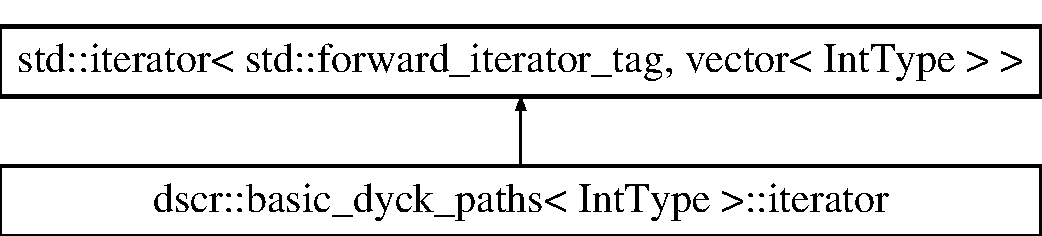
\includegraphics[height=2.000000cm]{classdscr_1_1basic__dyck__paths_1_1iterator}
\end{center}
\end{figure}
\subsection*{Public Member Functions}
\begin{DoxyCompactItemize}
\item 
\hypertarget{classdscr_1_1basic__dyck__paths_1_1iterator_a0323d0185a3384bf76f48b0efda2c768}{{\bfseries iterator} (Int\-Type n)}\label{classdscr_1_1basic__dyck__paths_1_1iterator_a0323d0185a3384bf76f48b0efda2c768}

\item 
\hypertarget{classdscr_1_1basic__dyck__paths_1_1iterator_a535c9355718debded4d16b4e117f3518}{\hyperlink{classdscr_1_1basic__dyck__paths_1_1iterator}{iterator} \& {\bfseries operator++} ()}\label{classdscr_1_1basic__dyck__paths_1_1iterator_a535c9355718debded4d16b4e117f3518}

\item 
\hypertarget{classdscr_1_1basic__dyck__paths_1_1iterator_aa51059634f27303e1811eea66139c967}{\hyperlink{classdscr_1_1basic__dyck__paths_1_1iterator}{iterator} \& {\bfseries operator-\/-\/} ()}\label{classdscr_1_1basic__dyck__paths_1_1iterator_aa51059634f27303e1811eea66139c967}

\item 
\hypertarget{classdscr_1_1basic__dyck__paths_1_1iterator_a59d03d522f4f0c11e6ac9db883a16050}{const vector$<$ Int\-Type $>$ \& {\bfseries operator$\ast$} () const }\label{classdscr_1_1basic__dyck__paths_1_1iterator_a59d03d522f4f0c11e6ac9db883a16050}

\item 
\hypertarget{classdscr_1_1basic__dyck__paths_1_1iterator_a1c762819f673390c4b80d4766cef929e}{const dyck\-\_\-path $\ast$ {\bfseries operator-\/$>$} () const }\label{classdscr_1_1basic__dyck__paths_1_1iterator_a1c762819f673390c4b80d4766cef929e}

\item 
\hypertarget{classdscr_1_1basic__dyck__paths_1_1iterator_a2cb194fd591f4639f26ded5e15a57eb4}{size\-\_\-type {\bfseries I\-D} () const }\label{classdscr_1_1basic__dyck__paths_1_1iterator_a2cb194fd591f4639f26ded5e15a57eb4}

\item 
\hypertarget{classdscr_1_1basic__dyck__paths_1_1iterator_ac733d2dbea4d7324c13a638f457f0fd6}{bool {\bfseries operator==} (const \hyperlink{classdscr_1_1basic__dyck__paths_1_1iterator}{iterator} \&it) const }\label{classdscr_1_1basic__dyck__paths_1_1iterator_ac733d2dbea4d7324c13a638f457f0fd6}

\item 
\hypertarget{classdscr_1_1basic__dyck__paths_1_1iterator_a7bc133fd5261e926c4dbfb489f09b3d8}{bool {\bfseries operator!=} (const \hyperlink{classdscr_1_1basic__dyck__paths_1_1iterator}{iterator} \&it) const }\label{classdscr_1_1basic__dyck__paths_1_1iterator_a7bc133fd5261e926c4dbfb489f09b3d8}

\item 
\hypertarget{classdscr_1_1basic__dyck__paths_1_1iterator_a3655a7c8464547eefd4bb0f3fc240bf3}{bool {\bfseries is\-\_\-at\-\_\-end} (Int\-Type n) const }\label{classdscr_1_1basic__dyck__paths_1_1iterator_a3655a7c8464547eefd4bb0f3fc240bf3}

\item 
\hypertarget{classdscr_1_1basic__dyck__paths_1_1iterator_a172fcff2c55aae9dc1073803b7554459}{void {\bfseries reset} (Int\-Type r)}\label{classdscr_1_1basic__dyck__paths_1_1iterator_a172fcff2c55aae9dc1073803b7554459}

\end{DoxyCompactItemize}
\subsection*{Friends}
\begin{DoxyCompactItemize}
\item 
\hypertarget{classdscr_1_1basic__dyck__paths_1_1iterator_a3dd4f1061ed68889e2068166aee9248a}{class {\bfseries basic\-\_\-dyck\-\_\-paths}}\label{classdscr_1_1basic__dyck__paths_1_1iterator_a3dd4f1061ed68889e2068166aee9248a}

\item 
\hypertarget{classdscr_1_1basic__dyck__paths_1_1iterator_a4304f5d7bb1d12de2d2ad2c1e4e64dab}{difference\-\_\-type {\bfseries operator-\/} (const \hyperlink{classdscr_1_1basic__dyck__paths_1_1iterator}{iterator} \&lhs, const \hyperlink{classdscr_1_1basic__dyck__paths_1_1iterator}{iterator} \&rhs)}\label{classdscr_1_1basic__dyck__paths_1_1iterator_a4304f5d7bb1d12de2d2ad2c1e4e64dab}

\end{DoxyCompactItemize}


\subsection{Detailed Description}
\subsubsection*{template$<$class Int\-Type$>$class dscr\-::basic\-\_\-dyck\-\_\-paths$<$ Int\-Type $>$\-::iterator}

Forward iterator class. 

The documentation for this class was generated from the following file\-:\begin{DoxyCompactItemize}
\item 
Dyck\-Paths.\-hpp\end{DoxyCompactItemize}

\hypertarget{classdscr_1_1basic__motzkin__paths_1_1iterator}{\section{dscr\-:\-:basic\-\_\-motzkin\-\_\-paths$<$ Int\-Type $>$\-:\-:iterator Class Reference}
\label{classdscr_1_1basic__motzkin__paths_1_1iterator}\index{dscr\-::basic\-\_\-motzkin\-\_\-paths$<$ Int\-Type $>$\-::iterator@{dscr\-::basic\-\_\-motzkin\-\_\-paths$<$ Int\-Type $>$\-::iterator}}
}


Forward iterator class.  




{\ttfamily \#include $<$Motzkin.\-hpp$>$}

Inheritance diagram for dscr\-:\-:basic\-\_\-motzkin\-\_\-paths$<$ Int\-Type $>$\-:\-:iterator\-:\begin{figure}[H]
\begin{center}
\leavevmode
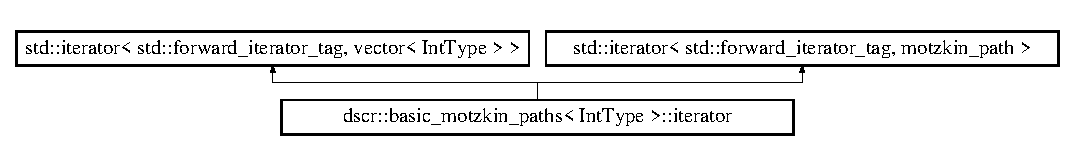
\includegraphics[height=1.586402cm]{classdscr_1_1basic__motzkin__paths_1_1iterator}
\end{center}
\end{figure}
\subsection*{Public Member Functions}
\begin{DoxyCompactItemize}
\item 
\hypertarget{classdscr_1_1basic__motzkin__paths_1_1iterator_a49c7980f9fcd34f6fccec84f58f5c6ee}{{\bfseries iterator} (Int\-Type n)}\label{classdscr_1_1basic__motzkin__paths_1_1iterator_a49c7980f9fcd34f6fccec84f58f5c6ee}

\item 
\hypertarget{classdscr_1_1basic__motzkin__paths_1_1iterator_af32864d4dbb0868c64e267d99507b3f7}{\hyperlink{classdscr_1_1basic__motzkin__paths_1_1iterator}{iterator} \& {\bfseries operator++} ()}\label{classdscr_1_1basic__motzkin__paths_1_1iterator_af32864d4dbb0868c64e267d99507b3f7}

\item 
\hypertarget{classdscr_1_1basic__motzkin__paths_1_1iterator_ae32aed14099167c8d26f5faf2472066e}{\hyperlink{classdscr_1_1basic__motzkin__paths_1_1iterator}{iterator} \& {\bfseries operator-\/-\/} ()}\label{classdscr_1_1basic__motzkin__paths_1_1iterator_ae32aed14099167c8d26f5faf2472066e}

\item 
\hypertarget{classdscr_1_1basic__motzkin__paths_1_1iterator_aad98d526351ba6e8f28502a7aeaeecbe}{const vector$<$ Int\-Type $>$ \& {\bfseries operator$\ast$} () const }\label{classdscr_1_1basic__motzkin__paths_1_1iterator_aad98d526351ba6e8f28502a7aeaeecbe}

\item 
\hypertarget{classdscr_1_1basic__motzkin__paths_1_1iterator_a3773a4876e2b879c4c03fac75d0030ed}{const motzkin\-\_\-path $\ast$ {\bfseries operator-\/$>$} () const }\label{classdscr_1_1basic__motzkin__paths_1_1iterator_a3773a4876e2b879c4c03fac75d0030ed}

\item 
\hypertarget{classdscr_1_1basic__motzkin__paths_1_1iterator_acb1f7ca6a55be9f538fb0a437d82396a}{size\-\_\-type {\bfseries I\-D} () const }\label{classdscr_1_1basic__motzkin__paths_1_1iterator_acb1f7ca6a55be9f538fb0a437d82396a}

\item 
\hypertarget{classdscr_1_1basic__motzkin__paths_1_1iterator_a85fa122e0dd60a04f6093c2b4c967359}{bool {\bfseries operator==} (const \hyperlink{classdscr_1_1basic__motzkin__paths_1_1iterator}{iterator} \&it) const }\label{classdscr_1_1basic__motzkin__paths_1_1iterator_a85fa122e0dd60a04f6093c2b4c967359}

\item 
\hypertarget{classdscr_1_1basic__motzkin__paths_1_1iterator_ac85ddedcb5d359644719845b7cdf50b2}{bool {\bfseries operator!=} (const \hyperlink{classdscr_1_1basic__motzkin__paths_1_1iterator}{iterator} \&it) const }\label{classdscr_1_1basic__motzkin__paths_1_1iterator_ac85ddedcb5d359644719845b7cdf50b2}

\item 
\hypertarget{classdscr_1_1basic__motzkin__paths_1_1iterator_a2ab5b9ee66e7f2c35f0677302e4c1eec}{void {\bfseries reset} (Int\-Type n)}\label{classdscr_1_1basic__motzkin__paths_1_1iterator_a2ab5b9ee66e7f2c35f0677302e4c1eec}

\item 
\hypertarget{classdscr_1_1basic__motzkin__paths_1_1iterator_af5da85fe0786b8d763e4d7e28ac2a05a}{{\bfseries iterator} (int n)}\label{classdscr_1_1basic__motzkin__paths_1_1iterator_af5da85fe0786b8d763e4d7e28ac2a05a}

\item 
\hypertarget{classdscr_1_1basic__motzkin__paths_1_1iterator_af32864d4dbb0868c64e267d99507b3f7}{\hyperlink{classdscr_1_1basic__motzkin__paths_1_1iterator}{iterator} \& {\bfseries operator++} ()}\label{classdscr_1_1basic__motzkin__paths_1_1iterator_af32864d4dbb0868c64e267d99507b3f7}

\item 
\hypertarget{classdscr_1_1basic__motzkin__paths_1_1iterator_aad98d526351ba6e8f28502a7aeaeecbe}{const vector$<$ Int\-Type $>$ \& {\bfseries operator$\ast$} () const }\label{classdscr_1_1basic__motzkin__paths_1_1iterator_aad98d526351ba6e8f28502a7aeaeecbe}

\item 
\hypertarget{classdscr_1_1basic__motzkin__paths_1_1iterator_acce870919b833403e42b92611ae7746d}{vector$<$ Int\-Type $>$ \& {\bfseries operator$\ast$} ()}\label{classdscr_1_1basic__motzkin__paths_1_1iterator_acce870919b833403e42b92611ae7746d}

\item 
\hypertarget{classdscr_1_1basic__motzkin__paths_1_1iterator_a85fa122e0dd60a04f6093c2b4c967359}{bool {\bfseries operator==} (const \hyperlink{classdscr_1_1basic__motzkin__paths_1_1iterator}{iterator} \&it) const }\label{classdscr_1_1basic__motzkin__paths_1_1iterator_a85fa122e0dd60a04f6093c2b4c967359}

\item 
\hypertarget{classdscr_1_1basic__motzkin__paths_1_1iterator_ac85ddedcb5d359644719845b7cdf50b2}{bool {\bfseries operator!=} (const \hyperlink{classdscr_1_1basic__motzkin__paths_1_1iterator}{iterator} \&it) const }\label{classdscr_1_1basic__motzkin__paths_1_1iterator_ac85ddedcb5d359644719845b7cdf50b2}

\end{DoxyCompactItemize}
\subsection*{Friends}
\begin{DoxyCompactItemize}
\item 
\hypertarget{classdscr_1_1basic__motzkin__paths_1_1iterator_a63be6a774fd8c390bcfc98a78e52930d}{class {\bfseries basic\-\_\-motzkin\-\_\-paths}}\label{classdscr_1_1basic__motzkin__paths_1_1iterator_a63be6a774fd8c390bcfc98a78e52930d}

\item 
\hypertarget{classdscr_1_1basic__motzkin__paths_1_1iterator_a4304f5d7bb1d12de2d2ad2c1e4e64dab}{difference\-\_\-type {\bfseries operator-\/} (const \hyperlink{classdscr_1_1basic__motzkin__paths_1_1iterator}{iterator} \&lhs, const \hyperlink{classdscr_1_1basic__motzkin__paths_1_1iterator}{iterator} \&rhs)}\label{classdscr_1_1basic__motzkin__paths_1_1iterator_a4304f5d7bb1d12de2d2ad2c1e4e64dab}

\end{DoxyCompactItemize}


\subsection{Detailed Description}
\subsubsection*{template$<$class Int\-Type$>$class dscr\-::basic\-\_\-motzkin\-\_\-paths$<$ Int\-Type $>$\-::iterator}

Forward iterator class. 

The documentation for this class was generated from the following files\-:\begin{DoxyCompactItemize}
\item 
Motzkin.\-hpp\item 
motzkinold.\-hpp\end{DoxyCompactItemize}

\hypertarget{classdscr_1_1basic__multisets_1_1iterator}{\section{dscr\-:\-:basic\-\_\-multisets$<$ Int\-Type $>$\-:\-:iterator Class Reference}
\label{classdscr_1_1basic__multisets_1_1iterator}\index{dscr\-::basic\-\_\-multisets$<$ Int\-Type $>$\-::iterator@{dscr\-::basic\-\_\-multisets$<$ Int\-Type $>$\-::iterator}}
}
Inheritance diagram for dscr\-:\-:basic\-\_\-multisets$<$ Int\-Type $>$\-:\-:iterator\-:\begin{figure}[H]
\begin{center}
\leavevmode
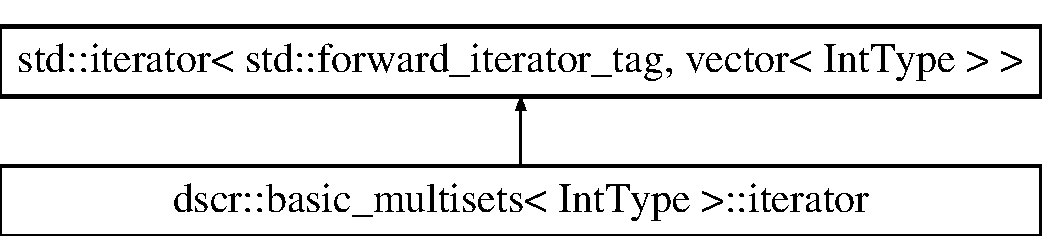
\includegraphics[height=2.000000cm]{classdscr_1_1basic__multisets_1_1iterator}
\end{center}
\end{figure}
\subsection*{Public Member Functions}
\begin{DoxyCompactItemize}
\item 
\hypertarget{classdscr_1_1basic__multisets_1_1iterator_a8593f477dc6ea42b78dc7a09ca8780af}{{\bfseries iterator} (const vector$<$ Int\-Type $>$ \&total)}\label{classdscr_1_1basic__multisets_1_1iterator_a8593f477dc6ea42b78dc7a09ca8780af}

\item 
\hypertarget{classdscr_1_1basic__multisets_1_1iterator_ab8efc236871cafe7ecabc93f62efaee4}{\hyperlink{classdscr_1_1basic__multisets_1_1iterator}{iterator} \& {\bfseries operator++} ()}\label{classdscr_1_1basic__multisets_1_1iterator_ab8efc236871cafe7ecabc93f62efaee4}

\item 
\hypertarget{classdscr_1_1basic__multisets_1_1iterator_a0951c43ba6d231de238c47a421889879}{const vector$<$ Int\-Type $>$ \& {\bfseries operator$\ast$} () const }\label{classdscr_1_1basic__multisets_1_1iterator_a0951c43ba6d231de238c47a421889879}

\item 
\hypertarget{classdscr_1_1basic__multisets_1_1iterator_a25922f0c1bfee770223acda648277174}{vector$<$ Int\-Type $>$ \& {\bfseries operator$\ast$} ()}\label{classdscr_1_1basic__multisets_1_1iterator_a25922f0c1bfee770223acda648277174}

\item 
\hypertarget{classdscr_1_1basic__multisets_1_1iterator_a4198bdfea6b080c891581363097f0513}{bool {\bfseries operator==} (const \hyperlink{classdscr_1_1basic__multisets_1_1iterator}{iterator} \&it) const }\label{classdscr_1_1basic__multisets_1_1iterator_a4198bdfea6b080c891581363097f0513}

\item 
\hypertarget{classdscr_1_1basic__multisets_1_1iterator_a66da6fbeba7a333b4160472bb3f90046}{bool {\bfseries operator!=} (const \hyperlink{classdscr_1_1basic__multisets_1_1iterator}{iterator} \&it) const }\label{classdscr_1_1basic__multisets_1_1iterator_a66da6fbeba7a333b4160472bb3f90046}

\end{DoxyCompactItemize}
\subsection*{Friends}
\begin{DoxyCompactItemize}
\item 
\hypertarget{classdscr_1_1basic__multisets_1_1iterator_a92dc798fe1da23a96a2138fadd200c4a}{class {\bfseries basic\-\_\-multisets}}\label{classdscr_1_1basic__multisets_1_1iterator_a92dc798fe1da23a96a2138fadd200c4a}

\end{DoxyCompactItemize}


The documentation for this class was generated from the following file\-:\begin{DoxyCompactItemize}
\item 
Multisets.\-hpp\end{DoxyCompactItemize}

\hypertarget{classdscr_1_1basic__partitions_1_1iterator}{\section{dscr\-:\-:basic\-\_\-partitions$<$ Int\-Type $>$\-:\-:iterator Class Reference}
\label{classdscr_1_1basic__partitions_1_1iterator}\index{dscr\-::basic\-\_\-partitions$<$ Int\-Type $>$\-::iterator@{dscr\-::basic\-\_\-partitions$<$ Int\-Type $>$\-::iterator}}
}


Forward iterator class.  




{\ttfamily \#include $<$Partitions.\-hpp$>$}

Inheritance diagram for dscr\-:\-:basic\-\_\-partitions$<$ Int\-Type $>$\-:\-:iterator\-:\begin{figure}[H]
\begin{center}
\leavevmode
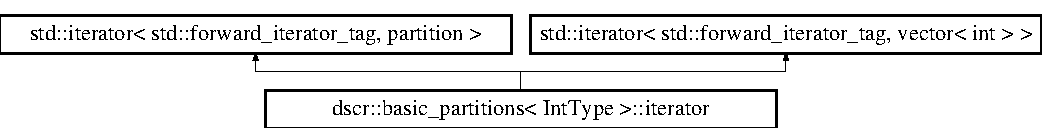
\includegraphics[height=2.000000cm]{classdscr_1_1basic__partitions_1_1iterator}
\end{center}
\end{figure}
\subsection*{Public Member Functions}
\begin{DoxyCompactItemize}
\item 
\hypertarget{classdscr_1_1basic__partitions_1_1iterator_a889b266d3dcfc9c88e389d4a7b642c2c}{{\bfseries iterator} (Int\-Type n, Int\-Type numparts)}\label{classdscr_1_1basic__partitions_1_1iterator_a889b266d3dcfc9c88e389d4a7b642c2c}

\item 
\hypertarget{classdscr_1_1basic__partitions_1_1iterator_a4c8308f225ce78db2592767705cefdf2}{\hyperlink{classdscr_1_1basic__partitions_1_1iterator}{iterator} \& {\bfseries operator++} ()}\label{classdscr_1_1basic__partitions_1_1iterator_a4c8308f225ce78db2592767705cefdf2}

\item 
\hypertarget{classdscr_1_1basic__partitions_1_1iterator_a8f184daf98f836bd070b4b08f0284c31}{const vector$<$ Int\-Type $>$ \& {\bfseries operator$\ast$} () const }\label{classdscr_1_1basic__partitions_1_1iterator_a8f184daf98f836bd070b4b08f0284c31}

\item 
\hypertarget{classdscr_1_1basic__partitions_1_1iterator_a738d7b084322462a69e272ba9aec70bc}{const partition $\ast$ {\bfseries operator-\/$>$} () const }\label{classdscr_1_1basic__partitions_1_1iterator_a738d7b084322462a69e272ba9aec70bc}

\item 
\hypertarget{classdscr_1_1basic__partitions_1_1iterator_a7b629e122ab601f1d8445e3cbca0111a}{size\-\_\-type {\bfseries I\-D} () const }\label{classdscr_1_1basic__partitions_1_1iterator_a7b629e122ab601f1d8445e3cbca0111a}

\item 
\hypertarget{classdscr_1_1basic__partitions_1_1iterator_af7bbea4b59964923bacfa12b226f19d4}{bool {\bfseries operator==} (const \hyperlink{classdscr_1_1basic__partitions_1_1iterator}{iterator} \&it) const }\label{classdscr_1_1basic__partitions_1_1iterator_af7bbea4b59964923bacfa12b226f19d4}

\item 
\hypertarget{classdscr_1_1basic__partitions_1_1iterator_a5b89d704e3d35a15749fe492cfeb2e52}{bool {\bfseries operator!=} (const \hyperlink{classdscr_1_1basic__partitions_1_1iterator}{iterator} \&it) const }\label{classdscr_1_1basic__partitions_1_1iterator_a5b89d704e3d35a15749fe492cfeb2e52}

\end{DoxyCompactItemize}
\subsection*{Friends}
\begin{DoxyCompactItemize}
\item 
\hypertarget{classdscr_1_1basic__partitions_1_1iterator_aa61a5712b0e94d9ea6b10b06e861e942}{class {\bfseries basic\-\_\-partitions}}\label{classdscr_1_1basic__partitions_1_1iterator_aa61a5712b0e94d9ea6b10b06e861e942}

\item 
\hypertarget{classdscr_1_1basic__partitions_1_1iterator_a4304f5d7bb1d12de2d2ad2c1e4e64dab}{difference\-\_\-type {\bfseries operator-\/} (const \hyperlink{classdscr_1_1basic__partitions_1_1iterator}{iterator} \&lhs, const \hyperlink{classdscr_1_1basic__partitions_1_1iterator}{iterator} \&rhs)}\label{classdscr_1_1basic__partitions_1_1iterator_a4304f5d7bb1d12de2d2ad2c1e4e64dab}

\end{DoxyCompactItemize}


\subsection{Detailed Description}
\subsubsection*{template$<$class Int\-Type$>$class dscr\-::basic\-\_\-partitions$<$ Int\-Type $>$\-::iterator}

Forward iterator class. 

The documentation for this class was generated from the following file\-:\begin{DoxyCompactItemize}
\item 
Partitions.\-hpp\end{DoxyCompactItemize}

\hypertarget{classdscr_1_1basic__combinations_1_1iterator}{\section{dscr\-:\-:basic\-\_\-combinations$<$ Int\-Type $>$\-:\-:iterator Class Reference}
\label{classdscr_1_1basic__combinations_1_1iterator}\index{dscr\-::basic\-\_\-combinations$<$ Int\-Type $>$\-::iterator@{dscr\-::basic\-\_\-combinations$<$ Int\-Type $>$\-::iterator}}
}


Random access iterator class. It's much more efficient as a bidirectional iterator than purely random access.  




{\ttfamily \#include $<$Combinations.\-hpp$>$}

Inheritance diagram for dscr\-:\-:basic\-\_\-combinations$<$ Int\-Type $>$\-:\-:iterator\-:\begin{figure}[H]
\begin{center}
\leavevmode
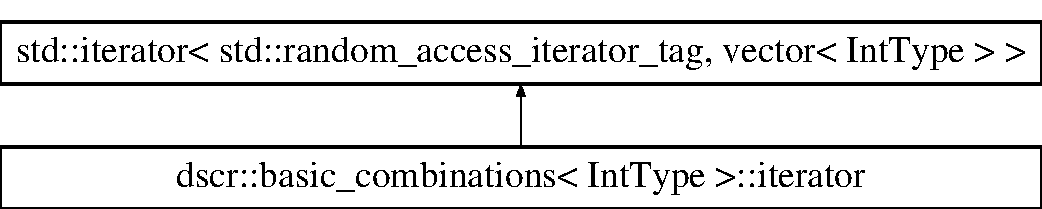
\includegraphics[height=2.000000cm]{classdscr_1_1basic__combinations_1_1iterator}
\end{center}
\end{figure}
\subsection*{Public Member Functions}
\begin{DoxyCompactItemize}
\item 
\hypertarget{classdscr_1_1basic__combinations_1_1iterator_a2f1cd9b3e8e6a14ab421e169ab3e3d26}{{\bfseries iterator} (Int\-Type n, Int\-Type r)}\label{classdscr_1_1basic__combinations_1_1iterator_a2f1cd9b3e8e6a14ab421e169ab3e3d26}

\item 
\hypertarget{classdscr_1_1basic__combinations_1_1iterator_aa0a91bda1b42222e2a1b693ec7ddf256}{\hyperlink{classdscr_1_1basic__combinations_1_1iterator}{iterator} \& {\bfseries operator++} ()}\label{classdscr_1_1basic__combinations_1_1iterator_aa0a91bda1b42222e2a1b693ec7ddf256}

\item 
\hypertarget{classdscr_1_1basic__combinations_1_1iterator_a559c5d01b13686afa8269fe33c7f9c31}{\hyperlink{classdscr_1_1basic__combinations_1_1iterator}{iterator} \& {\bfseries operator-\/-\/} ()}\label{classdscr_1_1basic__combinations_1_1iterator_a559c5d01b13686afa8269fe33c7f9c31}

\item 
\hypertarget{classdscr_1_1basic__combinations_1_1iterator_a822970dec9022e44d6b978b778e6dacc}{const vector$<$ Int\-Type $>$ \& {\bfseries operator$\ast$} () const }\label{classdscr_1_1basic__combinations_1_1iterator_a822970dec9022e44d6b978b778e6dacc}

\item 
\hypertarget{classdscr_1_1basic__combinations_1_1iterator_ade4f65e7376272f9eb05a0987729d51c}{const combination $\ast$ {\bfseries operator-\/$>$} () const }\label{classdscr_1_1basic__combinations_1_1iterator_ade4f65e7376272f9eb05a0987729d51c}

\item 
\hyperlink{classdscr_1_1basic__combinations_1_1iterator}{iterator} \& \hyperlink{classdscr_1_1basic__combinations_1_1iterator_aefdf7d30409efa626a178f1fc9495d8c}{operator+=} (difference\-\_\-type n)
\begin{DoxyCompactList}\small\item\em Random access capabilities to the iterators. \end{DoxyCompactList}\item 
\hypertarget{classdscr_1_1basic__combinations_1_1iterator_a151132962c20e63c5c9ad37ba6520d2d}{\hyperlink{classdscr_1_1basic__combinations_1_1iterator}{iterator} \& {\bfseries operator-\/=} (difference\-\_\-type n)}\label{classdscr_1_1basic__combinations_1_1iterator_a151132962c20e63c5c9ad37ba6520d2d}

\item 
\hypertarget{classdscr_1_1basic__combinations_1_1iterator_a1ef5fc403b15b1d5b337d430dde9ae38}{size\-\_\-type {\bfseries I\-D} () const }\label{classdscr_1_1basic__combinations_1_1iterator_a1ef5fc403b15b1d5b337d430dde9ae38}

\item 
\hypertarget{classdscr_1_1basic__combinations_1_1iterator_a905e6dbc06b760d379f5c7b70843609e}{bool {\bfseries operator==} (const \hyperlink{classdscr_1_1basic__combinations_1_1iterator}{iterator} \&it) const }\label{classdscr_1_1basic__combinations_1_1iterator_a905e6dbc06b760d379f5c7b70843609e}

\item 
\hypertarget{classdscr_1_1basic__combinations_1_1iterator_a05875ea91e2fdeb08f0caafd478695fa}{bool {\bfseries operator!=} (const \hyperlink{classdscr_1_1basic__combinations_1_1iterator}{iterator} \&it) const }\label{classdscr_1_1basic__combinations_1_1iterator_a05875ea91e2fdeb08f0caafd478695fa}

\item 
\hypertarget{classdscr_1_1basic__combinations_1_1iterator_a56057c892382d0299ea49a37768768d0}{bool {\bfseries is\-\_\-at\-\_\-end} (Int\-Type n) const }\label{classdscr_1_1basic__combinations_1_1iterator_a56057c892382d0299ea49a37768768d0}

\item 
\hypertarget{classdscr_1_1basic__combinations_1_1iterator_ab29b79c7e726f29d92d19383474edc3e}{void {\bfseries reset} (Int\-Type n, Int\-Type r)}\label{classdscr_1_1basic__combinations_1_1iterator_ab29b79c7e726f29d92d19383474edc3e}

\end{DoxyCompactItemize}
\subsection*{Friends}
\begin{DoxyCompactItemize}
\item 
\hypertarget{classdscr_1_1basic__combinations_1_1iterator_a5aee9caa75ebeddad7d54e7f4931ce21}{class {\bfseries basic\-\_\-combinations}}\label{classdscr_1_1basic__combinations_1_1iterator_a5aee9caa75ebeddad7d54e7f4931ce21}

\item 
\hypertarget{classdscr_1_1basic__combinations_1_1iterator_aac5493422e75e70b321e439c45168fd0}{\hyperlink{classdscr_1_1basic__combinations_1_1iterator}{iterator} {\bfseries operator+} (\hyperlink{classdscr_1_1basic__combinations_1_1iterator}{iterator} lhs, difference\-\_\-type n)}\label{classdscr_1_1basic__combinations_1_1iterator_aac5493422e75e70b321e439c45168fd0}

\item 
\hypertarget{classdscr_1_1basic__combinations_1_1iterator_a87727d9351117b3726fbeac5da5eb28c}{\hyperlink{classdscr_1_1basic__combinations_1_1iterator}{iterator} {\bfseries operator-\/} (\hyperlink{classdscr_1_1basic__combinations_1_1iterator}{iterator} lhs, difference\-\_\-type n)}\label{classdscr_1_1basic__combinations_1_1iterator_a87727d9351117b3726fbeac5da5eb28c}

\item 
\hypertarget{classdscr_1_1basic__combinations_1_1iterator_a4304f5d7bb1d12de2d2ad2c1e4e64dab}{difference\-\_\-type {\bfseries operator-\/} (const \hyperlink{classdscr_1_1basic__combinations_1_1iterator}{iterator} \&lhs, const \hyperlink{classdscr_1_1basic__combinations_1_1iterator}{iterator} \&rhs)}\label{classdscr_1_1basic__combinations_1_1iterator_a4304f5d7bb1d12de2d2ad2c1e4e64dab}

\end{DoxyCompactItemize}


\subsection{Detailed Description}
\subsubsection*{template$<$class Int\-Type$>$class dscr\-::basic\-\_\-combinations$<$ Int\-Type $>$\-::iterator}

Random access iterator class. It's much more efficient as a bidirectional iterator than purely random access. 

\subsection{Member Function Documentation}
\hypertarget{classdscr_1_1basic__combinations_1_1iterator_aefdf7d30409efa626a178f1fc9495d8c}{\index{dscr\-::basic\-\_\-combinations\-::iterator@{dscr\-::basic\-\_\-combinations\-::iterator}!operator+=@{operator+=}}
\index{operator+=@{operator+=}!dscr::basic_combinations::iterator@{dscr\-::basic\-\_\-combinations\-::iterator}}
\subsubsection[{operator+=}]{\setlength{\rightskip}{0pt plus 5cm}template$<$class Int\-Type $>$ {\bf iterator}\& {\bf dscr\-::basic\-\_\-combinations}$<$ Int\-Type $>$\-::iterator\-::operator+= (
\begin{DoxyParamCaption}
\item[{difference\-\_\-type}]{n}
\end{DoxyParamCaption}
)\hspace{0.3cm}{\ttfamily [inline]}}}\label{classdscr_1_1basic__combinations_1_1iterator_aefdf7d30409efa626a178f1fc9495d8c}


Random access capabilities to the iterators. 


\begin{DoxyParams}{Parameters}
{\em n} & -\/$>$ This assumes 0 $<$= n+\-I\-D $<$= size(n,k) \\
\hline
\end{DoxyParams}


The documentation for this class was generated from the following file\-:\begin{DoxyCompactItemize}
\item 
Combinations.\-hpp\end{DoxyCompactItemize}

\hypertarget{classdscr_1_1range_1_1iterator}{\section{dscr\-:\-:range$<$ Int\-Type $>$\-:\-:iterator Class Reference}
\label{classdscr_1_1range_1_1iterator}\index{dscr\-::range$<$ Int\-Type $>$\-::iterator@{dscr\-::range$<$ Int\-Type $>$\-::iterator}}
}


Random access iterator class.  




{\ttfamily \#include $<$Range.\-hpp$>$}

Inheritance diagram for dscr\-:\-:range$<$ Int\-Type $>$\-:\-:iterator\-:\begin{figure}[H]
\begin{center}
\leavevmode
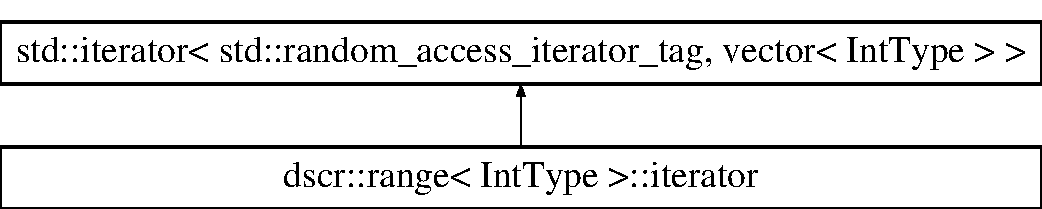
\includegraphics[height=2.000000cm]{classdscr_1_1range_1_1iterator}
\end{center}
\end{figure}
\subsection*{Public Member Functions}
\begin{DoxyCompactItemize}
\item 
\hypertarget{classdscr_1_1range_1_1iterator_ad5739009b166911bcb779206a4d5bbbb}{{\bfseries iterator} (size\-\_\-type t\-\_\-from)}\label{classdscr_1_1range_1_1iterator_ad5739009b166911bcb779206a4d5bbbb}

\item 
\hypertarget{classdscr_1_1range_1_1iterator_aa906c38a3b44ef70646a07f947da361d}{{\bfseries iterator} (size\-\_\-type t\-\_\-from, size\-\_\-type t\-\_\-step)}\label{classdscr_1_1range_1_1iterator_aa906c38a3b44ef70646a07f947da361d}

\item 
\hypertarget{classdscr_1_1range_1_1iterator_aa0cca1019fe8ceb036372e18964c2049}{\hyperlink{classdscr_1_1range_1_1iterator}{iterator} \& {\bfseries operator++} ()}\label{classdscr_1_1range_1_1iterator_aa0cca1019fe8ceb036372e18964c2049}

\item 
\hypertarget{classdscr_1_1range_1_1iterator_a1aba58c2b46819f4461bdf1e37dc295d}{\hyperlink{classdscr_1_1range_1_1iterator}{iterator} \& {\bfseries operator-\/-\/} ()}\label{classdscr_1_1range_1_1iterator_a1aba58c2b46819f4461bdf1e37dc295d}

\item 
\hypertarget{classdscr_1_1range_1_1iterator_a3a3522b36fd251dec273c9929893eaae}{const Int\-Type \& {\bfseries operator$\ast$} () const }\label{classdscr_1_1range_1_1iterator_a3a3522b36fd251dec273c9929893eaae}

\item 
\hyperlink{classdscr_1_1range_1_1iterator}{iterator} \& \hyperlink{classdscr_1_1range_1_1iterator_a33c9bfae559f304396651e146bef86dd}{operator+=} (long int n)
\begin{DoxyCompactList}\small\item\em Random access capabilities to the iterators. \end{DoxyCompactList}\item 
\hypertarget{classdscr_1_1range_1_1iterator_aac567b57428445fbdd91e0a18ca76509}{\hyperlink{classdscr_1_1range_1_1iterator}{iterator} \& {\bfseries operator-\/=} (long int n)}\label{classdscr_1_1range_1_1iterator_aac567b57428445fbdd91e0a18ca76509}

\item 
\hypertarget{classdscr_1_1range_1_1iterator_a95c26706e52ca57f186accc005fe1dbb}{bool {\bfseries operator==} (const \hyperlink{classdscr_1_1range_1_1iterator}{iterator} \&it)}\label{classdscr_1_1range_1_1iterator_a95c26706e52ca57f186accc005fe1dbb}

\item 
\hypertarget{classdscr_1_1range_1_1iterator_a7f079722eb4030388de622774657ff5e}{bool {\bfseries operator!=} (const \hyperlink{classdscr_1_1range_1_1iterator}{iterator} \&it)}\label{classdscr_1_1range_1_1iterator_a7f079722eb4030388de622774657ff5e}

\item 
\hypertarget{classdscr_1_1range_1_1iterator_a6282c8597291ec16f501ea910fe9a116}{difference\-\_\-type {\bfseries operator-\/} (const \hyperlink{classdscr_1_1range_1_1iterator}{iterator} \&it)}\label{classdscr_1_1range_1_1iterator_a6282c8597291ec16f501ea910fe9a116}

\item 
\hypertarget{classdscr_1_1range_1_1iterator_acb164839b228c61dc47261bc99c71395}{size\-\_\-type {\bfseries step} () const }\label{classdscr_1_1range_1_1iterator_acb164839b228c61dc47261bc99c71395}

\end{DoxyCompactItemize}
\subsection*{Friends}
\begin{DoxyCompactItemize}
\item 
\hypertarget{classdscr_1_1range_1_1iterator_a982e754214d3a01b73c8a27323b791c0}{class {\bfseries range}}\label{classdscr_1_1range_1_1iterator_a982e754214d3a01b73c8a27323b791c0}

\end{DoxyCompactItemize}


\subsection{Detailed Description}
\subsubsection*{template$<$class Int\-Type$>$class dscr\-::range$<$ Int\-Type $>$\-::iterator}

Random access iterator class. 

\subsection{Member Function Documentation}
\hypertarget{classdscr_1_1range_1_1iterator_a33c9bfae559f304396651e146bef86dd}{\index{dscr\-::range\-::iterator@{dscr\-::range\-::iterator}!operator+=@{operator+=}}
\index{operator+=@{operator+=}!dscr::range::iterator@{dscr\-::range\-::iterator}}
\subsubsection[{operator+=}]{\setlength{\rightskip}{0pt plus 5cm}template$<$class Int\-Type $>$ {\bf iterator}\& {\bf dscr\-::range}$<$ Int\-Type $>$\-::iterator\-::operator+= (
\begin{DoxyParamCaption}
\item[{long int}]{n}
\end{DoxyParamCaption}
)\hspace{0.3cm}{\ttfamily [inline]}}}\label{classdscr_1_1range_1_1iterator_a33c9bfae559f304396651e146bef86dd}


Random access capabilities to the iterators. 


\begin{DoxyParams}{Parameters}
{\em n} & -\/$>$ This assumes 0 $<$= n+\-I\-D $<$= size(n) \\
\hline
\end{DoxyParams}


The documentation for this class was generated from the following file\-:\begin{DoxyCompactItemize}
\item 
Range.\-hpp\end{DoxyCompactItemize}

\hypertarget{classdscr_1_1basic__subsets_1_1iterator}{\section{dscr\-:\-:basic\-\_\-subsets$<$ Bool\-Type $>$\-:\-:iterator Class Reference}
\label{classdscr_1_1basic__subsets_1_1iterator}\index{dscr\-::basic\-\_\-subsets$<$ Bool\-Type $>$\-::iterator@{dscr\-::basic\-\_\-subsets$<$ Bool\-Type $>$\-::iterator}}
}


Random access iterator class. It's much more efficient as a bidirectional iterator than purely random access.  




{\ttfamily \#include $<$Subsets.\-hpp$>$}

Inheritance diagram for dscr\-:\-:basic\-\_\-subsets$<$ Bool\-Type $>$\-:\-:iterator\-:\begin{figure}[H]
\begin{center}
\leavevmode
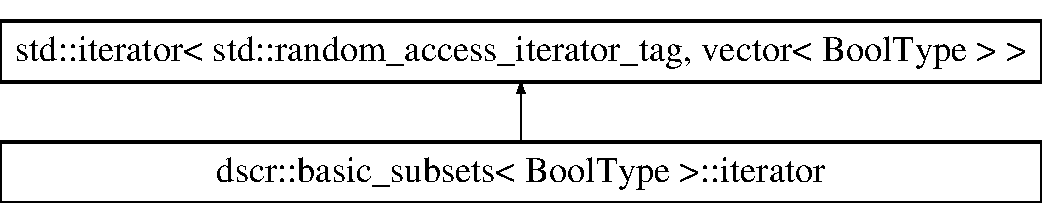
\includegraphics[height=2.000000cm]{classdscr_1_1basic__subsets_1_1iterator}
\end{center}
\end{figure}
\subsection*{Public Member Functions}
\begin{DoxyCompactItemize}
\item 
\hypertarget{classdscr_1_1basic__subsets_1_1iterator_a1ef45fec843ae0c298080ef1827a1e9d}{{\bfseries iterator} (size\-\_\-t n)}\label{classdscr_1_1basic__subsets_1_1iterator_a1ef45fec843ae0c298080ef1827a1e9d}

\item 
\hypertarget{classdscr_1_1basic__subsets_1_1iterator_ae7acb9cf5aad999dceba4e56aba024ca}{\hyperlink{classdscr_1_1basic__subsets_1_1iterator}{iterator} \& {\bfseries operator++} ()}\label{classdscr_1_1basic__subsets_1_1iterator_ae7acb9cf5aad999dceba4e56aba024ca}

\item 
\hypertarget{classdscr_1_1basic__subsets_1_1iterator_a5d0bd6baa7fba5ea9d141f658da0eb0f}{\hyperlink{classdscr_1_1basic__subsets_1_1iterator}{iterator} \& {\bfseries operator-\/-\/} ()}\label{classdscr_1_1basic__subsets_1_1iterator_a5d0bd6baa7fba5ea9d141f658da0eb0f}

\item 
\hypertarget{classdscr_1_1basic__subsets_1_1iterator_a90673aefa67ab5ef3bba771208d0642b}{const vector$<$ Bool\-Type $>$ \& {\bfseries operator$\ast$} () const }\label{classdscr_1_1basic__subsets_1_1iterator_a90673aefa67ab5ef3bba771208d0642b}

\item 
\hyperlink{classdscr_1_1basic__subsets_1_1iterator}{iterator} \& \hyperlink{classdscr_1_1basic__subsets_1_1iterator_ac67f07763f7f4e95dbeb056af75ccc6d}{operator+=} (difference\-\_\-type n)
\begin{DoxyCompactList}\small\item\em Random access capabilities to the iterators. \end{DoxyCompactList}\item 
\hypertarget{classdscr_1_1basic__subsets_1_1iterator_a23e311a6c5505bf8a61635e79d1a173d}{\hyperlink{classdscr_1_1basic__subsets_1_1iterator}{iterator} \& {\bfseries operator-\/=} (difference\-\_\-type n)}\label{classdscr_1_1basic__subsets_1_1iterator_a23e311a6c5505bf8a61635e79d1a173d}

\item 
\hypertarget{classdscr_1_1basic__subsets_1_1iterator_ae6ae9eb08d7574dda97f63f330f6dc95}{size\-\_\-type {\bfseries I\-D} () const }\label{classdscr_1_1basic__subsets_1_1iterator_ae6ae9eb08d7574dda97f63f330f6dc95}

\item 
\hypertarget{classdscr_1_1basic__subsets_1_1iterator_acf794053af10b30233d8d7f1401e952a}{bool {\bfseries operator==} (const \hyperlink{classdscr_1_1basic__subsets_1_1iterator}{iterator} \&it) const }\label{classdscr_1_1basic__subsets_1_1iterator_acf794053af10b30233d8d7f1401e952a}

\item 
\hypertarget{classdscr_1_1basic__subsets_1_1iterator_ae1210e20c8624d9a0b6f09a850be26d8}{bool {\bfseries operator!=} (const \hyperlink{classdscr_1_1basic__subsets_1_1iterator}{iterator} \&it) const }\label{classdscr_1_1basic__subsets_1_1iterator_ae1210e20c8624d9a0b6f09a850be26d8}

\item 
\hypertarget{classdscr_1_1basic__subsets_1_1iterator_ad5cac03a81c8ffa5768c32df4258448e}{bool {\bfseries is\-\_\-at\-\_\-end} (size\-\_\-t n) const }\label{classdscr_1_1basic__subsets_1_1iterator_ad5cac03a81c8ffa5768c32df4258448e}

\item 
\hypertarget{classdscr_1_1basic__subsets_1_1iterator_a210f08dcc1436aa7d37e407386d1992a}{void {\bfseries reset} (size\-\_\-t n)}\label{classdscr_1_1basic__subsets_1_1iterator_a210f08dcc1436aa7d37e407386d1992a}

\end{DoxyCompactItemize}
\subsection*{Friends}
\begin{DoxyCompactItemize}
\item 
\hypertarget{classdscr_1_1basic__subsets_1_1iterator_a6cf8333f0bc6a559385b55c16b45e772}{class {\bfseries basic\-\_\-subsets}}\label{classdscr_1_1basic__subsets_1_1iterator_a6cf8333f0bc6a559385b55c16b45e772}

\item 
\hypertarget{classdscr_1_1basic__subsets_1_1iterator_aac5493422e75e70b321e439c45168fd0}{\hyperlink{classdscr_1_1basic__subsets_1_1iterator}{iterator} {\bfseries operator+} (\hyperlink{classdscr_1_1basic__subsets_1_1iterator}{iterator} lhs, difference\-\_\-type n)}\label{classdscr_1_1basic__subsets_1_1iterator_aac5493422e75e70b321e439c45168fd0}

\item 
\hypertarget{classdscr_1_1basic__subsets_1_1iterator_a87727d9351117b3726fbeac5da5eb28c}{\hyperlink{classdscr_1_1basic__subsets_1_1iterator}{iterator} {\bfseries operator-\/} (\hyperlink{classdscr_1_1basic__subsets_1_1iterator}{iterator} lhs, difference\-\_\-type n)}\label{classdscr_1_1basic__subsets_1_1iterator_a87727d9351117b3726fbeac5da5eb28c}

\item 
\hypertarget{classdscr_1_1basic__subsets_1_1iterator_a4304f5d7bb1d12de2d2ad2c1e4e64dab}{difference\-\_\-type {\bfseries operator-\/} (const \hyperlink{classdscr_1_1basic__subsets_1_1iterator}{iterator} \&lhs, const \hyperlink{classdscr_1_1basic__subsets_1_1iterator}{iterator} \&rhs)}\label{classdscr_1_1basic__subsets_1_1iterator_a4304f5d7bb1d12de2d2ad2c1e4e64dab}

\end{DoxyCompactItemize}


\subsection{Detailed Description}
\subsubsection*{template$<$class Bool\-Type$>$class dscr\-::basic\-\_\-subsets$<$ Bool\-Type $>$\-::iterator}

Random access iterator class. It's much more efficient as a bidirectional iterator than purely random access. 

\subsection{Member Function Documentation}
\hypertarget{classdscr_1_1basic__subsets_1_1iterator_ac67f07763f7f4e95dbeb056af75ccc6d}{\index{dscr\-::basic\-\_\-subsets\-::iterator@{dscr\-::basic\-\_\-subsets\-::iterator}!operator+=@{operator+=}}
\index{operator+=@{operator+=}!dscr::basic_subsets::iterator@{dscr\-::basic\-\_\-subsets\-::iterator}}
\subsubsection[{operator+=}]{\setlength{\rightskip}{0pt plus 5cm}template$<$class Bool\-Type $>$ {\bf iterator}\& {\bf dscr\-::basic\-\_\-subsets}$<$ Bool\-Type $>$\-::iterator\-::operator+= (
\begin{DoxyParamCaption}
\item[{difference\-\_\-type}]{n}
\end{DoxyParamCaption}
)\hspace{0.3cm}{\ttfamily [inline]}}}\label{classdscr_1_1basic__subsets_1_1iterator_ac67f07763f7f4e95dbeb056af75ccc6d}


Random access capabilities to the iterators. 


\begin{DoxyParams}{Parameters}
{\em n} & -\/$>$ This assumes 0 $<$= n+\-I\-D $<$= size(n,k) \\
\hline
\end{DoxyParams}


The documentation for this class was generated from the following file\-:\begin{DoxyCompactItemize}
\item 
Subsets.\-hpp\end{DoxyCompactItemize}

\hypertarget{classdscr_1_1basic__permutations_1_1iterator}{\section{dscr\-:\-:basic\-\_\-permutations$<$ Int\-Type $>$\-:\-:iterator Class Reference}
\label{classdscr_1_1basic__permutations_1_1iterator}\index{dscr\-::basic\-\_\-permutations$<$ Int\-Type $>$\-::iterator@{dscr\-::basic\-\_\-permutations$<$ Int\-Type $>$\-::iterator}}
}


Random access iterator class. It's much more efficient as a bidirectional iterator than purely random access.  




{\ttfamily \#include $<$Permutations.\-hpp$>$}

Inheritance diagram for dscr\-:\-:basic\-\_\-permutations$<$ Int\-Type $>$\-:\-:iterator\-:\begin{figure}[H]
\begin{center}
\leavevmode
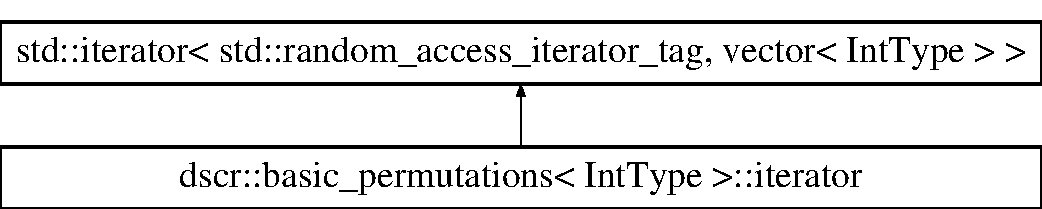
\includegraphics[height=2.000000cm]{classdscr_1_1basic__permutations_1_1iterator}
\end{center}
\end{figure}
\subsection*{Public Member Functions}
\begin{DoxyCompactItemize}
\item 
\hypertarget{classdscr_1_1basic__permutations_1_1iterator_a42aba4a30c7d9225c0108afdd0471982}{{\bfseries iterator} (Int\-Type n)}\label{classdscr_1_1basic__permutations_1_1iterator_a42aba4a30c7d9225c0108afdd0471982}

\item 
\hypertarget{classdscr_1_1basic__permutations_1_1iterator_a2db24401b75963582838437bafeed1d8}{\hyperlink{classdscr_1_1basic__permutations_1_1iterator}{iterator} \& {\bfseries operator++} ()}\label{classdscr_1_1basic__permutations_1_1iterator_a2db24401b75963582838437bafeed1d8}

\item 
\hypertarget{classdscr_1_1basic__permutations_1_1iterator_acb908cc12a7babf06669fc1452394e09}{\hyperlink{classdscr_1_1basic__permutations_1_1iterator}{iterator} \& {\bfseries operator-\/-\/} ()}\label{classdscr_1_1basic__permutations_1_1iterator_acb908cc12a7babf06669fc1452394e09}

\item 
\hypertarget{classdscr_1_1basic__permutations_1_1iterator_a1e12a3351b0ae1be085b23fb0bebdc44}{const vector$<$ Int\-Type $>$ \& {\bfseries operator$\ast$} () const }\label{classdscr_1_1basic__permutations_1_1iterator_a1e12a3351b0ae1be085b23fb0bebdc44}

\item 
\hyperlink{classdscr_1_1basic__permutations_1_1iterator}{iterator} \& \hyperlink{classdscr_1_1basic__permutations_1_1iterator_a89238333e4ca83dd4d75f62c709f9ff1}{operator+=} (long int n)
\begin{DoxyCompactList}\small\item\em Random access capabilities to the iterators. \end{DoxyCompactList}\item 
\hypertarget{classdscr_1_1basic__permutations_1_1iterator_a4a57770c7df7ac3441d59d552d01e874}{\hyperlink{classdscr_1_1basic__permutations_1_1iterator}{iterator} \& {\bfseries operator-\/=} (long int n)}\label{classdscr_1_1basic__permutations_1_1iterator_a4a57770c7df7ac3441d59d552d01e874}

\item 
\hypertarget{classdscr_1_1basic__permutations_1_1iterator_a0fbeac6dafcec1feb5c0d5f4f697c87c}{size\-\_\-type {\bfseries I\-D} () const }\label{classdscr_1_1basic__permutations_1_1iterator_a0fbeac6dafcec1feb5c0d5f4f697c87c}

\item 
\hypertarget{classdscr_1_1basic__permutations_1_1iterator_a02a668ac35c4370a5ab04b40be271a51}{bool {\bfseries operator==} (const \hyperlink{classdscr_1_1basic__permutations_1_1iterator}{iterator} \&it) const }\label{classdscr_1_1basic__permutations_1_1iterator_a02a668ac35c4370a5ab04b40be271a51}

\item 
\hypertarget{classdscr_1_1basic__permutations_1_1iterator_a664c38decc9fee5565e6020f45f1aed3}{bool {\bfseries operator!=} (const \hyperlink{classdscr_1_1basic__permutations_1_1iterator}{iterator} \&it) const }\label{classdscr_1_1basic__permutations_1_1iterator_a664c38decc9fee5565e6020f45f1aed3}

\item 
\hypertarget{classdscr_1_1basic__permutations_1_1iterator_affc892ba834515195f3c90d7e1b08438}{bool {\bfseries is\-\_\-at\-\_\-end} (Int\-Type n) const }\label{classdscr_1_1basic__permutations_1_1iterator_affc892ba834515195f3c90d7e1b08438}

\item 
\hypertarget{classdscr_1_1basic__permutations_1_1iterator_ab64642914f8ad33ae3dff63386d2283c}{void {\bfseries reset} (Int\-Type r)}\label{classdscr_1_1basic__permutations_1_1iterator_ab64642914f8ad33ae3dff63386d2283c}

\end{DoxyCompactItemize}
\subsection*{Friends}
\begin{DoxyCompactItemize}
\item 
\hypertarget{classdscr_1_1basic__permutations_1_1iterator_a99f81faf0718d566d11f4d1a4ad187ba}{class {\bfseries basic\-\_\-permutations}}\label{classdscr_1_1basic__permutations_1_1iterator_a99f81faf0718d566d11f4d1a4ad187ba}

\item 
\hypertarget{classdscr_1_1basic__permutations_1_1iterator_aac5493422e75e70b321e439c45168fd0}{\hyperlink{classdscr_1_1basic__permutations_1_1iterator}{iterator} {\bfseries operator+} (\hyperlink{classdscr_1_1basic__permutations_1_1iterator}{iterator} lhs, difference\-\_\-type n)}\label{classdscr_1_1basic__permutations_1_1iterator_aac5493422e75e70b321e439c45168fd0}

\item 
\hypertarget{classdscr_1_1basic__permutations_1_1iterator_a87727d9351117b3726fbeac5da5eb28c}{\hyperlink{classdscr_1_1basic__permutations_1_1iterator}{iterator} {\bfseries operator-\/} (\hyperlink{classdscr_1_1basic__permutations_1_1iterator}{iterator} lhs, difference\-\_\-type n)}\label{classdscr_1_1basic__permutations_1_1iterator_a87727d9351117b3726fbeac5da5eb28c}

\item 
\hypertarget{classdscr_1_1basic__permutations_1_1iterator_a4304f5d7bb1d12de2d2ad2c1e4e64dab}{difference\-\_\-type {\bfseries operator-\/} (const \hyperlink{classdscr_1_1basic__permutations_1_1iterator}{iterator} \&lhs, const \hyperlink{classdscr_1_1basic__permutations_1_1iterator}{iterator} \&rhs)}\label{classdscr_1_1basic__permutations_1_1iterator_a4304f5d7bb1d12de2d2ad2c1e4e64dab}

\end{DoxyCompactItemize}


\subsection{Detailed Description}
\subsubsection*{template$<$class Int\-Type$>$class dscr\-::basic\-\_\-permutations$<$ Int\-Type $>$\-::iterator}

Random access iterator class. It's much more efficient as a bidirectional iterator than purely random access. 

\subsection{Member Function Documentation}
\hypertarget{classdscr_1_1basic__permutations_1_1iterator_a89238333e4ca83dd4d75f62c709f9ff1}{\index{dscr\-::basic\-\_\-permutations\-::iterator@{dscr\-::basic\-\_\-permutations\-::iterator}!operator+=@{operator+=}}
\index{operator+=@{operator+=}!dscr::basic_permutations::iterator@{dscr\-::basic\-\_\-permutations\-::iterator}}
\subsubsection[{operator+=}]{\setlength{\rightskip}{0pt plus 5cm}template$<$class Int\-Type $>$ {\bf iterator}\& {\bf dscr\-::basic\-\_\-permutations}$<$ Int\-Type $>$\-::iterator\-::operator+= (
\begin{DoxyParamCaption}
\item[{long int}]{n}
\end{DoxyParamCaption}
)\hspace{0.3cm}{\ttfamily [inline]}}}\label{classdscr_1_1basic__permutations_1_1iterator_a89238333e4ca83dd4d75f62c709f9ff1}


Random access capabilities to the iterators. 


\begin{DoxyParams}{Parameters}
{\em n} & -\/$>$ This assumes 0 $<$= n+\-I\-D $<$= size(n,k) \\
\hline
\end{DoxyParams}


The documentation for this class was generated from the following file\-:\begin{DoxyCompactItemize}
\item 
Permutations.\-hpp\end{DoxyCompactItemize}

\hypertarget{classdscr_1_1range}{\section{dscr\-:\-:range$<$ Int\-Type $>$ Class Template Reference}
\label{classdscr_1_1range}\index{dscr\-::range$<$ Int\-Type $>$@{dscr\-::range$<$ Int\-Type $>$}}
}


Similar to python range(n) or range(n,m) or range(n,m,step).  




{\ttfamily \#include $<$Range.\-hpp$>$}

\subsection*{Classes}
\begin{DoxyCompactItemize}
\item 
class \hyperlink{classdscr_1_1range_1_1iterator}{iterator}
\begin{DoxyCompactList}\small\item\em Random access iterator class. \end{DoxyCompactList}\end{DoxyCompactItemize}
\subsection*{Public Types}
\begin{DoxyCompactItemize}
\item 
\hypertarget{classdscr_1_1range_a9103a7d7e47ee61a4573fc90b807d68f}{typedef long int {\bfseries difference\-\_\-type}}\label{classdscr_1_1range_a9103a7d7e47ee61a4573fc90b807d68f}

\item 
\hypertarget{classdscr_1_1range_acc40f3c534fdf9efcbeea0de92d650ba}{typedef Int\-Type {\bfseries size\-\_\-type}}\label{classdscr_1_1range_acc40f3c534fdf9efcbeea0de92d650ba}

\item 
\hypertarget{classdscr_1_1range_ab64808d7c694e90230fd27b90f8256ab}{typedef Int\-Type {\bfseries value\-\_\-type}}\label{classdscr_1_1range_ab64808d7c694e90230fd27b90f8256ab}

\end{DoxyCompactItemize}
\subsection*{Public Member Functions}
\begin{DoxyCompactItemize}
\item 
\hyperlink{classdscr_1_1range_a06f0f16f812d432d88dd8588f29f3181}{range} (Int\-Type n)
\begin{DoxyCompactList}\small\item\em Constructor. \end{DoxyCompactList}\item 
\hypertarget{classdscr_1_1range_a4ad29f26b18f04b589bff44b72cf4d3d}{{\bfseries range} (Int\-Type t\-\_\-from, Int\-Type t\-\_\-to, Int\-Type t\-\_\-step=1)}\label{classdscr_1_1range_a4ad29f26b18f04b589bff44b72cf4d3d}

\item 
\hypertarget{classdscr_1_1range_a5c6479d75d8a1e2309cf64eaa8502a3f}{size\-\_\-type {\bfseries size} () const }\label{classdscr_1_1range_a5c6479d75d8a1e2309cf64eaa8502a3f}

\item 
\hypertarget{classdscr_1_1range_a7089c881081d554ffd65408b43750875}{{\bfseries operator vector$<$ Int\-Type $>$} () const }\label{classdscr_1_1range_a7089c881081d554ffd65408b43750875}

\item 
\hypertarget{classdscr_1_1range_ab779841b574efbfe5ff839126d0d581d}{const \hyperlink{classdscr_1_1range_1_1iterator}{iterator} \& {\bfseries begin} () const }\label{classdscr_1_1range_ab779841b574efbfe5ff839126d0d581d}

\item 
\hypertarget{classdscr_1_1range_a63c2677015e157b5fbfb98d47cf28073}{const \hyperlink{classdscr_1_1range_1_1iterator}{iterator} \& {\bfseries end} () const }\label{classdscr_1_1range_a63c2677015e157b5fbfb98d47cf28073}

\item 
\hypertarget{classdscr_1_1range_af959a5570e78ea9aa1f9ffc088e8347d}{Int\-Type {\bfseries operator\mbox{[}$\,$\mbox{]}} (size\-\_\-type m) const }\label{classdscr_1_1range_af959a5570e78ea9aa1f9ffc088e8347d}

\end{DoxyCompactItemize}


\subsection{Detailed Description}
\subsubsection*{template$<$class Int\-Type$>$class dscr\-::range$<$ Int\-Type $>$}

Similar to python range(n) or range(n,m) or range(n,m,step). 


\begin{DoxyParams}{Parameters}
{\em n} & is an integer \\
\hline
\end{DoxyParams}
\begin{DoxyReturn}{Returns}
an abstract random-\/access container whose elements are \{n,n+1,n+2,...,m-\/1\} 
\end{DoxyReturn}


\subsection{Constructor \& Destructor Documentation}
\hypertarget{classdscr_1_1range_a06f0f16f812d432d88dd8588f29f3181}{\index{dscr\-::range@{dscr\-::range}!range@{range}}
\index{range@{range}!dscr::range@{dscr\-::range}}
\subsubsection[{range}]{\setlength{\rightskip}{0pt plus 5cm}template$<$class Int\-Type $>$ {\bf dscr\-::range}$<$ Int\-Type $>$\-::{\bf range} (
\begin{DoxyParamCaption}
\item[{Int\-Type}]{n}
\end{DoxyParamCaption}
)\hspace{0.3cm}{\ttfamily [inline]}}}\label{classdscr_1_1range_a06f0f16f812d432d88dd8588f29f3181}


Constructor. 


\begin{DoxyParams}{Parameters}
{\em n} & is an integer $>$= 0 \\
\hline
\end{DoxyParams}


The documentation for this class was generated from the following file\-:\begin{DoxyCompactItemize}
\item 
Range.\-hpp\end{DoxyCompactItemize}

\hypertarget{classdscr_1_1_r_clock}{\section{dscr\-:\-:R\-Clock Class Reference}
\label{classdscr_1_1_r_clock}\index{dscr\-::\-R\-Clock@{dscr\-::\-R\-Clock}}
}
\subsection*{Static Public Member Functions}
\begin{DoxyCompactItemize}
\item 
\hypertarget{classdscr_1_1_r_clock_a10bfd78f1ec37b2d1fc1d79fac81ea1b}{static \hyperlink{classdscr_1_1_r_clock}{R\-Clock} \& {\bfseries Instance} ()}\label{classdscr_1_1_r_clock_a10bfd78f1ec37b2d1fc1d79fac81ea1b}

\end{DoxyCompactItemize}
\subsection*{Public Attributes}
\begin{DoxyCompactItemize}
\item 
\hypertarget{classdscr_1_1_r_clock_aedf7313152181172e967d8a927f5e92e}{std\-::chrono\-::time\-\_\-point\\*
$<$ std\-::chrono\-::high\-\_\-resolution\-\_\-clock $>$ {\bfseries start\-\_\-timer}}\label{classdscr_1_1_r_clock_aedf7313152181172e967d8a927f5e92e}

\item 
\hypertarget{classdscr_1_1_r_clock_aa0ef70fb9ab23841cbc12058f9325454}{std\-::chrono\-::time\-\_\-point\\*
$<$ std\-::chrono\-::high\-\_\-resolution\-\_\-clock $>$ {\bfseries running\-\_\-timer}}\label{classdscr_1_1_r_clock_aa0ef70fb9ab23841cbc12058f9325454}

\end{DoxyCompactItemize}


The documentation for this class was generated from the following file\-:\begin{DoxyCompactItemize}
\item 
Time\-Helpers.\-hpp\end{DoxyCompactItemize}

\hypertarget{classdscr_1_1basic__subsets_1_1reverse__iterator}{\section{dscr\-:\-:basic\-\_\-subsets$<$ Bool\-Type $>$\-:\-:reverse\-\_\-iterator Class Reference}
\label{classdscr_1_1basic__subsets_1_1reverse__iterator}\index{dscr\-::basic\-\_\-subsets$<$ Bool\-Type $>$\-::reverse\-\_\-iterator@{dscr\-::basic\-\_\-subsets$<$ Bool\-Type $>$\-::reverse\-\_\-iterator}}
}


Reverse random access iterator class. It's much more efficient as a bidirectional iterator than purely random access.  




{\ttfamily \#include $<$Subsets.\-hpp$>$}

Inheritance diagram for dscr\-:\-:basic\-\_\-subsets$<$ Bool\-Type $>$\-:\-:reverse\-\_\-iterator\-:\begin{figure}[H]
\begin{center}
\leavevmode
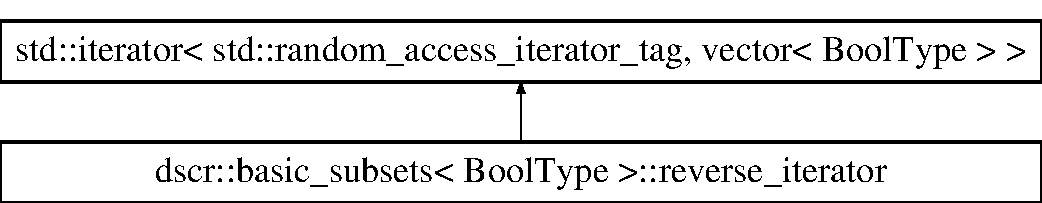
\includegraphics[height=2.000000cm]{classdscr_1_1basic__subsets_1_1reverse__iterator}
\end{center}
\end{figure}
\subsection*{Public Member Functions}
\begin{DoxyCompactItemize}
\item 
\hypertarget{classdscr_1_1basic__subsets_1_1reverse__iterator_ae881491a0fde157aaf11032420afb1fa}{{\bfseries reverse\-\_\-iterator} (size\-\_\-t n)}\label{classdscr_1_1basic__subsets_1_1reverse__iterator_ae881491a0fde157aaf11032420afb1fa}

\item 
\hypertarget{classdscr_1_1basic__subsets_1_1reverse__iterator_a2e26596cd4eb08949f3f42125019c060}{\hyperlink{classdscr_1_1basic__subsets_1_1reverse__iterator}{reverse\-\_\-iterator} \& {\bfseries operator++} ()}\label{classdscr_1_1basic__subsets_1_1reverse__iterator_a2e26596cd4eb08949f3f42125019c060}

\item 
\hypertarget{classdscr_1_1basic__subsets_1_1reverse__iterator_ac2e6419244b3ed704db611d450b50851}{\hyperlink{classdscr_1_1basic__subsets_1_1reverse__iterator}{reverse\-\_\-iterator} \& {\bfseries operator-\/-\/} ()}\label{classdscr_1_1basic__subsets_1_1reverse__iterator_ac2e6419244b3ed704db611d450b50851}

\item 
\hypertarget{classdscr_1_1basic__subsets_1_1reverse__iterator_a2945789283c079d8d65ce0aa887fa26f}{const vector$<$ Bool\-Type $>$ \& {\bfseries operator$\ast$} ()}\label{classdscr_1_1basic__subsets_1_1reverse__iterator_a2945789283c079d8d65ce0aa887fa26f}

\item 
\hypertarget{classdscr_1_1basic__subsets_1_1reverse__iterator_af570bb42ca9407072796330f8e390be5}{const vector$<$ Bool\-Type $>$ \& {\bfseries operator$\ast$} () const }\label{classdscr_1_1basic__subsets_1_1reverse__iterator_af570bb42ca9407072796330f8e390be5}

\item 
\hyperlink{classdscr_1_1basic__subsets_1_1reverse__iterator}{reverse\-\_\-iterator} \& \hyperlink{classdscr_1_1basic__subsets_1_1reverse__iterator_ab2b67d473ba635a014dc88aa03fdbbd8}{operator+=} (difference\-\_\-type m)
\begin{DoxyCompactList}\small\item\em Random access capabilities to the iterators. \end{DoxyCompactList}\item 
\hypertarget{classdscr_1_1basic__subsets_1_1reverse__iterator_a4f9155dc056c0e6096ef875f19ea2a65}{\hyperlink{classdscr_1_1basic__subsets_1_1reverse__iterator}{reverse\-\_\-iterator} \& {\bfseries operator-\/=} (difference\-\_\-type n)}\label{classdscr_1_1basic__subsets_1_1reverse__iterator_a4f9155dc056c0e6096ef875f19ea2a65}

\item 
\hypertarget{classdscr_1_1basic__subsets_1_1reverse__iterator_a39450a95332955f0b9ae736327b17ce0}{size\-\_\-type {\bfseries I\-D} () const }\label{classdscr_1_1basic__subsets_1_1reverse__iterator_a39450a95332955f0b9ae736327b17ce0}

\item 
\hypertarget{classdscr_1_1basic__subsets_1_1reverse__iterator_af0953925852185e06dacdc2c02103700}{bool {\bfseries operator==} (const \hyperlink{classdscr_1_1basic__subsets_1_1reverse__iterator}{reverse\-\_\-iterator} \&it)}\label{classdscr_1_1basic__subsets_1_1reverse__iterator_af0953925852185e06dacdc2c02103700}

\item 
\hypertarget{classdscr_1_1basic__subsets_1_1reverse__iterator_a36b667527e25f2a49c904b6512f03d6d}{bool {\bfseries operator!=} (const \hyperlink{classdscr_1_1basic__subsets_1_1reverse__iterator}{reverse\-\_\-iterator} \&it)}\label{classdscr_1_1basic__subsets_1_1reverse__iterator_a36b667527e25f2a49c904b6512f03d6d}

\item 
\hypertarget{classdscr_1_1basic__subsets_1_1reverse__iterator_ae9f2c7579e8ae1b78e660c6ecbb244bf}{bool {\bfseries is\-\_\-at\-\_\-end} () const }\label{classdscr_1_1basic__subsets_1_1reverse__iterator_ae9f2c7579e8ae1b78e660c6ecbb244bf}

\item 
\hypertarget{classdscr_1_1basic__subsets_1_1reverse__iterator_a78076f4d2f12110485927b9525a10b57}{void {\bfseries reset} (Bool\-Type n)}\label{classdscr_1_1basic__subsets_1_1reverse__iterator_a78076f4d2f12110485927b9525a10b57}

\end{DoxyCompactItemize}
\subsection*{Friends}
\begin{DoxyCompactItemize}
\item 
\hypertarget{classdscr_1_1basic__subsets_1_1reverse__iterator_a6cf8333f0bc6a559385b55c16b45e772}{class {\bfseries basic\-\_\-subsets}}\label{classdscr_1_1basic__subsets_1_1reverse__iterator_a6cf8333f0bc6a559385b55c16b45e772}

\item 
\hypertarget{classdscr_1_1basic__subsets_1_1reverse__iterator_a2c7fdd81f663381e951fb677763da73a}{\hyperlink{classdscr_1_1basic__subsets_1_1reverse__iterator}{reverse\-\_\-iterator} {\bfseries operator+} (\hyperlink{classdscr_1_1basic__subsets_1_1reverse__iterator}{reverse\-\_\-iterator} lhs, difference\-\_\-type n)}\label{classdscr_1_1basic__subsets_1_1reverse__iterator_a2c7fdd81f663381e951fb677763da73a}

\item 
\hypertarget{classdscr_1_1basic__subsets_1_1reverse__iterator_ad23e7d190001b7e889291da869e0e825}{\hyperlink{classdscr_1_1basic__subsets_1_1reverse__iterator}{reverse\-\_\-iterator} {\bfseries operator-\/} (\hyperlink{classdscr_1_1basic__subsets_1_1reverse__iterator}{reverse\-\_\-iterator} lhs, difference\-\_\-type n)}\label{classdscr_1_1basic__subsets_1_1reverse__iterator_ad23e7d190001b7e889291da869e0e825}

\item 
\hypertarget{classdscr_1_1basic__subsets_1_1reverse__iterator_a46fe9efd66cb5e2a2e89a93f2e060b82}{difference\-\_\-type {\bfseries operator-\/} (const \hyperlink{classdscr_1_1basic__subsets_1_1reverse__iterator}{reverse\-\_\-iterator} \&lhs, const \hyperlink{classdscr_1_1basic__subsets_1_1reverse__iterator}{reverse\-\_\-iterator} \&rhs)}\label{classdscr_1_1basic__subsets_1_1reverse__iterator_a46fe9efd66cb5e2a2e89a93f2e060b82}

\end{DoxyCompactItemize}


\subsection{Detailed Description}
\subsubsection*{template$<$class Bool\-Type$>$class dscr\-::basic\-\_\-subsets$<$ Bool\-Type $>$\-::reverse\-\_\-iterator}

Reverse random access iterator class. It's much more efficient as a bidirectional iterator than purely random access. 

\subsection{Member Function Documentation}
\hypertarget{classdscr_1_1basic__subsets_1_1reverse__iterator_ab2b67d473ba635a014dc88aa03fdbbd8}{\index{dscr\-::basic\-\_\-subsets\-::reverse\-\_\-iterator@{dscr\-::basic\-\_\-subsets\-::reverse\-\_\-iterator}!operator+=@{operator+=}}
\index{operator+=@{operator+=}!dscr::basic_subsets::reverse_iterator@{dscr\-::basic\-\_\-subsets\-::reverse\-\_\-iterator}}
\subsubsection[{operator+=}]{\setlength{\rightskip}{0pt plus 5cm}template$<$class Bool\-Type $>$ {\bf reverse\-\_\-iterator}\& {\bf dscr\-::basic\-\_\-subsets}$<$ Bool\-Type $>$\-::reverse\-\_\-iterator\-::operator+= (
\begin{DoxyParamCaption}
\item[{difference\-\_\-type}]{m}
\end{DoxyParamCaption}
)\hspace{0.3cm}{\ttfamily [inline]}}}\label{classdscr_1_1basic__subsets_1_1reverse__iterator_ab2b67d473ba635a014dc88aa03fdbbd8}


Random access capabilities to the iterators. 


\begin{DoxyParams}{Parameters}
{\em n} & -\/$>$ This assumes 0 $<$= n+\-I\-D $<$= size(n,k) \\
\hline
\end{DoxyParams}


The documentation for this class was generated from the following file\-:\begin{DoxyCompactItemize}
\item 
Subsets.\-hpp\end{DoxyCompactItemize}

\hypertarget{classdscr_1_1basic__permutations_1_1reverse__iterator}{\section{dscr\-:\-:basic\-\_\-permutations$<$ Int\-Type $>$\-:\-:reverse\-\_\-iterator Class Reference}
\label{classdscr_1_1basic__permutations_1_1reverse__iterator}\index{dscr\-::basic\-\_\-permutations$<$ Int\-Type $>$\-::reverse\-\_\-iterator@{dscr\-::basic\-\_\-permutations$<$ Int\-Type $>$\-::reverse\-\_\-iterator}}
}


Reverse random access iterator class. It's much more efficient as a bidirectional iterator than purely random access.  




{\ttfamily \#include $<$Permutations.\-hpp$>$}

Inheritance diagram for dscr\-:\-:basic\-\_\-permutations$<$ Int\-Type $>$\-:\-:reverse\-\_\-iterator\-:\begin{figure}[H]
\begin{center}
\leavevmode
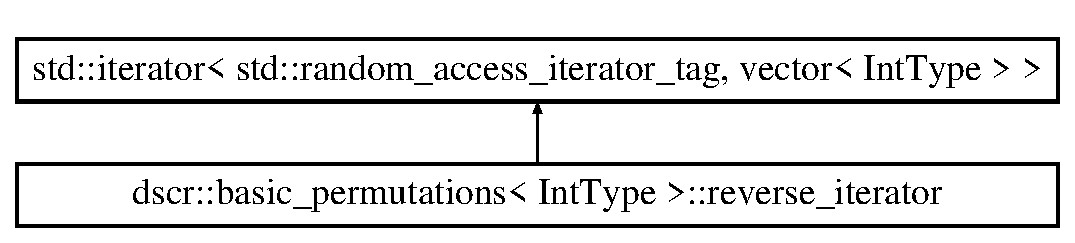
\includegraphics[height=2.000000cm]{classdscr_1_1basic__permutations_1_1reverse__iterator}
\end{center}
\end{figure}
\subsection*{Public Member Functions}
\begin{DoxyCompactItemize}
\item 
\hypertarget{classdscr_1_1basic__permutations_1_1reverse__iterator_a176b65db468d8d3e7b3f5926fa4c77b7}{{\bfseries reverse\-\_\-iterator} (Int\-Type n)}\label{classdscr_1_1basic__permutations_1_1reverse__iterator_a176b65db468d8d3e7b3f5926fa4c77b7}

\item 
\hypertarget{classdscr_1_1basic__permutations_1_1reverse__iterator_a799c7a1405b9b714df8e36a067379fd2}{\hyperlink{classdscr_1_1basic__permutations_1_1reverse__iterator}{reverse\-\_\-iterator} \& {\bfseries operator++} ()}\label{classdscr_1_1basic__permutations_1_1reverse__iterator_a799c7a1405b9b714df8e36a067379fd2}

\item 
\hypertarget{classdscr_1_1basic__permutations_1_1reverse__iterator_a75b82c902a21e2dffccaa17f8b7bcfbd}{\hyperlink{classdscr_1_1basic__permutations_1_1reverse__iterator}{reverse\-\_\-iterator} \& {\bfseries operator-\/-\/} ()}\label{classdscr_1_1basic__permutations_1_1reverse__iterator_a75b82c902a21e2dffccaa17f8b7bcfbd}

\item 
\hypertarget{classdscr_1_1basic__permutations_1_1reverse__iterator_a9894023c3115bbca64e1b1959c63eab7}{const permutation \& {\bfseries operator$\ast$} () const }\label{classdscr_1_1basic__permutations_1_1reverse__iterator_a9894023c3115bbca64e1b1959c63eab7}

\item 
\hyperlink{classdscr_1_1basic__permutations_1_1reverse__iterator}{reverse\-\_\-iterator} \& \hyperlink{classdscr_1_1basic__permutations_1_1reverse__iterator_a3306367f8c040072a0e5bc94077d5981}{operator+=} (long int m)
\begin{DoxyCompactList}\small\item\em Random access capabilities to the iterators. \end{DoxyCompactList}\item 
\hypertarget{classdscr_1_1basic__permutations_1_1reverse__iterator_ad036709f3a93cac6b351b813d841ebac}{\hyperlink{classdscr_1_1basic__permutations_1_1reverse__iterator}{reverse\-\_\-iterator} \& {\bfseries operator-\/=} (long int n)}\label{classdscr_1_1basic__permutations_1_1reverse__iterator_ad036709f3a93cac6b351b813d841ebac}

\item 
\hypertarget{classdscr_1_1basic__permutations_1_1reverse__iterator_a814e3f06d84287853961808f37ca3fe7}{size\-\_\-type {\bfseries I\-D} () const }\label{classdscr_1_1basic__permutations_1_1reverse__iterator_a814e3f06d84287853961808f37ca3fe7}

\item 
\hypertarget{classdscr_1_1basic__permutations_1_1reverse__iterator_a6b032acd3b59386b90238d105d040ea6}{bool {\bfseries operator==} (const \hyperlink{classdscr_1_1basic__permutations_1_1reverse__iterator}{reverse\-\_\-iterator} \&it) const }\label{classdscr_1_1basic__permutations_1_1reverse__iterator_a6b032acd3b59386b90238d105d040ea6}

\item 
\hypertarget{classdscr_1_1basic__permutations_1_1reverse__iterator_ac725b643ed1d3f021591f7ac46975785}{bool {\bfseries operator!=} (const \hyperlink{classdscr_1_1basic__permutations_1_1reverse__iterator}{reverse\-\_\-iterator} \&it) const }\label{classdscr_1_1basic__permutations_1_1reverse__iterator_ac725b643ed1d3f021591f7ac46975785}

\item 
\hypertarget{classdscr_1_1basic__permutations_1_1reverse__iterator_a4bdbc3a5b33186c1053e83790b142592}{void {\bfseries reset} (Int\-Type n)}\label{classdscr_1_1basic__permutations_1_1reverse__iterator_a4bdbc3a5b33186c1053e83790b142592}

\end{DoxyCompactItemize}
\subsection*{Friends}
\begin{DoxyCompactItemize}
\item 
\hypertarget{classdscr_1_1basic__permutations_1_1reverse__iterator_a99f81faf0718d566d11f4d1a4ad187ba}{class {\bfseries basic\-\_\-permutations}}\label{classdscr_1_1basic__permutations_1_1reverse__iterator_a99f81faf0718d566d11f4d1a4ad187ba}

\item 
\hypertarget{classdscr_1_1basic__permutations_1_1reverse__iterator_a2c7fdd81f663381e951fb677763da73a}{\hyperlink{classdscr_1_1basic__permutations_1_1reverse__iterator}{reverse\-\_\-iterator} {\bfseries operator+} (\hyperlink{classdscr_1_1basic__permutations_1_1reverse__iterator}{reverse\-\_\-iterator} lhs, difference\-\_\-type n)}\label{classdscr_1_1basic__permutations_1_1reverse__iterator_a2c7fdd81f663381e951fb677763da73a}

\item 
\hypertarget{classdscr_1_1basic__permutations_1_1reverse__iterator_ad23e7d190001b7e889291da869e0e825}{\hyperlink{classdscr_1_1basic__permutations_1_1reverse__iterator}{reverse\-\_\-iterator} {\bfseries operator-\/} (\hyperlink{classdscr_1_1basic__permutations_1_1reverse__iterator}{reverse\-\_\-iterator} lhs, difference\-\_\-type n)}\label{classdscr_1_1basic__permutations_1_1reverse__iterator_ad23e7d190001b7e889291da869e0e825}

\item 
\hypertarget{classdscr_1_1basic__permutations_1_1reverse__iterator_a46fe9efd66cb5e2a2e89a93f2e060b82}{difference\-\_\-type {\bfseries operator-\/} (const \hyperlink{classdscr_1_1basic__permutations_1_1reverse__iterator}{reverse\-\_\-iterator} \&lhs, const \hyperlink{classdscr_1_1basic__permutations_1_1reverse__iterator}{reverse\-\_\-iterator} \&rhs)}\label{classdscr_1_1basic__permutations_1_1reverse__iterator_a46fe9efd66cb5e2a2e89a93f2e060b82}

\end{DoxyCompactItemize}


\subsection{Detailed Description}
\subsubsection*{template$<$class Int\-Type$>$class dscr\-::basic\-\_\-permutations$<$ Int\-Type $>$\-::reverse\-\_\-iterator}

Reverse random access iterator class. It's much more efficient as a bidirectional iterator than purely random access. 

\subsection{Member Function Documentation}
\hypertarget{classdscr_1_1basic__permutations_1_1reverse__iterator_a3306367f8c040072a0e5bc94077d5981}{\index{dscr\-::basic\-\_\-permutations\-::reverse\-\_\-iterator@{dscr\-::basic\-\_\-permutations\-::reverse\-\_\-iterator}!operator+=@{operator+=}}
\index{operator+=@{operator+=}!dscr::basic_permutations::reverse_iterator@{dscr\-::basic\-\_\-permutations\-::reverse\-\_\-iterator}}
\subsubsection[{operator+=}]{\setlength{\rightskip}{0pt plus 5cm}template$<$class Int\-Type $>$ {\bf reverse\-\_\-iterator}\& {\bf dscr\-::basic\-\_\-permutations}$<$ Int\-Type $>$\-::reverse\-\_\-iterator\-::operator+= (
\begin{DoxyParamCaption}
\item[{long int}]{m}
\end{DoxyParamCaption}
)\hspace{0.3cm}{\ttfamily [inline]}}}\label{classdscr_1_1basic__permutations_1_1reverse__iterator_a3306367f8c040072a0e5bc94077d5981}


Random access capabilities to the iterators. 


\begin{DoxyParams}{Parameters}
{\em n} & -\/$>$ This assumes 0 $<$= n+\-I\-D $<$= size(n,k) \\
\hline
\end{DoxyParams}


The documentation for this class was generated from the following file\-:\begin{DoxyCompactItemize}
\item 
Permutations.\-hpp\end{DoxyCompactItemize}

\hypertarget{classdscr_1_1basic__partitions_1_1reverse__iterator}{\section{dscr\-:\-:basic\-\_\-partitions$<$ Int\-Type $>$\-:\-:reverse\-\_\-iterator Class Reference}
\label{classdscr_1_1basic__partitions_1_1reverse__iterator}\index{dscr\-::basic\-\_\-partitions$<$ Int\-Type $>$\-::reverse\-\_\-iterator@{dscr\-::basic\-\_\-partitions$<$ Int\-Type $>$\-::reverse\-\_\-iterator}}
}


Forward Iterator class.  




{\ttfamily \#include $<$Partitions.\-hpp$>$}

Inheritance diagram for dscr\-:\-:basic\-\_\-partitions$<$ Int\-Type $>$\-:\-:reverse\-\_\-iterator\-:\begin{figure}[H]
\begin{center}
\leavevmode
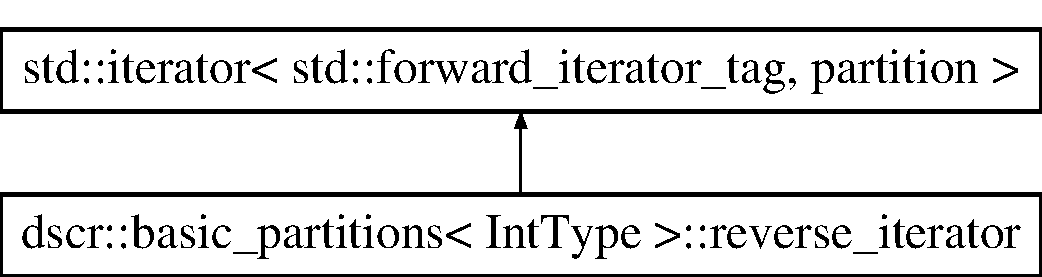
\includegraphics[height=2.000000cm]{classdscr_1_1basic__partitions_1_1reverse__iterator}
\end{center}
\end{figure}
\subsection*{Public Member Functions}
\begin{DoxyCompactItemize}
\item 
\hypertarget{classdscr_1_1basic__partitions_1_1reverse__iterator_ae2ebdfa3db2806231b3f75e52a5151f6}{{\bfseries reverse\-\_\-iterator} (Int\-Type n)}\label{classdscr_1_1basic__partitions_1_1reverse__iterator_ae2ebdfa3db2806231b3f75e52a5151f6}

\item 
\hypertarget{classdscr_1_1basic__partitions_1_1reverse__iterator_ad896606e31f1398b1231d5fe7c70a1fc}{\hyperlink{classdscr_1_1basic__partitions_1_1reverse__iterator}{reverse\-\_\-iterator} \& {\bfseries operator++} ()}\label{classdscr_1_1basic__partitions_1_1reverse__iterator_ad896606e31f1398b1231d5fe7c70a1fc}

\item 
\hypertarget{classdscr_1_1basic__partitions_1_1reverse__iterator_ad73f3a08be51f345a2e6207af8b85073}{\hyperlink{classdscr_1_1basic__partitions_1_1reverse__iterator}{reverse\-\_\-iterator} \& {\bfseries operator-\/-\/} ()}\label{classdscr_1_1basic__partitions_1_1reverse__iterator_ad73f3a08be51f345a2e6207af8b85073}

\item 
\hypertarget{classdscr_1_1basic__partitions_1_1reverse__iterator_a4526cd21a80f4b7c482db2161bc797c7}{const partition \& {\bfseries operator$\ast$} ()}\label{classdscr_1_1basic__partitions_1_1reverse__iterator_a4526cd21a80f4b7c482db2161bc797c7}

\item 
\hypertarget{classdscr_1_1basic__partitions_1_1reverse__iterator_a61375f25b428fd6f3809e9d28cca4520}{const partition \& {\bfseries operator$\ast$} () const }\label{classdscr_1_1basic__partitions_1_1reverse__iterator_a61375f25b428fd6f3809e9d28cca4520}

\item 
\hypertarget{classdscr_1_1basic__partitions_1_1reverse__iterator_a29b71207476be3bd855b060e8f6e1594}{const partition $\ast$ {\bfseries operator-\/$>$} () const }\label{classdscr_1_1basic__partitions_1_1reverse__iterator_a29b71207476be3bd855b060e8f6e1594}

\item 
\hypertarget{classdscr_1_1basic__partitions_1_1reverse__iterator_aeff2506fcdf25d703e1f9b2a481e7084}{size\-\_\-type {\bfseries I\-D} () const }\label{classdscr_1_1basic__partitions_1_1reverse__iterator_aeff2506fcdf25d703e1f9b2a481e7084}

\item 
\hypertarget{classdscr_1_1basic__partitions_1_1reverse__iterator_a9f6a5d577a5a626564e6c9398e19c155}{bool {\bfseries operator==} (const \hyperlink{classdscr_1_1basic__partitions_1_1reverse__iterator}{reverse\-\_\-iterator} \&it)}\label{classdscr_1_1basic__partitions_1_1reverse__iterator_a9f6a5d577a5a626564e6c9398e19c155}

\item 
\hypertarget{classdscr_1_1basic__partitions_1_1reverse__iterator_a0881f77607be7f6c75df751d47864ba1}{bool {\bfseries operator!=} (const \hyperlink{classdscr_1_1basic__partitions_1_1reverse__iterator}{reverse\-\_\-iterator} \&it)}\label{classdscr_1_1basic__partitions_1_1reverse__iterator_a0881f77607be7f6c75df751d47864ba1}

\end{DoxyCompactItemize}
\subsection*{Friends}
\begin{DoxyCompactItemize}
\item 
\hypertarget{classdscr_1_1basic__partitions_1_1reverse__iterator_aa61a5712b0e94d9ea6b10b06e861e942}{class {\bfseries basic\-\_\-partitions}}\label{classdscr_1_1basic__partitions_1_1reverse__iterator_aa61a5712b0e94d9ea6b10b06e861e942}

\item 
\hypertarget{classdscr_1_1basic__partitions_1_1reverse__iterator_a46fe9efd66cb5e2a2e89a93f2e060b82}{difference\-\_\-type {\bfseries operator-\/} (const \hyperlink{classdscr_1_1basic__partitions_1_1reverse__iterator}{reverse\-\_\-iterator} \&lhs, const \hyperlink{classdscr_1_1basic__partitions_1_1reverse__iterator}{reverse\-\_\-iterator} \&rhs)}\label{classdscr_1_1basic__partitions_1_1reverse__iterator_a46fe9efd66cb5e2a2e89a93f2e060b82}

\end{DoxyCompactItemize}


\subsection{Detailed Description}
\subsubsection*{template$<$class Int\-Type$>$class dscr\-::basic\-\_\-partitions$<$ Int\-Type $>$\-::reverse\-\_\-iterator}

Forward Iterator class. 

The documentation for this class was generated from the following file\-:\begin{DoxyCompactItemize}
\item 
Partitions.\-hpp\end{DoxyCompactItemize}

\hypertarget{classdscr_1_1basic__combinations_1_1reverse__iterator}{\section{dscr\-:\-:basic\-\_\-combinations$<$ Int\-Type $>$\-:\-:reverse\-\_\-iterator Class Reference}
\label{classdscr_1_1basic__combinations_1_1reverse__iterator}\index{dscr\-::basic\-\_\-combinations$<$ Int\-Type $>$\-::reverse\-\_\-iterator@{dscr\-::basic\-\_\-combinations$<$ Int\-Type $>$\-::reverse\-\_\-iterator}}
}


Reverse random access iterator class. It's much more efficient as a bidirectional iterator than purely random access.  




{\ttfamily \#include $<$Combinations.\-hpp$>$}

Inheritance diagram for dscr\-:\-:basic\-\_\-combinations$<$ Int\-Type $>$\-:\-:reverse\-\_\-iterator\-:\begin{figure}[H]
\begin{center}
\leavevmode
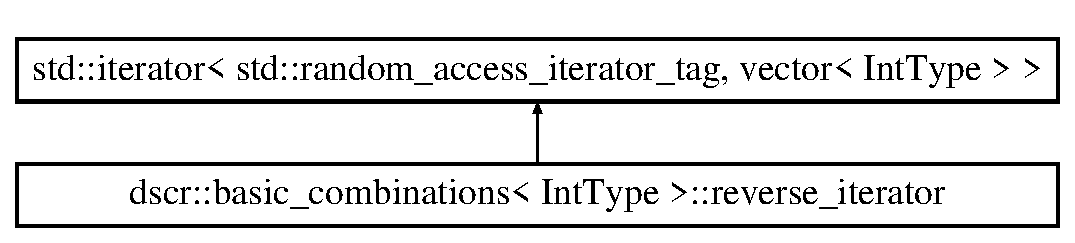
\includegraphics[height=2.000000cm]{classdscr_1_1basic__combinations_1_1reverse__iterator}
\end{center}
\end{figure}
\subsection*{Public Member Functions}
\begin{DoxyCompactItemize}
\item 
\hypertarget{classdscr_1_1basic__combinations_1_1reverse__iterator_a24545715b1327620ec976eb049afe826}{{\bfseries reverse\-\_\-iterator} (Int\-Type n, Int\-Type r)}\label{classdscr_1_1basic__combinations_1_1reverse__iterator_a24545715b1327620ec976eb049afe826}

\item 
\hypertarget{classdscr_1_1basic__combinations_1_1reverse__iterator_a8877b78afb0335d41f1a6df60f3e8159}{\hyperlink{classdscr_1_1basic__combinations_1_1reverse__iterator}{reverse\-\_\-iterator} \& {\bfseries operator++} ()}\label{classdscr_1_1basic__combinations_1_1reverse__iterator_a8877b78afb0335d41f1a6df60f3e8159}

\item 
\hypertarget{classdscr_1_1basic__combinations_1_1reverse__iterator_a43694cec36eeab01384d83f1394846bc}{\hyperlink{classdscr_1_1basic__combinations_1_1reverse__iterator}{reverse\-\_\-iterator} \& {\bfseries operator-\/-\/} ()}\label{classdscr_1_1basic__combinations_1_1reverse__iterator_a43694cec36eeab01384d83f1394846bc}

\item 
\hypertarget{classdscr_1_1basic__combinations_1_1reverse__iterator_ac011030ebc21b2e004285f0ce49dde78}{const combination \& {\bfseries operator$\ast$} ()}\label{classdscr_1_1basic__combinations_1_1reverse__iterator_ac011030ebc21b2e004285f0ce49dde78}

\item 
\hypertarget{classdscr_1_1basic__combinations_1_1reverse__iterator_af9521a33c7e87935ebc8cf60697d92e5}{const combination \& {\bfseries operator$\ast$} () const }\label{classdscr_1_1basic__combinations_1_1reverse__iterator_af9521a33c7e87935ebc8cf60697d92e5}

\item 
\hypertarget{classdscr_1_1basic__combinations_1_1reverse__iterator_a14320838157c0ded4daece74e33fc22f}{const combination $\ast$ {\bfseries operator-\/$>$} () const }\label{classdscr_1_1basic__combinations_1_1reverse__iterator_a14320838157c0ded4daece74e33fc22f}

\item 
\hyperlink{classdscr_1_1basic__combinations_1_1reverse__iterator}{reverse\-\_\-iterator} \& \hyperlink{classdscr_1_1basic__combinations_1_1reverse__iterator_a21a8306237b98de1b1571058005f618f}{operator+=} (difference\-\_\-type m)
\begin{DoxyCompactList}\small\item\em Random access capabilities to the iterators. \end{DoxyCompactList}\item 
\hypertarget{classdscr_1_1basic__combinations_1_1reverse__iterator_a6546c7c0ab259bd68ff1969150d031d8}{\hyperlink{classdscr_1_1basic__combinations_1_1reverse__iterator}{reverse\-\_\-iterator} \& {\bfseries operator-\/=} (difference\-\_\-type n)}\label{classdscr_1_1basic__combinations_1_1reverse__iterator_a6546c7c0ab259bd68ff1969150d031d8}

\item 
\hypertarget{classdscr_1_1basic__combinations_1_1reverse__iterator_a5f0944873af642f326bf203db552f9e4}{size\-\_\-type {\bfseries I\-D} () const }\label{classdscr_1_1basic__combinations_1_1reverse__iterator_a5f0944873af642f326bf203db552f9e4}

\item 
\hypertarget{classdscr_1_1basic__combinations_1_1reverse__iterator_ab47c2b52b001a42a5162089740031468}{bool {\bfseries operator==} (const \hyperlink{classdscr_1_1basic__combinations_1_1reverse__iterator}{reverse\-\_\-iterator} \&it)}\label{classdscr_1_1basic__combinations_1_1reverse__iterator_ab47c2b52b001a42a5162089740031468}

\item 
\hypertarget{classdscr_1_1basic__combinations_1_1reverse__iterator_a82a70d99f24d5942bbb83f61e67186bb}{bool {\bfseries operator!=} (const \hyperlink{classdscr_1_1basic__combinations_1_1reverse__iterator}{reverse\-\_\-iterator} \&it)}\label{classdscr_1_1basic__combinations_1_1reverse__iterator_a82a70d99f24d5942bbb83f61e67186bb}

\item 
\hypertarget{classdscr_1_1basic__combinations_1_1reverse__iterator_a292854da925e5ebd01dfbbc3e3623714}{bool {\bfseries is\-\_\-at\-\_\-end} () const }\label{classdscr_1_1basic__combinations_1_1reverse__iterator_a292854da925e5ebd01dfbbc3e3623714}

\item 
\hypertarget{classdscr_1_1basic__combinations_1_1reverse__iterator_af0c02516830a5e8bd8f4fe0d38d36f25}{void {\bfseries reset} (Int\-Type n, Int\-Type r)}\label{classdscr_1_1basic__combinations_1_1reverse__iterator_af0c02516830a5e8bd8f4fe0d38d36f25}

\end{DoxyCompactItemize}
\subsection*{Friends}
\begin{DoxyCompactItemize}
\item 
\hypertarget{classdscr_1_1basic__combinations_1_1reverse__iterator_a5aee9caa75ebeddad7d54e7f4931ce21}{class {\bfseries basic\-\_\-combinations}}\label{classdscr_1_1basic__combinations_1_1reverse__iterator_a5aee9caa75ebeddad7d54e7f4931ce21}

\item 
\hypertarget{classdscr_1_1basic__combinations_1_1reverse__iterator_a2c7fdd81f663381e951fb677763da73a}{\hyperlink{classdscr_1_1basic__combinations_1_1reverse__iterator}{reverse\-\_\-iterator} {\bfseries operator+} (\hyperlink{classdscr_1_1basic__combinations_1_1reverse__iterator}{reverse\-\_\-iterator} lhs, difference\-\_\-type n)}\label{classdscr_1_1basic__combinations_1_1reverse__iterator_a2c7fdd81f663381e951fb677763da73a}

\item 
\hypertarget{classdscr_1_1basic__combinations_1_1reverse__iterator_ad23e7d190001b7e889291da869e0e825}{\hyperlink{classdscr_1_1basic__combinations_1_1reverse__iterator}{reverse\-\_\-iterator} {\bfseries operator-\/} (\hyperlink{classdscr_1_1basic__combinations_1_1reverse__iterator}{reverse\-\_\-iterator} lhs, difference\-\_\-type n)}\label{classdscr_1_1basic__combinations_1_1reverse__iterator_ad23e7d190001b7e889291da869e0e825}

\item 
\hypertarget{classdscr_1_1basic__combinations_1_1reverse__iterator_a46fe9efd66cb5e2a2e89a93f2e060b82}{difference\-\_\-type {\bfseries operator-\/} (const \hyperlink{classdscr_1_1basic__combinations_1_1reverse__iterator}{reverse\-\_\-iterator} \&lhs, const \hyperlink{classdscr_1_1basic__combinations_1_1reverse__iterator}{reverse\-\_\-iterator} \&rhs)}\label{classdscr_1_1basic__combinations_1_1reverse__iterator_a46fe9efd66cb5e2a2e89a93f2e060b82}

\end{DoxyCompactItemize}


\subsection{Detailed Description}
\subsubsection*{template$<$class Int\-Type$>$class dscr\-::basic\-\_\-combinations$<$ Int\-Type $>$\-::reverse\-\_\-iterator}

Reverse random access iterator class. It's much more efficient as a bidirectional iterator than purely random access. 

\subsection{Member Function Documentation}
\hypertarget{classdscr_1_1basic__combinations_1_1reverse__iterator_a21a8306237b98de1b1571058005f618f}{\index{dscr\-::basic\-\_\-combinations\-::reverse\-\_\-iterator@{dscr\-::basic\-\_\-combinations\-::reverse\-\_\-iterator}!operator+=@{operator+=}}
\index{operator+=@{operator+=}!dscr::basic_combinations::reverse_iterator@{dscr\-::basic\-\_\-combinations\-::reverse\-\_\-iterator}}
\subsubsection[{operator+=}]{\setlength{\rightskip}{0pt plus 5cm}template$<$class Int\-Type $>$ {\bf reverse\-\_\-iterator}\& {\bf dscr\-::basic\-\_\-combinations}$<$ Int\-Type $>$\-::reverse\-\_\-iterator\-::operator+= (
\begin{DoxyParamCaption}
\item[{difference\-\_\-type}]{m}
\end{DoxyParamCaption}
)\hspace{0.3cm}{\ttfamily [inline]}}}\label{classdscr_1_1basic__combinations_1_1reverse__iterator_a21a8306237b98de1b1571058005f618f}


Random access capabilities to the iterators. 


\begin{DoxyParams}{Parameters}
{\em n} & -\/$>$ This assumes 0 $<$= n+\-I\-D $<$= size(n,k) \\
\hline
\end{DoxyParams}


The documentation for this class was generated from the following file\-:\begin{DoxyCompactItemize}
\item 
Combinations.\-hpp\end{DoxyCompactItemize}

\hypertarget{classdscr_1_1basic__dyck__paths_1_1reverse__iterator}{\section{dscr\-:\-:basic\-\_\-dyck\-\_\-paths$<$ Int\-Type $>$\-:\-:reverse\-\_\-iterator Class Reference}
\label{classdscr_1_1basic__dyck__paths_1_1reverse__iterator}\index{dscr\-::basic\-\_\-dyck\-\_\-paths$<$ Int\-Type $>$\-::reverse\-\_\-iterator@{dscr\-::basic\-\_\-dyck\-\_\-paths$<$ Int\-Type $>$\-::reverse\-\_\-iterator}}
}


Reverse random access iterator class. It's much more efficient as a bidirectional iterator than purely random access.  




{\ttfamily \#include $<$Dyck\-Paths.\-hpp$>$}

Inheritance diagram for dscr\-:\-:basic\-\_\-dyck\-\_\-paths$<$ Int\-Type $>$\-:\-:reverse\-\_\-iterator\-:\begin{figure}[H]
\begin{center}
\leavevmode
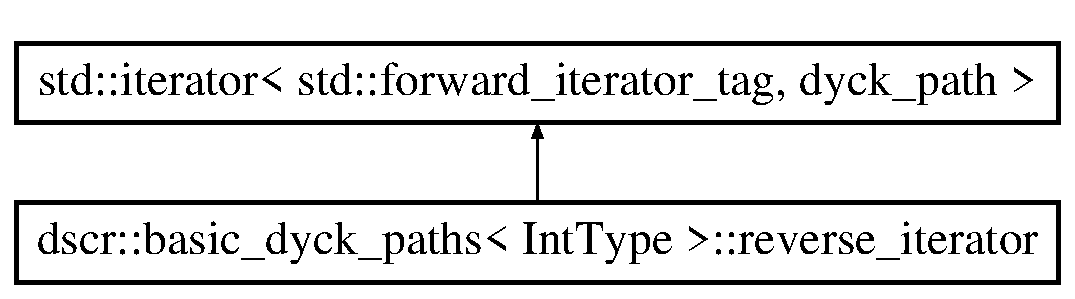
\includegraphics[height=2.000000cm]{classdscr_1_1basic__dyck__paths_1_1reverse__iterator}
\end{center}
\end{figure}
\subsection*{Public Member Functions}
\begin{DoxyCompactItemize}
\item 
\hypertarget{classdscr_1_1basic__dyck__paths_1_1reverse__iterator_a1a8da23270ed1f04a716430ef123ed94}{{\bfseries reverse\-\_\-iterator} (Int\-Type n)}\label{classdscr_1_1basic__dyck__paths_1_1reverse__iterator_a1a8da23270ed1f04a716430ef123ed94}

\item 
\hypertarget{classdscr_1_1basic__dyck__paths_1_1reverse__iterator_a2f04157c9a62a6c909cef492cadca1c8}{\hyperlink{classdscr_1_1basic__dyck__paths_1_1reverse__iterator}{reverse\-\_\-iterator} \& {\bfseries operator++} ()}\label{classdscr_1_1basic__dyck__paths_1_1reverse__iterator_a2f04157c9a62a6c909cef492cadca1c8}

\item 
\hypertarget{classdscr_1_1basic__dyck__paths_1_1reverse__iterator_a7c296ca6c1ff2f5a7204592d34908e6a}{\hyperlink{classdscr_1_1basic__dyck__paths_1_1reverse__iterator}{reverse\-\_\-iterator} \& {\bfseries operator-\/-\/} ()}\label{classdscr_1_1basic__dyck__paths_1_1reverse__iterator_a7c296ca6c1ff2f5a7204592d34908e6a}

\item 
\hypertarget{classdscr_1_1basic__dyck__paths_1_1reverse__iterator_a9fafe50725c4db39251bf14fcc735f50}{const dyck\-\_\-path \& {\bfseries operator$\ast$} ()}\label{classdscr_1_1basic__dyck__paths_1_1reverse__iterator_a9fafe50725c4db39251bf14fcc735f50}

\item 
\hypertarget{classdscr_1_1basic__dyck__paths_1_1reverse__iterator_ad74d38087b1372b933f657f91011924c}{const dyck\-\_\-path \& {\bfseries operator$\ast$} () const }\label{classdscr_1_1basic__dyck__paths_1_1reverse__iterator_ad74d38087b1372b933f657f91011924c}

\item 
\hypertarget{classdscr_1_1basic__dyck__paths_1_1reverse__iterator_a70ea68930164ecb0332c8564fff4295b}{const dyck\-\_\-path $\ast$ {\bfseries operator-\/$>$} () const }\label{classdscr_1_1basic__dyck__paths_1_1reverse__iterator_a70ea68930164ecb0332c8564fff4295b}

\item 
\hypertarget{classdscr_1_1basic__dyck__paths_1_1reverse__iterator_a6b51a1a5018372ef4efe9f73031526a6}{size\-\_\-type {\bfseries I\-D} () const }\label{classdscr_1_1basic__dyck__paths_1_1reverse__iterator_a6b51a1a5018372ef4efe9f73031526a6}

\item 
\hypertarget{classdscr_1_1basic__dyck__paths_1_1reverse__iterator_a6b563b93c9d7cb81c929370eeace8d8b}{bool {\bfseries operator==} (const \hyperlink{classdscr_1_1basic__dyck__paths_1_1reverse__iterator}{reverse\-\_\-iterator} \&it)}\label{classdscr_1_1basic__dyck__paths_1_1reverse__iterator_a6b563b93c9d7cb81c929370eeace8d8b}

\item 
\hypertarget{classdscr_1_1basic__dyck__paths_1_1reverse__iterator_a6527f3e5d4f9afc9d6161c5be5657704}{bool {\bfseries operator!=} (const \hyperlink{classdscr_1_1basic__dyck__paths_1_1reverse__iterator}{reverse\-\_\-iterator} \&it)}\label{classdscr_1_1basic__dyck__paths_1_1reverse__iterator_a6527f3e5d4f9afc9d6161c5be5657704}

\end{DoxyCompactItemize}
\subsection*{Friends}
\begin{DoxyCompactItemize}
\item 
\hypertarget{classdscr_1_1basic__dyck__paths_1_1reverse__iterator_a3dd4f1061ed68889e2068166aee9248a}{class {\bfseries basic\-\_\-dyck\-\_\-paths}}\label{classdscr_1_1basic__dyck__paths_1_1reverse__iterator_a3dd4f1061ed68889e2068166aee9248a}

\item 
\hypertarget{classdscr_1_1basic__dyck__paths_1_1reverse__iterator_a46fe9efd66cb5e2a2e89a93f2e060b82}{difference\-\_\-type {\bfseries operator-\/} (const \hyperlink{classdscr_1_1basic__dyck__paths_1_1reverse__iterator}{reverse\-\_\-iterator} \&lhs, const \hyperlink{classdscr_1_1basic__dyck__paths_1_1reverse__iterator}{reverse\-\_\-iterator} \&rhs)}\label{classdscr_1_1basic__dyck__paths_1_1reverse__iterator_a46fe9efd66cb5e2a2e89a93f2e060b82}

\end{DoxyCompactItemize}


\subsection{Detailed Description}
\subsubsection*{template$<$class Int\-Type$>$class dscr\-::basic\-\_\-dyck\-\_\-paths$<$ Int\-Type $>$\-::reverse\-\_\-iterator}

Reverse random access iterator class. It's much more efficient as a bidirectional iterator than purely random access. 

The documentation for this class was generated from the following file\-:\begin{DoxyCompactItemize}
\item 
Dyck\-Paths.\-hpp\end{DoxyCompactItemize}

\hypertarget{classdscr_1_1_sequence}{\section{dscr\-:\-:Sequence Class Reference}
\label{classdscr_1_1_sequence}\index{dscr\-::\-Sequence@{dscr\-::\-Sequence}}
}


A class to help store known and constant sequences, such as the factorial sequence.  




{\ttfamily \#include $<$Sequences.\-hpp$>$}

\subsection*{Friends}
\begin{DoxyCompactItemize}
\item 
lluint \hyperlink{classdscr_1_1_sequence_a1270a98e6b77cec86abce9542711c0c6}{factorial} (suint n)
\begin{DoxyCompactList}\small\item\em n! \end{DoxyCompactList}\item 
lluint \hyperlink{classdscr_1_1_sequence_a11b1ced236502fd33a7851ae12912387}{binomial} (lluint n, lluint r)
\begin{DoxyCompactList}\small\item\em The number of subsets of size r chosen from a set of size n. \end{DoxyCompactList}\item 
lluint \hyperlink{classdscr_1_1_sequence_ad04fc4341da3f34fa6a57033586a7f76}{catalan} (suint n)
\begin{DoxyCompactList}\small\item\em The n-\/th catalan number. \end{DoxyCompactList}\item 
lluint \hyperlink{classdscr_1_1_sequence_ac733d5b9ab1f17f2e37cbcecffb985c0}{motzkin} (suint n)
\begin{DoxyCompactList}\small\item\em The n-\/th motzkin number. \end{DoxyCompactList}\item 
\hypertarget{classdscr_1_1_sequence_a7e719c2c0234b0c82e1bbd0dc0a7ca61}{lluint {\bfseries partition\-\_\-number} (suint n)}\label{classdscr_1_1_sequence_a7e719c2c0234b0c82e1bbd0dc0a7ca61}

\end{DoxyCompactItemize}


\subsection{Detailed Description}
A class to help store known and constant sequences, such as the factorial sequence. 

\subsection{Friends And Related Function Documentation}
\hypertarget{classdscr_1_1_sequence_a11b1ced236502fd33a7851ae12912387}{\index{dscr\-::\-Sequence@{dscr\-::\-Sequence}!binomial@{binomial}}
\index{binomial@{binomial}!dscr::Sequence@{dscr\-::\-Sequence}}
\subsubsection[{binomial}]{\setlength{\rightskip}{0pt plus 5cm}lluint binomial (
\begin{DoxyParamCaption}
\item[{lluint}]{n, }
\item[{lluint}]{r}
\end{DoxyParamCaption}
)\hspace{0.3cm}{\ttfamily [friend]}}}\label{classdscr_1_1_sequence_a11b1ced236502fd33a7851ae12912387}


The number of subsets of size r chosen from a set of size n. 


\begin{DoxyParams}{Parameters}
{\em n} & is a (small) nonnegative integer \\
\hline
{\em r} & is a small integer between 0 and n (inclusive) \\
\hline
\end{DoxyParams}
\begin{DoxyReturn}{Returns}
n!/(r!$\ast$(n-\/r)!) 
\end{DoxyReturn}
\hypertarget{classdscr_1_1_sequence_ad04fc4341da3f34fa6a57033586a7f76}{\index{dscr\-::\-Sequence@{dscr\-::\-Sequence}!catalan@{catalan}}
\index{catalan@{catalan}!dscr::Sequence@{dscr\-::\-Sequence}}
\subsubsection[{catalan}]{\setlength{\rightskip}{0pt plus 5cm}lluint catalan (
\begin{DoxyParamCaption}
\item[{suint}]{n}
\end{DoxyParamCaption}
)\hspace{0.3cm}{\ttfamily [friend]}}}\label{classdscr_1_1_sequence_ad04fc4341da3f34fa6a57033586a7f76}


The n-\/th catalan number. 


\begin{DoxyParams}{Parameters}
{\em n} & is a (small) nonnegative integer \\
\hline
\end{DoxyParams}
\begin{DoxyReturn}{Returns}
binomial(2n,n)/(n+1) 
\end{DoxyReturn}
\hypertarget{classdscr_1_1_sequence_a1270a98e6b77cec86abce9542711c0c6}{\index{dscr\-::\-Sequence@{dscr\-::\-Sequence}!factorial@{factorial}}
\index{factorial@{factorial}!dscr::Sequence@{dscr\-::\-Sequence}}
\subsubsection[{factorial}]{\setlength{\rightskip}{0pt plus 5cm}lluint factorial (
\begin{DoxyParamCaption}
\item[{suint}]{n}
\end{DoxyParamCaption}
)\hspace{0.3cm}{\ttfamily [friend]}}}\label{classdscr_1_1_sequence_a1270a98e6b77cec86abce9542711c0c6}


n! 


\begin{DoxyParams}{Parameters}
{\em n} & is a (small) nonnegative integer. \\
\hline
\end{DoxyParams}
\begin{DoxyReturn}{Returns}
n! 
\end{DoxyReturn}
\hypertarget{classdscr_1_1_sequence_ac733d5b9ab1f17f2e37cbcecffb985c0}{\index{dscr\-::\-Sequence@{dscr\-::\-Sequence}!motzkin@{motzkin}}
\index{motzkin@{motzkin}!dscr::Sequence@{dscr\-::\-Sequence}}
\subsubsection[{motzkin}]{\setlength{\rightskip}{0pt plus 5cm}lluint motzkin (
\begin{DoxyParamCaption}
\item[{suint}]{n}
\end{DoxyParamCaption}
)\hspace{0.3cm}{\ttfamily [friend]}}}\label{classdscr_1_1_sequence_ac733d5b9ab1f17f2e37cbcecffb985c0}


The n-\/th motzkin number. 


\begin{DoxyParams}{Parameters}
{\em n} & is a (small) nonnegative integer \\
\hline
\end{DoxyParams}
\begin{DoxyReturn}{Returns}
M\-\_\-n 
\end{DoxyReturn}


The documentation for this class was generated from the following files\-:\begin{DoxyCompactItemize}
\item 
Sequences.\-hpp\item 
Sequences.\-cpp\end{DoxyCompactItemize}

%--- End generated contents ---

% Index
\newpage
\phantomsection
\addcontentsline{toc}{part}{Index}
\printindex

\end{document}
